
%----------------------------------------------------------------------------------------
%	PACKAGES AND DOCUMENT CONFIGURATIONS
%----------------------------------------------------------------------------------------

\documentclass{scrartcl}

\usepackage{siunitx} % Provides the \SI{}{} command for typesetting SI units
\usepackage{booktabs}

\usepackage{hyperref}
\usepackage{xspace}
\usepackage{color}
\usepackage{array}

\usepackage{graphicx} % Required for the inclusion of images
\usepackage{listings}
\usepackage[toc, nonumberlist]{glossaries} % must go after hyperref, so entries are clickable
%\setlength\parindent{0pt} % Removes all indentation from paragraphs

%\renewcommand{\labelenumi}{\alph{enumi}.} % Make numbering in the enumerate environment by letter rather than number (e.g. section 6)

%----------------------------------------------------------------------------------------
%	DOCUMENT INFORMATION
%----------------------------------------------------------------------------------------

\def\etal {{\it et~al.}}

\def\pxar {{pXar}\xspace}

\def\cmake {{\tt cmake}\xspace}

\newcommand{\fixme[1]} {\textcolor{red}{FIXME: #1}\xspace}

\newcolumntype{L}{>{\centering\arraybackslash}m{5.7cm}}

\def\iana {\textcolor{blue}{$\textrm{I}_{\textrm{ana}}$}\xspace}
\def\vcal {\textcolor{blue}{$\textrm{V}_{\textrm{cal}}$}\xspace}
\def\vana {\textcolor{blue}{$\textrm{V}_{\textrm{ana}}$}\xspace}
\def\caldel {\textcolor{blue}{CalDel}\xspace}
\def\vthrcomp {\textcolor{blue}{$\textrm{V}_{\textrm{thr}}$Comp}\xspace}
\def\vtrim {\textcolor{blue}{$\textrm{V}_{\textrm{trim}}$}\xspace}
\def\trimbits {\textcolor{blue}{Trim bits}\xspace}
\def\phoffset {\textcolor{blue}{PHOffset}\xspace}
\def\phscale {\textcolor{blue}{PHScale}\xspace}

%\def\testparameters {{\tt testparameters.dat}\xspace}
%\def\usertests {{\tt pxar/usertests}\xspace}
\def\fulltest {{\tt FullTest}\xspace}
\def\pretest {{\tt PreTest}\xspace}
\def\alivetest {{\tt PixelAlive}\xspace}
\def\trimming {{\tt Trimming}\xspace}
\def\trim {{\tt Trim}\xspace}
\def\trimbit {{\tt TrimBits}\xspace}
\def\phopt {{\tt PHOptimization}\xspace}
\def\gainped {{\tt GainPedestal}\xspace}
\def\scurves {{\tt SCurve}\xspace}
\def\bb {{\tt BumpBonding}\xspace}
\def\iv {{\tt IV}\xspace}

\def\dac {{\tt DAC}\xspace}
\def\dacs {{\tt DAC}s\xspace}

\def\roc {{ROC}\xspace}
\def\rocs {{ROCs}\xspace}
\def\ph {{pulse height}\xspace}





% Load glossary
%\loadglsentries{usermanual/glossary.tex}

\renewcommand*\glsgroupskip{}
\renewcommand*{\glspostdescription}{.\vspace{-0.5\baselineskip}}
%\makeglossaries

\title{FPix Module Testing Reference Guide} % Title

\author{
J. Antonelli, 
P. Merkel
} % Author names

\date{\today} % Date for the report

\begin{document}

\maketitle % Insert the title, author and date


\begin{abstract}
The document provides an overview of the module testing methodology and procedures used for the CMS Forward Pixel Phase I Upgrade project. 
It briefly introduces the individual components of a pixel module and describes the module assembly procedures.
It then describes in greater detail all the individual tests performed during module testing and calibration, discussed in the other that the tests are normally performed. 
Finally, it describes the standard procedure for testing modules at Fermilab and saving the test results for visualization and grading purposes.
\\\\\\\\
TO DO LIST 9-10-2015:
\\
Note: \textcolor{red}{RED text implies the section is incomplete.}
\begin{enumerate}
\item finish methodology section for each test
\item write testing procedure section
\item update to latest pxar release and run full test to get example output
\item write output section for each test
\item write database uploading section - need input from Doug/John
\item write grading scheme section - need input from Petra/Doug/John
\item integrate testing sections into pxar git repo
\end{enumerate}

\end{abstract}

\newpage
% Table Of Contents
\tableofcontents

\newpage
% ======================================================================
\section{FPix Module Components}
\label{s:components}
% ======================================================================

The pixel module for the CMS Phase I upgrade consists of several discrete components, manufactured by independent contractors.  
The silicon sensor is the active unit of the module, converting energy deposited by incident particles into an electrical signal.  
Each sensor contains 66,560 individual pixels.  
The standard pixel size is 100 $\mu$m $\times$ 150 $\mu$m, although some edge pixels are twice as large in the dimension perpendicular to the sensor edge.  

The psi46 readout chip (ROC) is an ~8 mm square integrated circuit that takes the signal from the sensor, 
processes it, and packages the data to be sent onward in the readout chain.  
Each ROC covers an array of 80 $\times$ 52 pixels (4160 pixels).  

The high density interconnect (HDI) is a printed flexible circuit that accepts the data from multiple ROCs 
and combines it to be transmitted to the central CMS data acquisition (DAQ) system.  
The serialization of the data is performed by the token bit manager (TBM) which is a logic chip glued onto the HDI.

%\newpage
% ======================================================================
\section{FPix Module Construction}
\label{s:contruction}
% ======================================================================

Module assembly takes place in several independent steps at multiple locations.  
First, the sensor is attached to 16 ROCs by the company RTI using a bump-bonding technique.  
Balls of lead/tin solder, roughly 30-40 $\mu$m in diameter, are deposited onto the ROCs.  
Then each ROC is aligned to the sensor and the two are pressed together to complete the electrical connection.

HDIs, produced by Compunetics, are delivered to Fermilab where all the surface components (including the TBM) are mounted.

The combination of 16 ROCs bump-bonded to a sensor is referred to as a “bare module”.  
RTI sends the bare modules to the two FPix assembly site at Purdue University and The University of Nebraska.  
At the assembly sites, the completed HDIs are glued to the top of the sensor side of the bare modules.  
Then the readout pads of the ROCs are connected to the input pads of the HDI via thin wires in a process referred to as wirebonding.  
The complete modules are tested for basic functionality, and any correctable errors (e.g. broken wirebonds) are addressed.

The modules are then shipped to one of three FPix testing sites:  
Fermilab (FNAL), University of Kansas (KU), and University of Illinois-Chicago (UIC).  
KU and UIC are equipped with X-ray testing setups, 
while FNAL is the central testing site where the final calibration and grading is performed.  
This document will detail the testing procedures at FNAL, as X-ray testing is covered in a separate document.

%\newpage
% ======================================================================
\section{The Pixel Unit Cell}
\label{s:puc}
% ======================================================================

The bulk of module testing concerns the pixel unit cell (PUC) of the \roc.  
For this reason, it is useful to discuss the design and operation of the PUC.  
Figure~\ref{fig:puc} shows the elements of the PUC, the double column periphery, and the controller and interface block.  
It is labeled with some of the \dac registers that are most relevant for module testing.  
Terms in black boxes represent programmable \dac registers on the \roc.
While all \dac memory registers are \roc-wide and exist at the periphery (except the 4 \trimbits), 
the diagram shows \dacs next to the circuit element they directly affect.
For the remainder of this document, these \dac registers will be denoted with \textcolor{blue}{blue text}.  
The process of calibrating a module is largely comprised of tests that find and set the optimal values for these parameters.  

\begin{figure*}[hbtp]
\begin{center}
\includegraphics[width=\textwidth]{figures/ROC_dac_schematic.pdf}
\caption{A schematic of the circuit components and the relevant programmable registers within the \roc.}
\label{fig:puc}
\end{center}
\end{figure*}

The signal processing within the PUC begins with an amplifier and shaper that convert the incident current into a reformatted voltage signal.  
The signal is then fed into a voltage comparator, 
the threshold of which is controlled by \vthrcomp with additional inputs possible from \vtrim and the \trimbits.  
If the input signal exceeds the comparator's threshold, 
the signal is stored for readout and the pixel notifies the logic at the periphery of the double column 
that a hit has been registered and is ready to be transferred to the data buffer at the periphery.   
This initiates the double column drain mechanism, 
transferring pulse height (PH) values from any pixel with a hit registered since the previous drain onto the 80-wide PH buffer on the periphery.
In addition to the ability to process charge produced by particles passing through the silicon sensor, 
the \roc can produce an internal calibration signal whose amplitude is controlled via the \vcal~\dac.  
This calibration signal serves as the input to the PUC in almost all of the tests described in this document.
Table~\ref{tab:daclist} shows a subset of \dac registers in the PUC and explains their usage.
\\\\

\begin{table}[htbp]
\caption{List of \dac registers relevant to module testing.  \dac names are denoted with \textcolor{blue}{blue} text.}
\renewcommand{\arraystretch}{1.2}\begin{tabular}{|c|L|L|}
\hline
\dac Name & Usage & Tests that optimize this \dac \\
\hline
\hline
\vcal & Calibration signal voltage. There are two \vcal ranges (low and high) with the high range being roughly 7 times larger.  
The choice of low/high range is set via the \textcolor{blue}{CtrlReg} \dac. & None - set to an appropriate level depending on the test\\
\hline
\vana & Voltage supplied to the analog part of the PUC (amplifier and shaper) & \pretest ({\tt SetVana}) \\
\hline
\caldel & Delay in sending out calibration pulse with respect to the clock signal & \pretest ({\tt SetVthrCompCalDel}) \\
\hline
\vthrcomp & Voltage supplied to the comparator unit, inversely related to the signal voltage required to fire the comparator (i.e. the comparator threshold) & \pretest ({\tt SetVthrCompCalDel}), \trimming \\
\hline
\vtrim & Additional voltage supplied to the comparator unit to decrease the threshold (in conjunction with the \trimbits) & \trimming \\
\hline
\trimbits & 4 bits per PUC that decrease the threshold of the comparator unit & \trimming \\
\hline
\phoffset & Constant offset added to the pulse height & \phopt \\
\hline
\phscale & Sets the slope of the PH vs. input signal strength curve & \phopt \\
\hline
\end{tabular}
\label{tab:daclist}
\end{table}

%\newpage
% ======================================================================
\section{Modules Tests}
\label{s:tests}
% ======================================================================

Modules are tested using the pXar software framework.  
More information on pXar can be found at https://twiki.cern.ch/twiki/bin/viewauth/CMS/Pxar.

% ----------------------------------------------------------------------

% ----------------------------------------------------------------------
\subsection{\pretest}
\label{ss:pretest}

\subsubsection{Purpose}

The \pretest is meant to put the module into an operational state in preparation for more specific tests.
The basic operation of the \roc is checked and some of the default \dac settings are tested.

\subsubsection{Methodology}

In the {\tt ProgramRoc} subtest, the ``programmability'' of the \roc is tested.
The value of the current drawn by the analog amplifiers in all the PUCs (\iana) is measured.
This is done first with the nominal value of \vana, and then again with \vana set to zero.
The difference in \iana from these two measurements should be non-zero,
signifying that \vana is actually being applied to the \roc.
This implies the \roc is capable of receiving commands to alter \dac values, i.e. it is programmable.
Its output is shown in Figure~\ref{fig:pretest_programROC}.
\\\\
The {\tt SetVana} subtest sets the \vana~\dac so that the total current draw (\iana) meets a target value (default is 24 mA).
\vana is iteratively adjusted from its default value until it comes within 0.25 mA of the target 
or until 10 iterations have been performed.  The output is shown in Figures~\ref{fig:pretest_Iana} and~\ref{fig:pretest_VanaSettings}.
%\\\\
% Note: as of 9-11-15, the timing test isn't run as part of the fulltest
%The {\tt SetTimings} test \textcolor{red}{FIXME – talk to Doug}
\\\\
The {\tt SetVthrCompCalDel} subtest optimizes the values of the \vthrcomp and \caldel~\dacs.
A sample pixel is chosen from within each \roc for this test and is assumed to be representative of normal pixel performance.
A scan is performed over \vthrcomp and \caldel to determine which combinations of them put the pixel into an operational state.
At each point in the 256 $\times$ 256 value parameter space,
a number of calibration pulses (default is 5) are sent to the PUC of the sample pixel.
The number of hits successfully recorded by the pixel is then calculated,
and the results are displayed in the 2D plane of \vthrcomp vs. \caldel values
in what is referred to as a ``tornado plot'' (they looked more like tornados with the older, analog \roc).
Figure~\ref{fig:pretest_pretestVthrCompCalDel_c12_r22} shows a tornado plot.
The red region corresponds to 100\% efficiency \textendash\xspace 
the operational region for the PUC with respect to \vthrcomp and \caldel.
Recall that \vthrcomp is inversely related to the minimum pulse height required to fire the comparator.
The region of \vthrcomp $>$ 150 has zero efficiency because
the threshold of the comparator is so low that the pixel is constantly firing on electronic noise,
and when the calibration pulse is injected,
the pixel is already in an unresponsive state waiting to be read out.
By default \vthrcomp is set 50 units higher than the lower edge of the operating plateau,
and \caldel is set halfway between the left and right edges of the plateau at the chosen \vthrcomp value.
The black dot centered within the white square denotes the chosen working point for these two parameters.
Figure~\ref{fig:pretest_pretestCalDel} shows the values of \caldel chosen by the test.

\subsubsection{Output}

\begin{figure}[!htp]
\centering
\begin{minipage}{0.45\textwidth}
  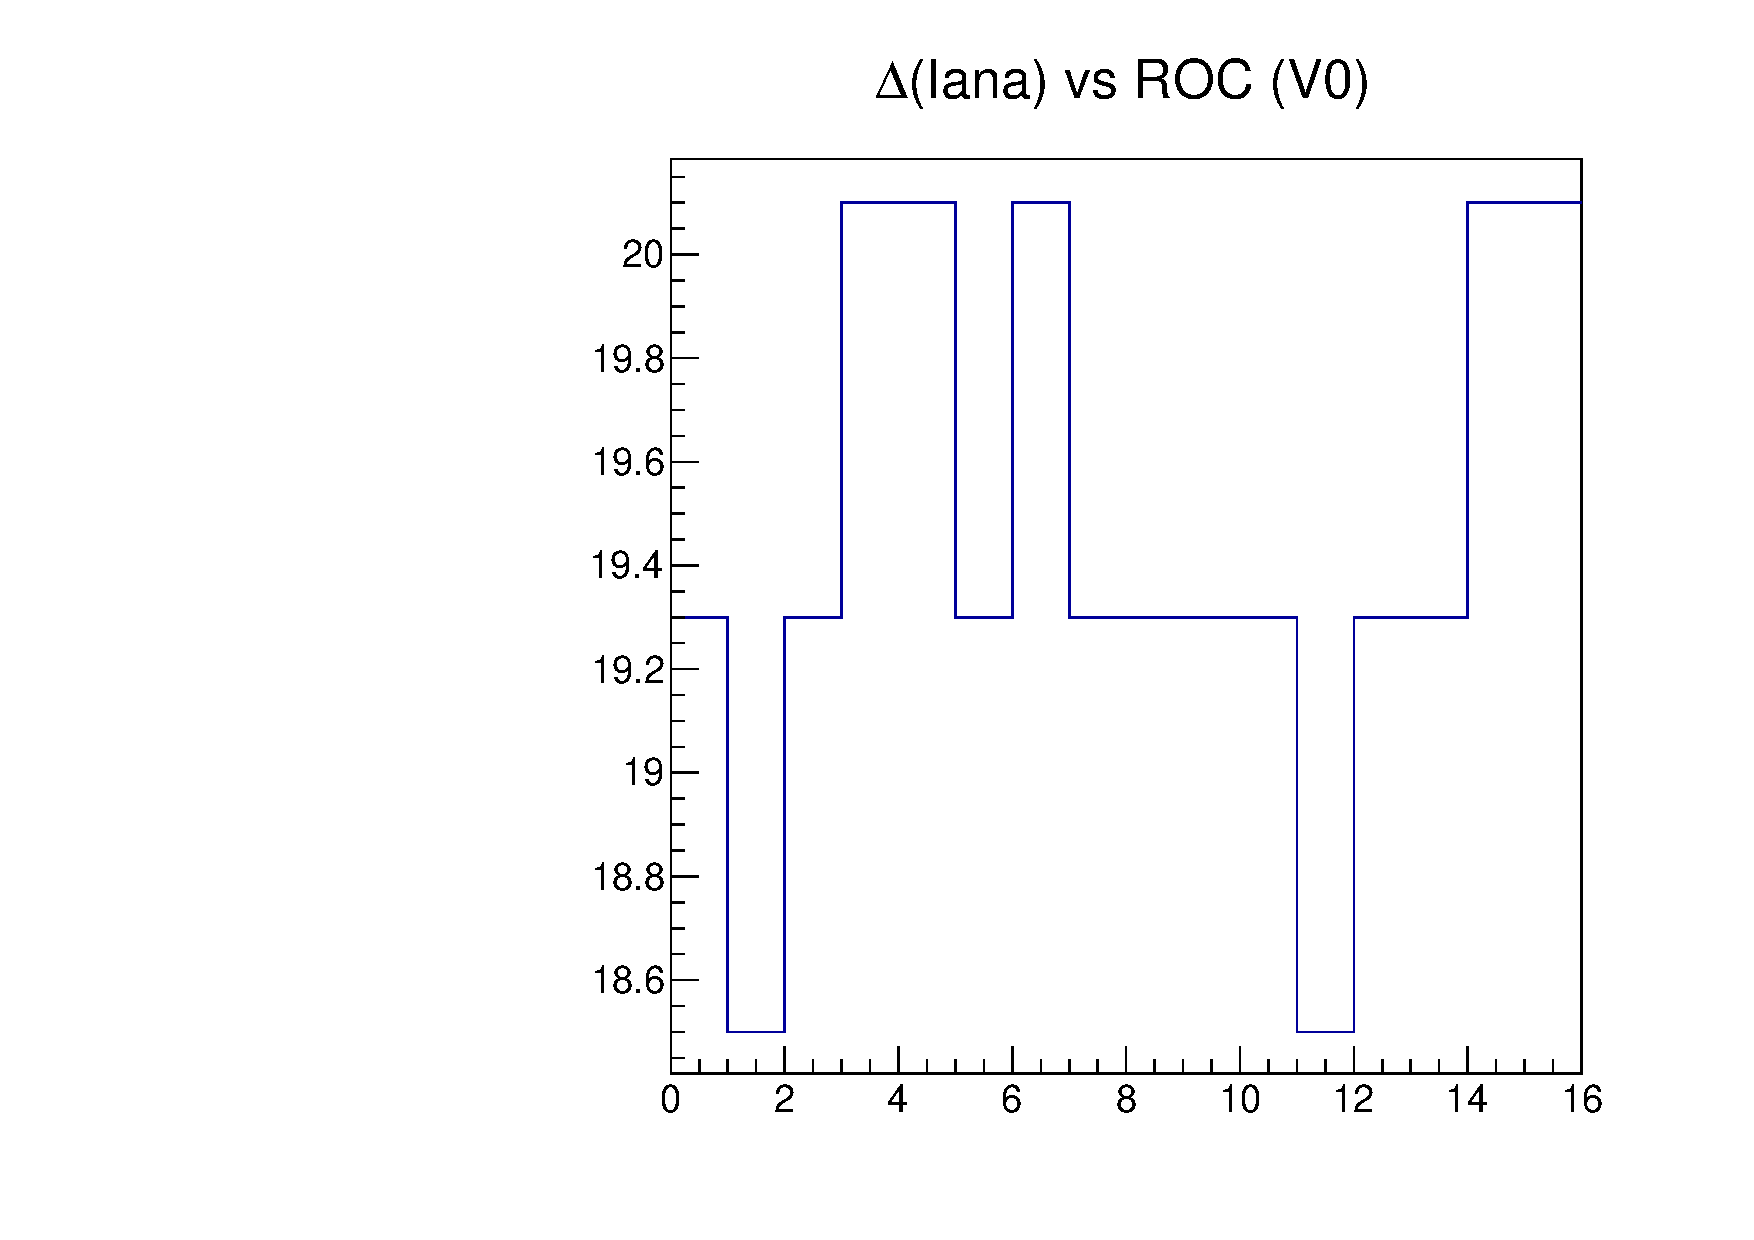
\includegraphics[width=1.0\textwidth]{figures/pretest_programROC.pdf}
  \caption{Created by the {\tt ProgramRoc} subtest. 
    Plotted is the difference in \iana for cases of \vana on/off, as a function of \roc number.
    Values for programmable \rocs are non-zero.}
  \label{fig:pretest_programROC}
\end{minipage}
\hspace{0.3cm}
\begin{minipage}{0.45\textwidth}
  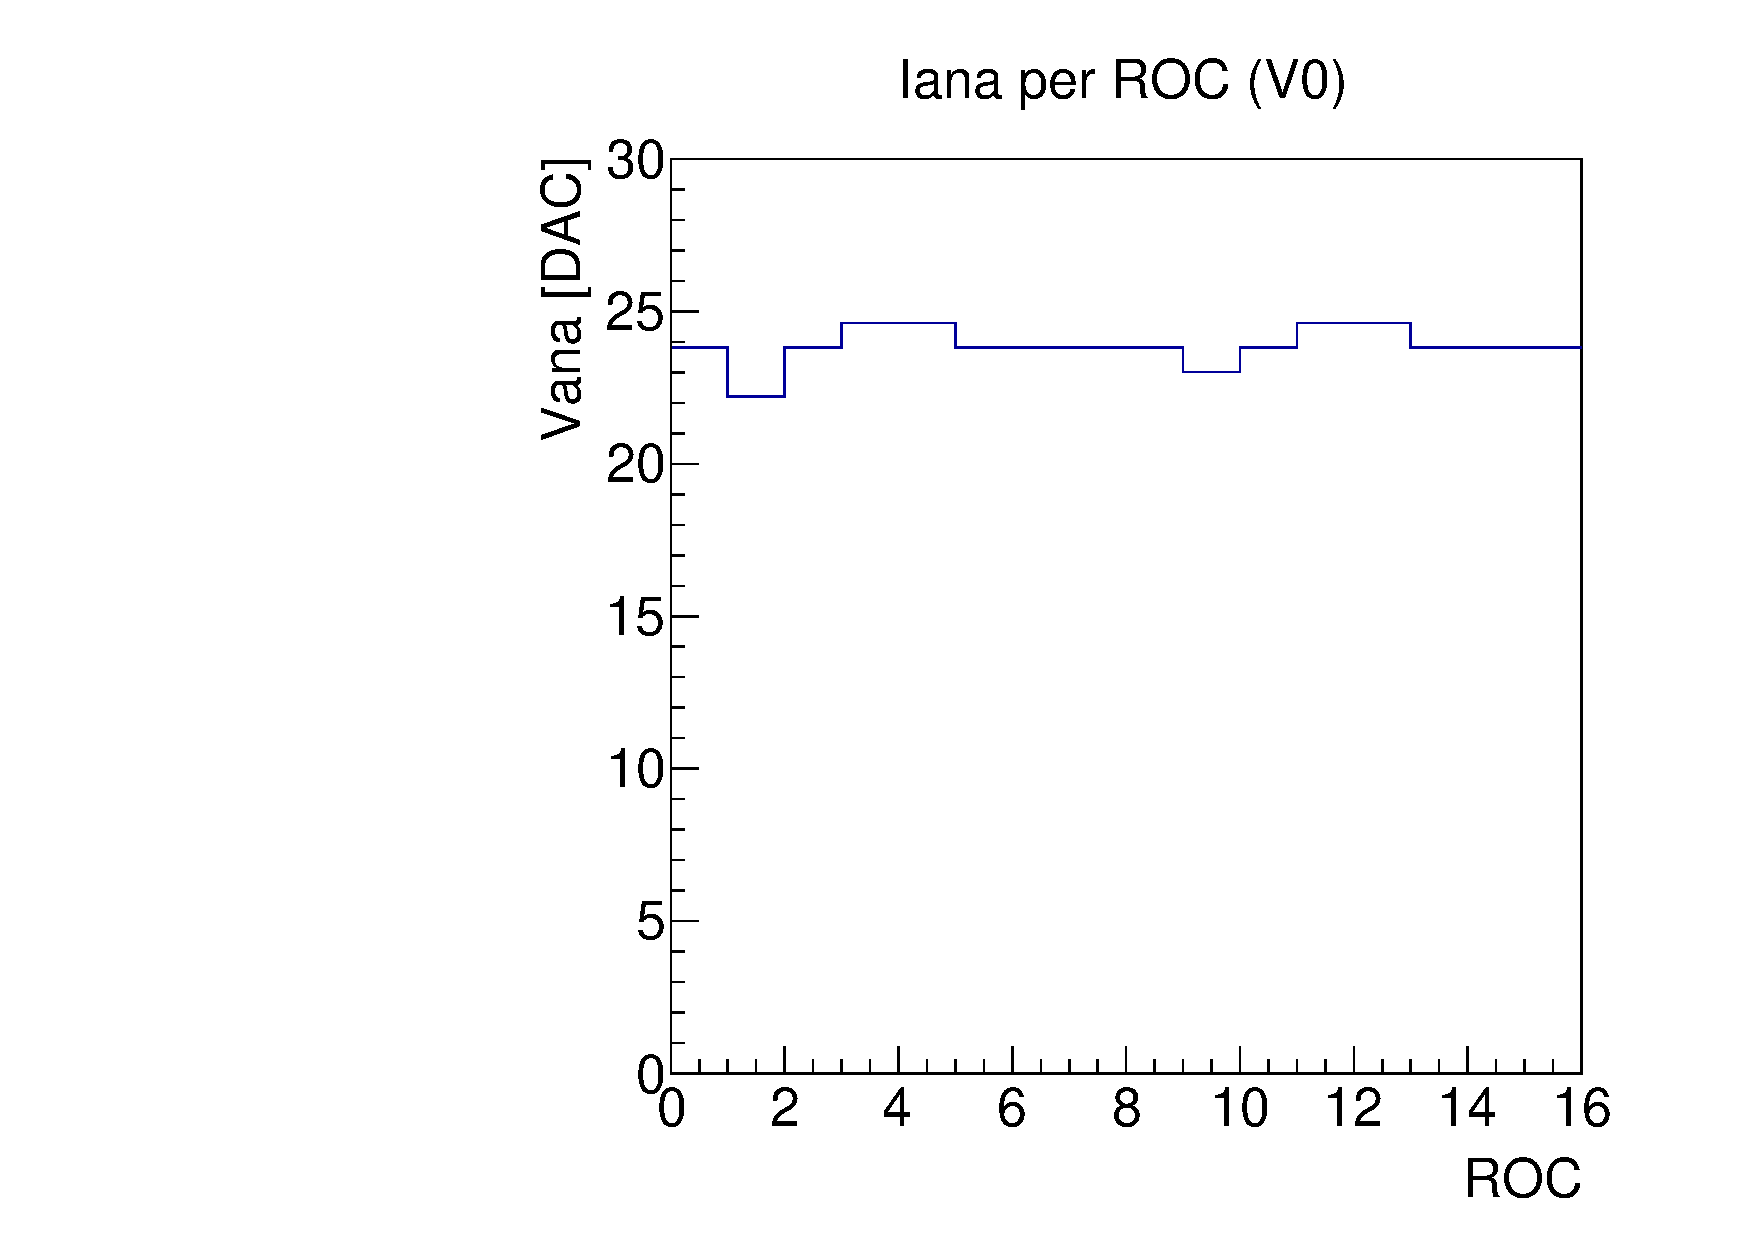
\includegraphics[width=1.0\textwidth]{figures/pretest_Iana.pdf}
  \caption{Created by the {\tt SetVana} subtest.  
    Plotted are the final values of \iana (typo in y-axis label), as a function of \roc number.
    The default target value for \iana is 24 mA.}
  \label{fig:pretest_Iana}
\end{minipage}
\end{figure}

\begin{figure}[!htp]
\centering
\begin{minipage}{0.45\textwidth}
  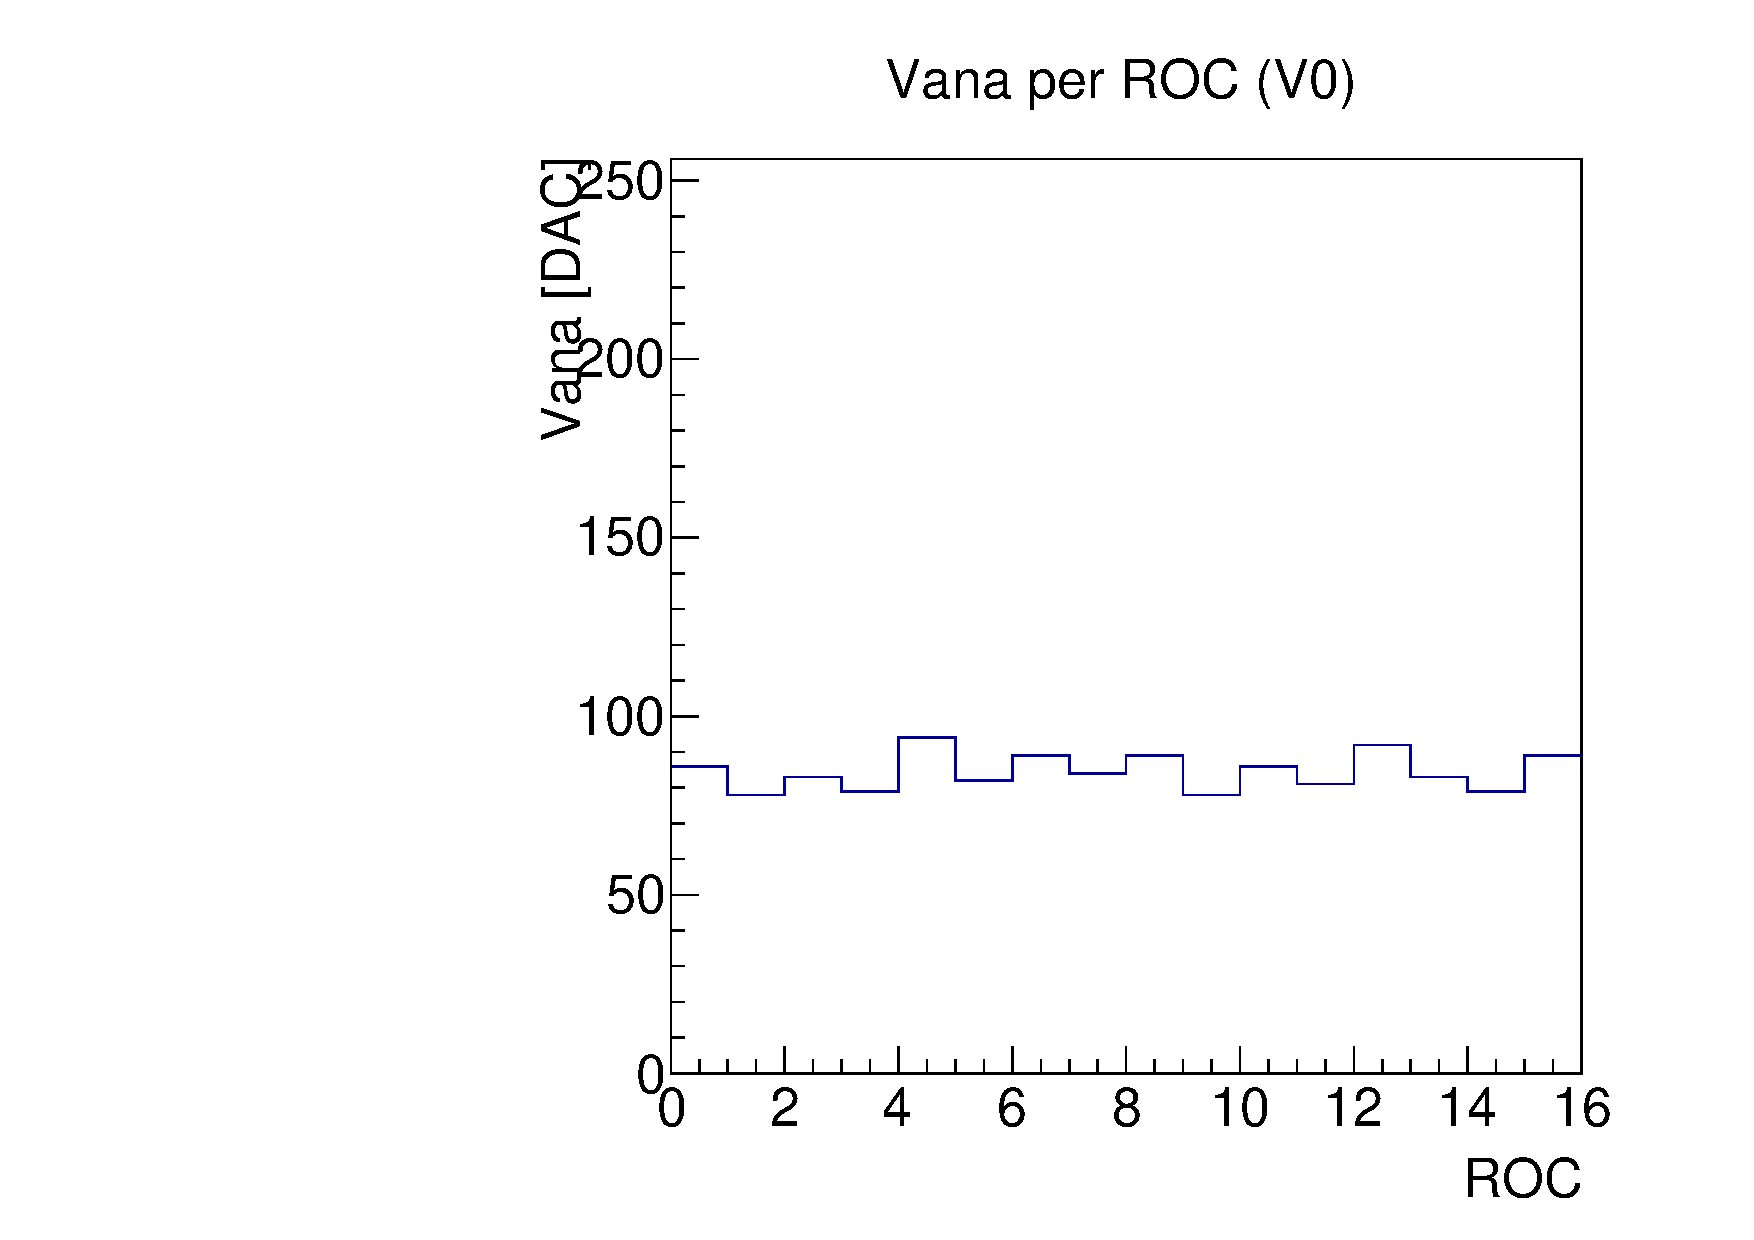
\includegraphics[width=1.0\textwidth]{figures/pretest_VanaSettings.pdf}
  \caption{Created by the {\tt SetVana} subtest.  
    Plotted are the optimized values of \vana, as a function of \roc number.
    For the default \iana target of 24 mA, \vana is roughly 80 DAC units.}
  \label{fig:pretest_VanaSettings}
\end{minipage}
\hspace{0.3cm}
\begin{minipage}{0.45\textwidth}
  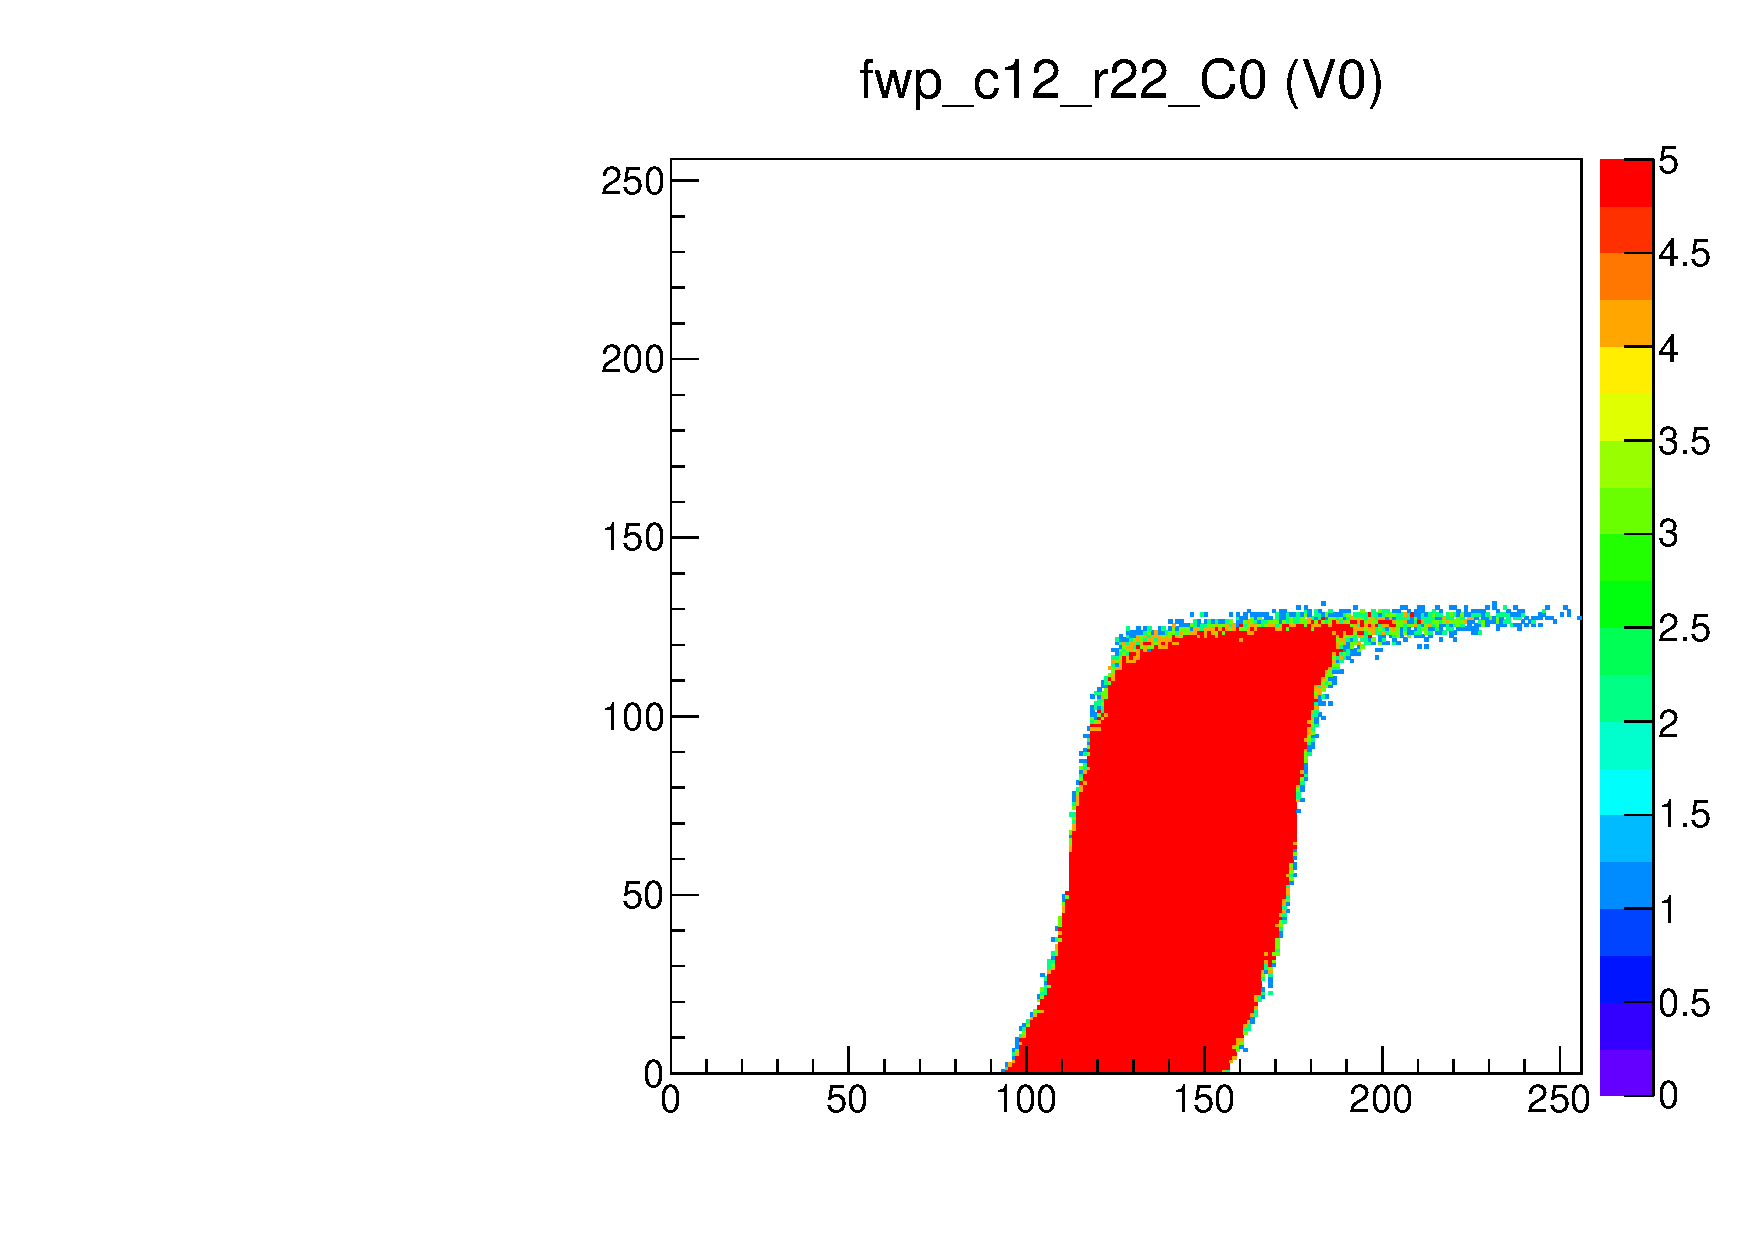
\includegraphics[width=1.0\textwidth]{figures/pretest_fwp_c12_r22.pdf}
  \caption{Created by the {\tt FindWorkingPixel} subtest.
  Similar to Figure~\ref{fig:pretest_pretestVthrCompCalDel_c12_r22}.}
  \label{fig:pretest_fwp_c12_r22}
\end{minipage}
\end{figure}

\begin{figure}[!htp]
\centering
\begin{minipage}{0.45\textwidth}
  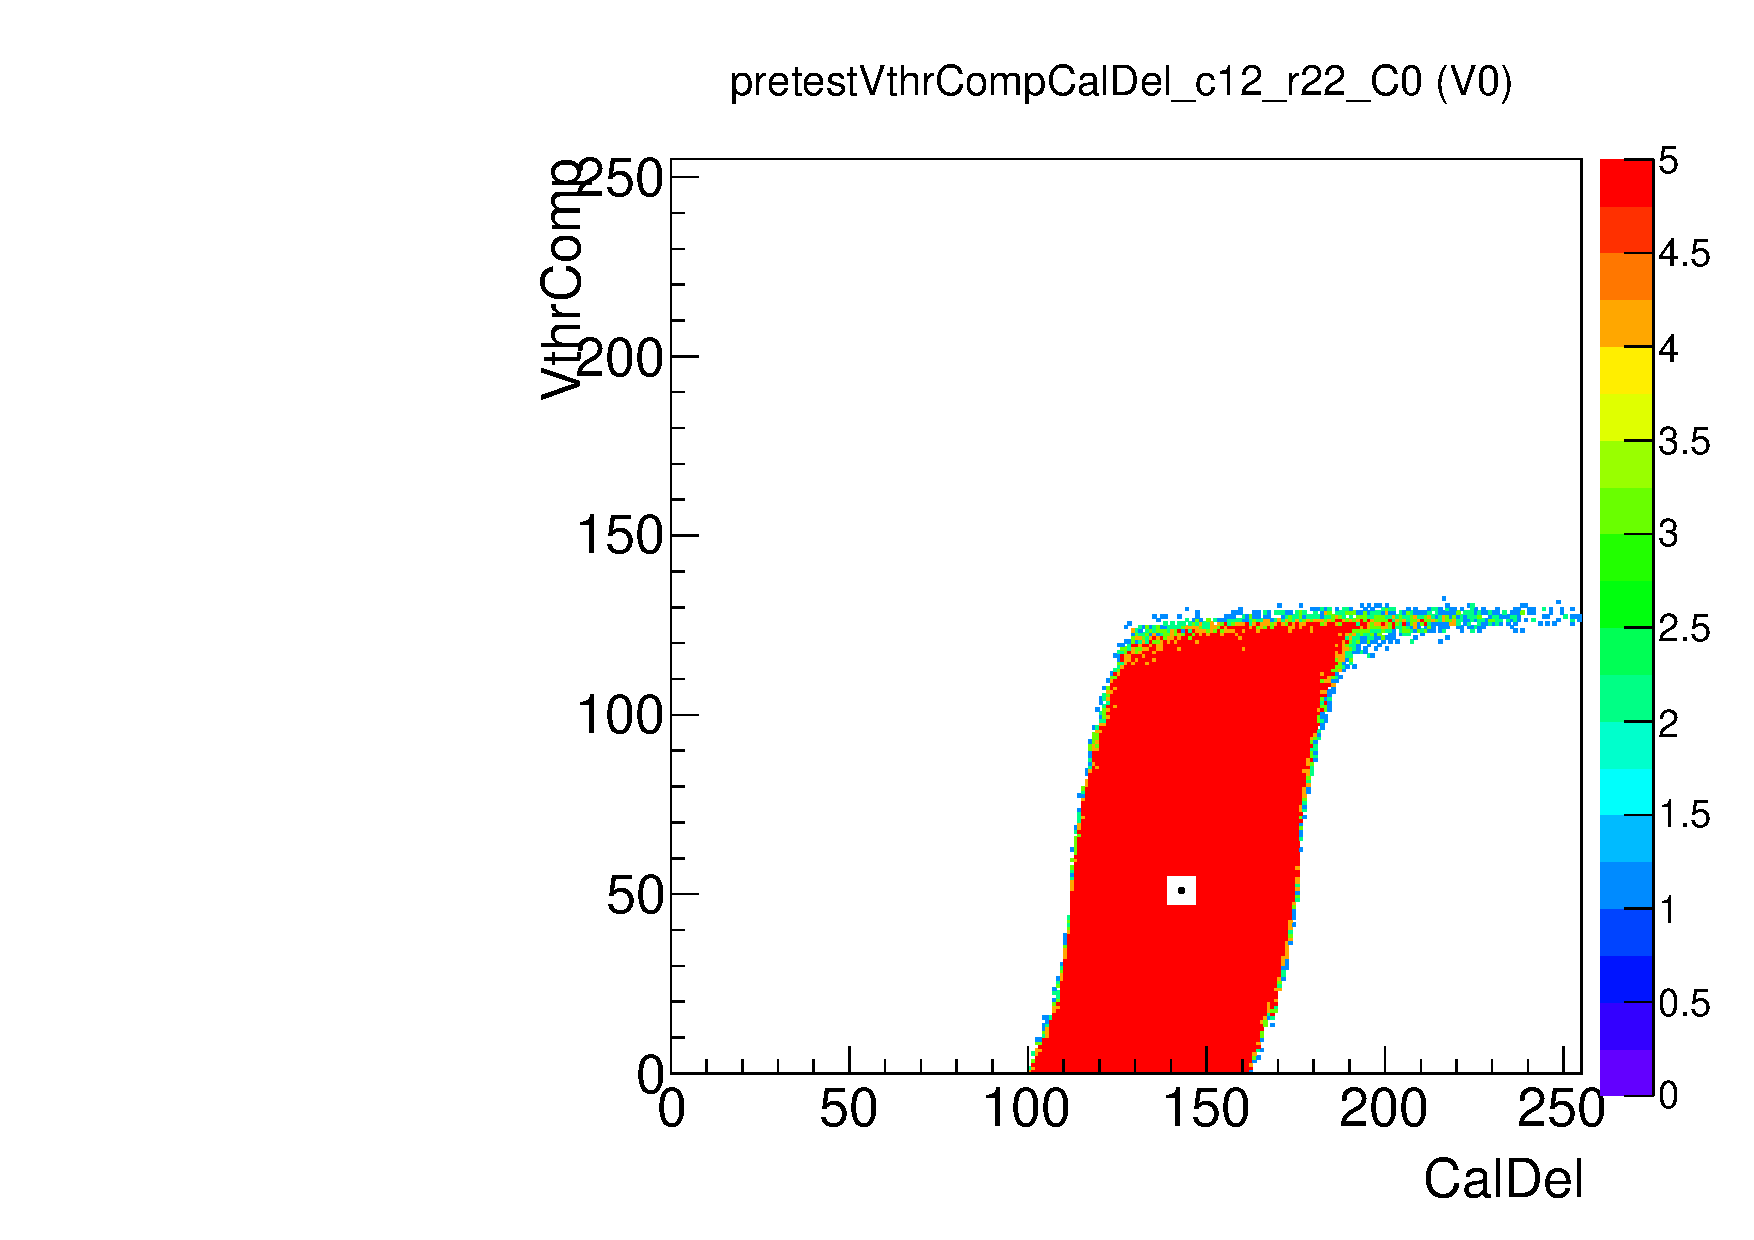
\includegraphics[width=1.0\textwidth]{figures/pretest_pretestVthrCompCalDel_c12_r22.pdf}
  \caption{Tornado plot (efficiency in the \vthrcomp vs. \caldel plane).}
  \label{fig:pretest_pretestVthrCompCalDel_c12_r22}
\end{minipage}
\hspace{0.3cm}
\begin{minipage}{0.45\textwidth}
  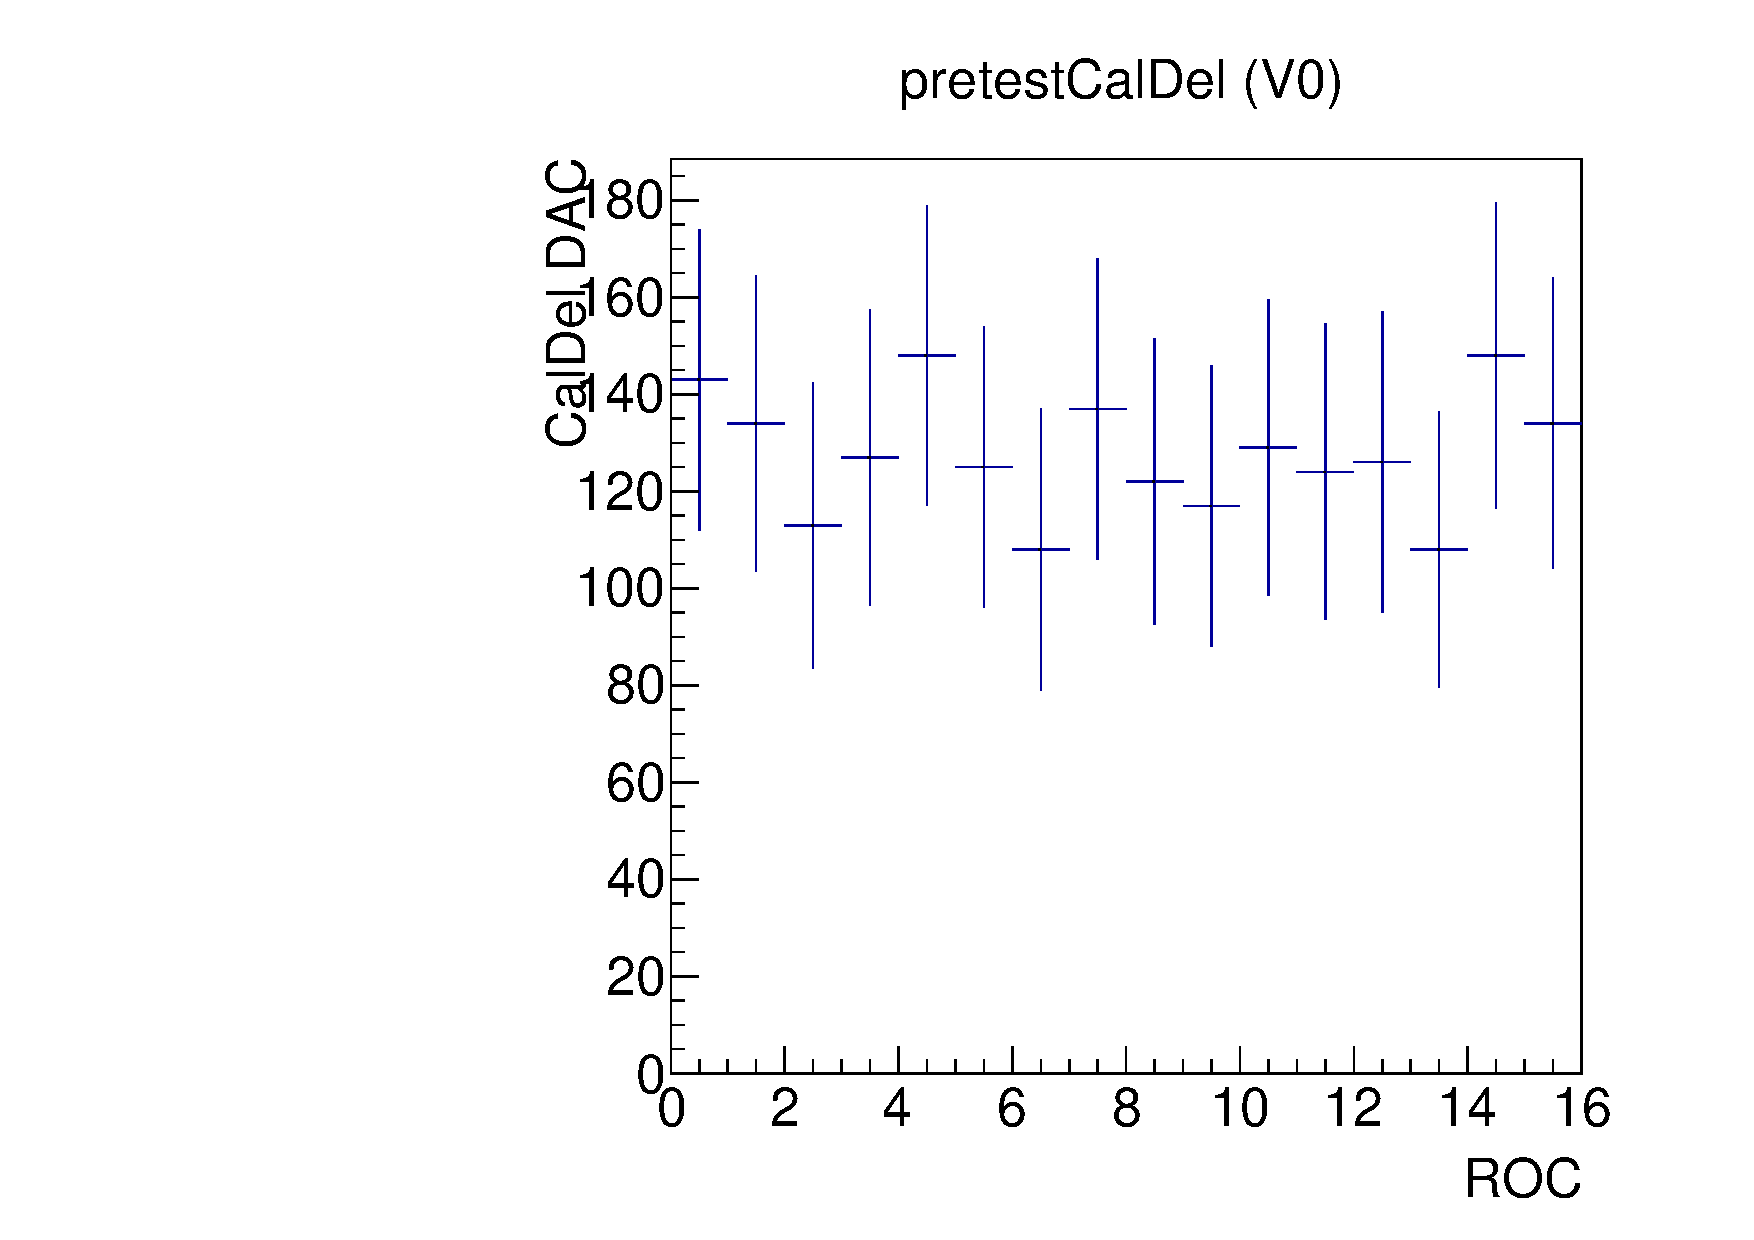
\includegraphics[width=1.0\textwidth]{figures/pretest_pretestCalDel.pdf}
  \caption{The chosen values of \caldel as a function of \roc number.}
  \label{fig:pretest_pretestCalDel}
\end{minipage}
\end{figure}




% ----------------------------------------------------------------------

\newpage

\subsection{\alivetest Test}
\label{ss:alive}

\subsubsection{Purpose}

Once the pretest is completed, we can be relatively sure that all non-faulty pixels should respond to the calibration pulse.
The \alivetest test uses this fact to identify faulty pixels.
Because a pixel can be faulty in multiple ways, this test flags three types of defective pixels:
dead pixels, unmaskable pixels, and pixels with addressing errors.

\subsubsection{Methodology}

In the {\tt Alive} test, a number of calibration pulses (default 10) are sent, in turn,
to each pixel in the device and the number of signals recorded is measured.
During this period, all pixels other than the one being tested are masked, so as not to produce spurious noise signals.
Pixels with no recorded hits are flagged as dead and pixels with less than 100\% efficiency are flagged as problematic.
\\\\
In the {\tt Mask} test, all pixels are disabled and the same procedure is performed.
Pixels with efficiency above zero have a problem with the pixel masking procedure, and are flagged as bad.
\\\\
In the {\tt AddressDecoding} test, the same efficiency measurement is performed, pixel by pixel,
but the order of the resulting data is checked.
If the address of a given pixel is out of order, the recorded hit is given a negative pulse height value.
Pixels with negative hits are flagged as faulty.

\subsubsection{\textcolor{red}{Output}}


% ----------------------------------------------------------------------

\newpage

\subsection{\trimming Test}
\label{ss:trimming}

\subsubsection{Purpose}

The \trimming test accounts for variations in the sensitivities of the 4,160 PUCs within a \roc.
By using the combined effect of the \vthrcomp, \vtrim, and \trimbits,
it attempts to calibrate every PUC to the same threshold with respect to the calibration pulse strength.
These \dacs can be seen in Figure~\ref{fig:puc} as inputs into the ``trimming'' and ``comparator'' elements of the PUC.
\vtrim sets a course scale for the trimming and the \trimbits further fine tune the trimming.
While \vthrcomp and \vtrim are \roc-wide values, there exist four \trimbits for every pixel in a \roc.
``Trimming'' a \roc using \vtrim and the \trimbits effectively means reducing the signal amplitude required to fire the comparator.
Once a module is ``trimmed'', all pixels should turn on at a user-defined threshold (default is \vcal = 35 (low range)).
Thus, input signals with less strength than this threshold will not fire the comparator and will not be registered as a hit.
This ensures that all pixels within a module have a uniform level of zero-suppression.
Additionally, the \trimbit subtest verifies that all trim bits are working
by sequentially flipping each bit off and on and observing its effect.

\subsubsection{Methodology}

It's important to understanding the relevant \dacs for this test: \vthrcomp, \vtrim, and the \trimbits.
\vthrcomp sets a baseline threshold for the comparator unit.
This threshold can be reduced (i.e. ``trimmed'') through the combined effect of \vtrim and the \trimbits.
\vtrim sets the \roc-wide scale for the effect of the \trimbits.
Hence, it can be thought of as being applied to the \trimbits as a multiplicative factor.
It's important to note that a trim bit is ``enabled'' when set to zero, 
such that all bits are active when \trimbits=0 and all bits are inactive when \trimbits=15.
Thus, the combined effect of \vtrim and the \trimbits is proportional to \vtrim(15-\trimbits).
The trimming is effectively turned off when either \vtrim=0 or when \trimbits=15.
\\\\
The \trimming test is made up of two subtests: the \trim subtest and the \trimbit subtest. 
The \trim test is responsible for setting the \trimbits and the \trimbit test just validates that each bit is functioning.
\\\\
The \trim test is responsible for optimizing three \dacs: \vthrcomp, \vtrim, and the \trimbits.
As with other tests, these \dacs are set independently for each \roc.
First, the \trim test sets \vthrcomp.
To remove the effect of \vtrim and the \trimbits, \vtrim is initialized to zero.
With \vcal set to the target threshold (default is 35), it produces s-curves for all pixels with respect to \vthrcomp.
S-curve tests are described in more detail in Section~\ref{ss:scurves}.
From the distribution of turn-on values, the entry with the lowest \vthrcomp turn-on is chosen and \vthrcomp is set to this value.
In this process, pixels with turn-on values more than 2$\sigma$ below the mean of the distribution are not considered.
At this \vthrcomp value, all pixels should turn on at \vcal values higher than the target value.
This is because the effect of \vtrim and the \trimbits is to reduce the threshold of the comparator.
Therefore, with \vcal set to the target value, none of pixels should be firing with \vtrim set to zero.
Furthermore, this minimum \vthrcomp value is required to be at least 10 \dac units 
below the \vthrcomp turn-off value for the pixel with the smallest \vthrcomp turn-off.
This ensures none of the pixels could potentially fire on noise at the this \vthrcomp value.
\\\\
With an optimal setting for \vthrcomp, the test targets the optimization of \vtrim.
The effect of the \trimbits on the lowering of the comparator threshold is multiplied by the value of \vtrim.
\vtrim should be set to the lowest value that still allows all pixels in the \roc to be successfully trimmed to the target value.
In this way, the entire 4-bit range of the \trimbits is used, maximizing the precision of the trimming.
Setting \vtrim any higher than this would just compress the range of the \trimbits used.
To find the minimal effective value of \vtrim, the test first identifies the pixel with the highest \vcal turn-on, 
using the standard s-curve procedure.
This is the pixel that requires the most trimming to have its \vcal threshold reach the target value.
The test then enables all four \trimbits (\trimbits=0), maximizing their effect.
Using this pixel, the test performs an efficiency scan over the \vtrim and \vcal~\dacs.
Starting at high \vtrim, the value of \vtrim is iteratively lowered until the \vcal turn-on surpasses the target \vcal.
This value of \vtrim corresponds to the minimum value that can effective trim this pixel, 
and it is chosen as the final \vtrim value for the \roc.
This procedure effectively sets the level of \vtrim at which the chosen pixel needs all four bits enabled to be trimmed.
Since this pixel is known to need the most trimming, 
all other pixels can by definition be trimmed with an equal or lesser number of trim bits enabled.
\\\\
With the appropriate dynamic range for the trimming set using \vthrcomp and \vtrim, 
the test can proceed to fine tune the trimming for each individual pixel using the four \trimbits.
This is achieved using a binary search tree algorithm.
Starting with the \trimbits set to seven (in the center of their 0-15 range), 
\vcal turn-on thresholds are determined via s-curves.
For any pixel that fires above (below) the target \vcal value, the \trimbits value is increased (decreased) by four.
The s-curve test is repeated, and the \trimbits values are increased or decreased by two, as appropriate.
The procedure is repeated two more times, with an increment of one, so that all possible values of the \trimbits are within reach of the test.
\\\\
The \trimbit test verifies that all \trimbits are programmable.
Since (in conjunction with \vtrim) the \trimbits alter the threshold of the comparator,
flipping a given bit should have a measurable effect on the \vcal turn-on for the pixel in question.
\vtrim is set to the maximum value (255),
and S-curves (with respect to \vcal) are obtained with all \trimbits disabled (\trimbits=15 [1111]).
The turn-on values extracted from these curves serve as untrimmed baseline values.
Then each bit is enabled in turn and new for s-curves are recorded for values of 
\trimbits=14 [1110],
\trimbits=13 [1101],
\trimbits=11 [1011], 
and \trimbits=7 [0111].
At each iteration, \vtrim is reduced by a factor of two to account for the change in the \trimbits value.
Then each set of turn-on values is subtracted from the baseline set, to isolate the effect of enabling a single trim bit.
If the difference is larger than zero, the trim bit in question is capable of being programmed and is having a noticeable effect.
Pixels with a defective trim bit are flagged.

\subsubsection{Output}

\begin{figure}[!htp]
\centering
\begin{minipage}{0.45\textwidth}

% from trim test:  scan to get minimal vthrcomp turn-on pixel
  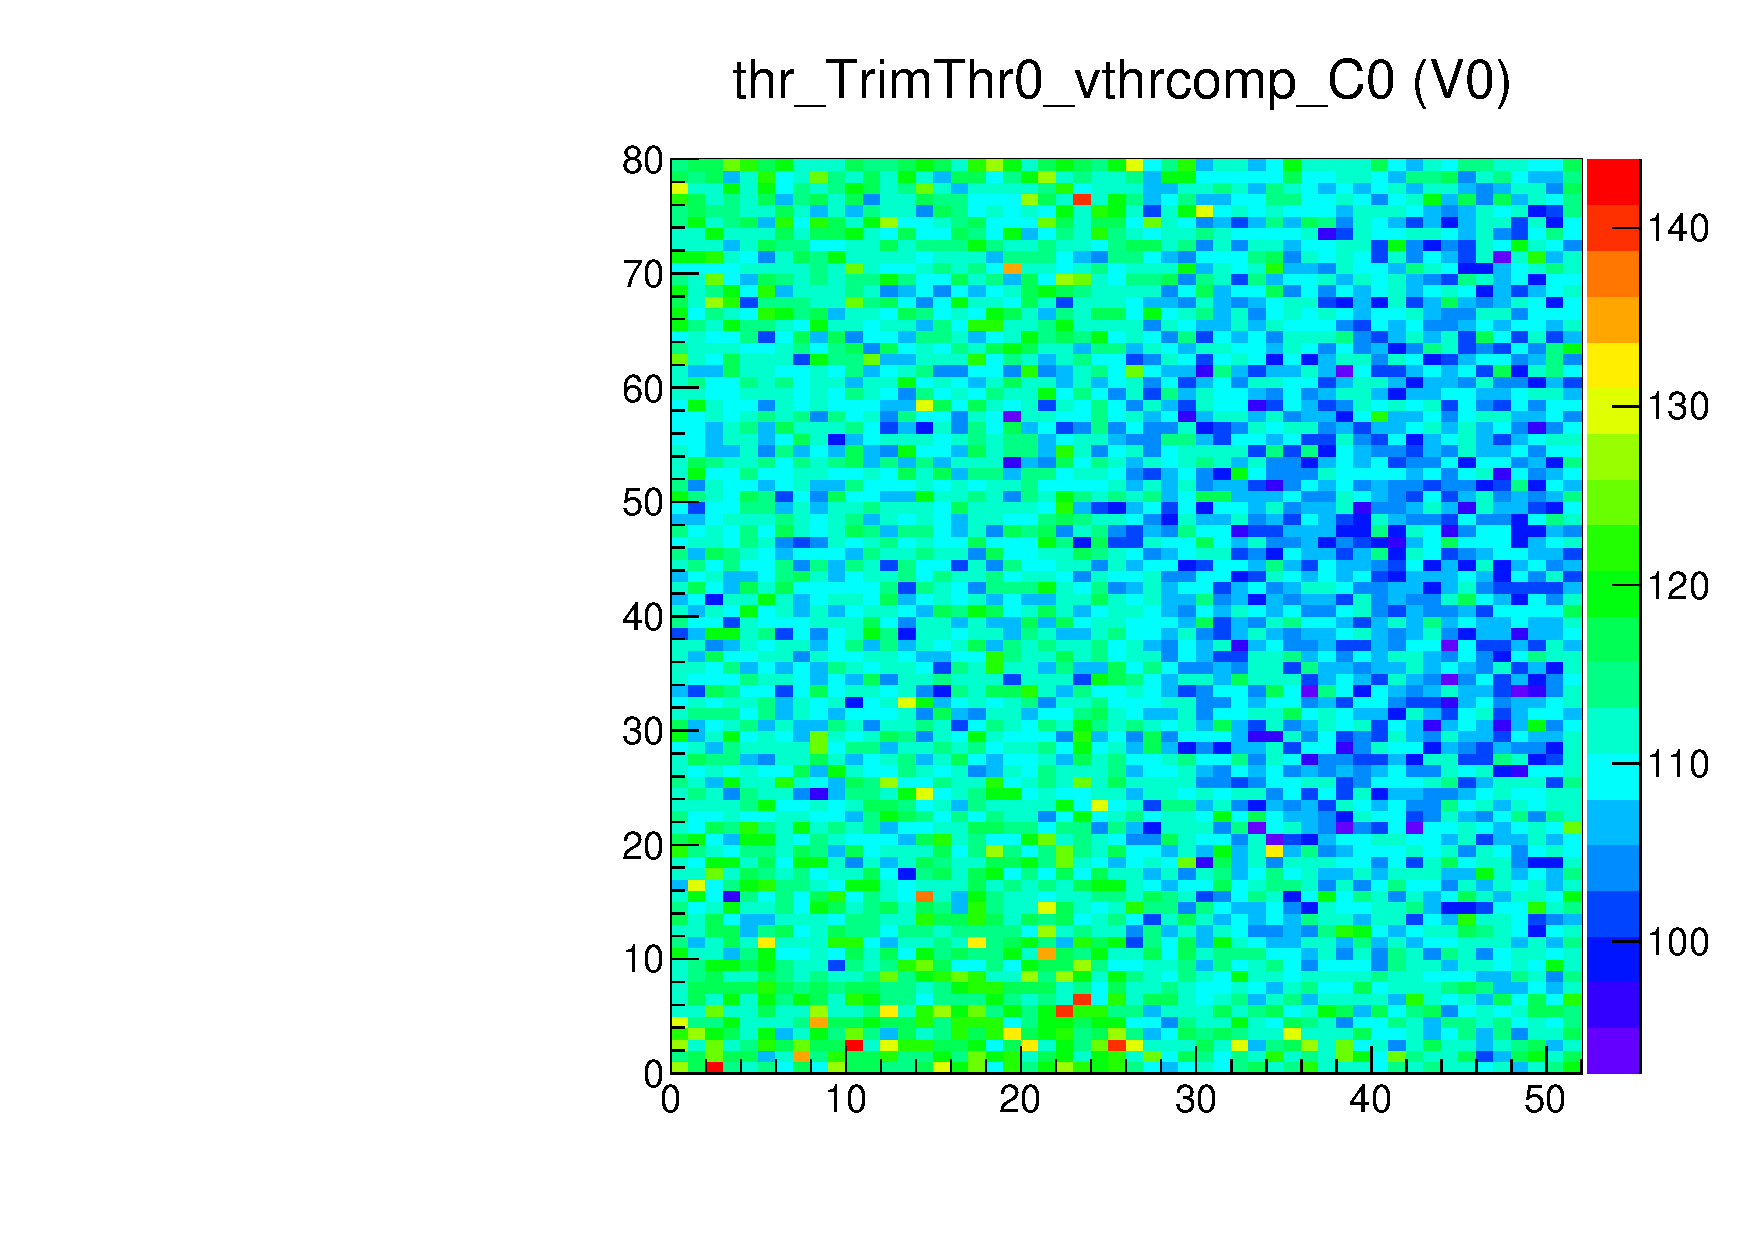
\includegraphics[width=1.0\textwidth]{figures/trim_thr_TrimThr0_vthrcomp.pdf}
  \caption{\roc map of \vthrcomp turn-on thresholds with \vcal set to target value.
           Used to find pixel with minimum turn-on (least sensitive pixel).}
  \label{fig:trim_thr_TrimThr0_vthrcomp}
\end{minipage}
\hspace{0.3cm}
\begin{minipage}{0.45\textwidth}

% from trim test:  scan to get maximal vcal turn-on pixel
  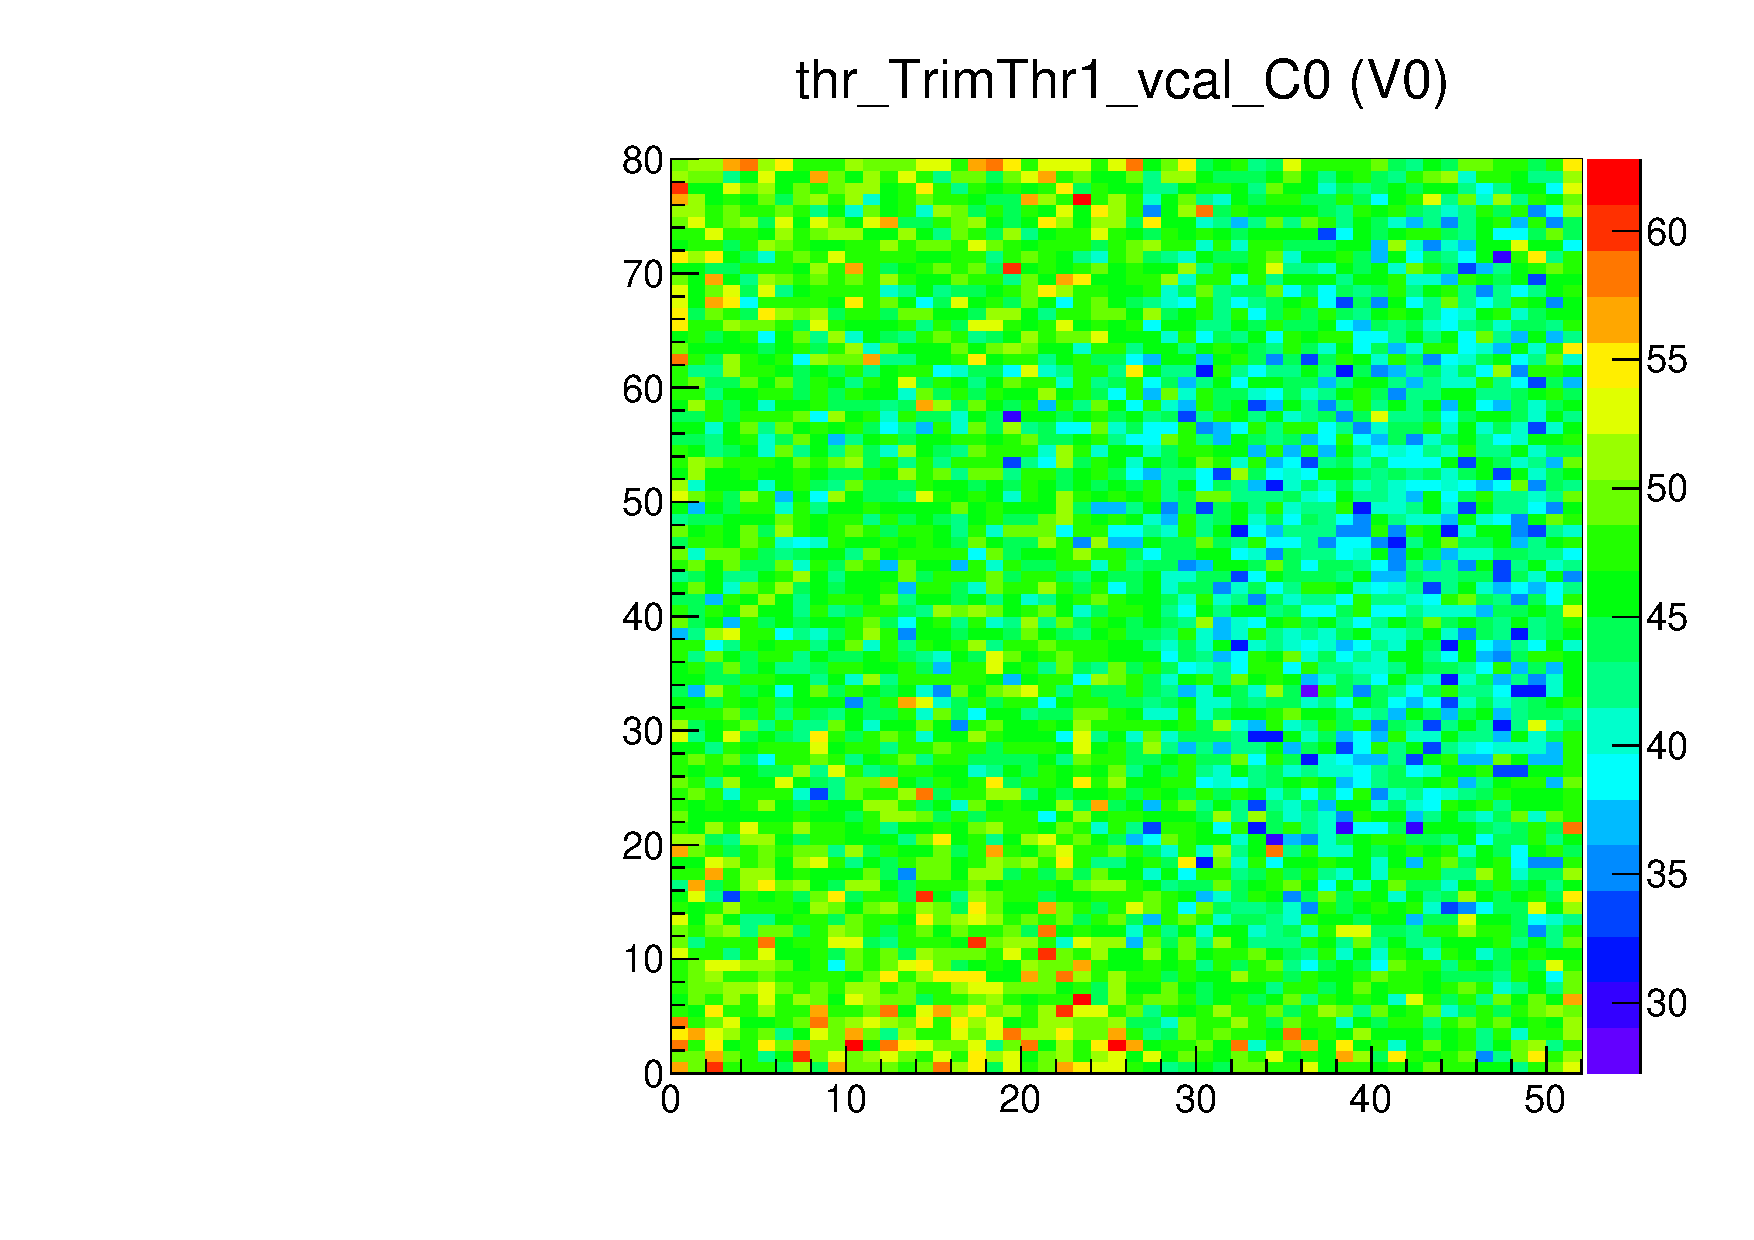
\includegraphics[width=1.0\textwidth]{figures/trim_thr_TrimThr1_vcal.pdf}
  \caption{\roc map of \vcal turn-on thresholds with minimized \vthrcomp value.  
           Used to find most sensitive pixel, i.e. the pixel requiring maximum trimming.}
  \label{fig:trim_thr_TrimThr1_vcal}
\end{minipage}
\end{figure}

% from trim test: efficiency in vcal/trim plane, for setting Vtrim

\begin{figure}[!htp]
\centering
\begin{minipage}{0.45\textwidth}
  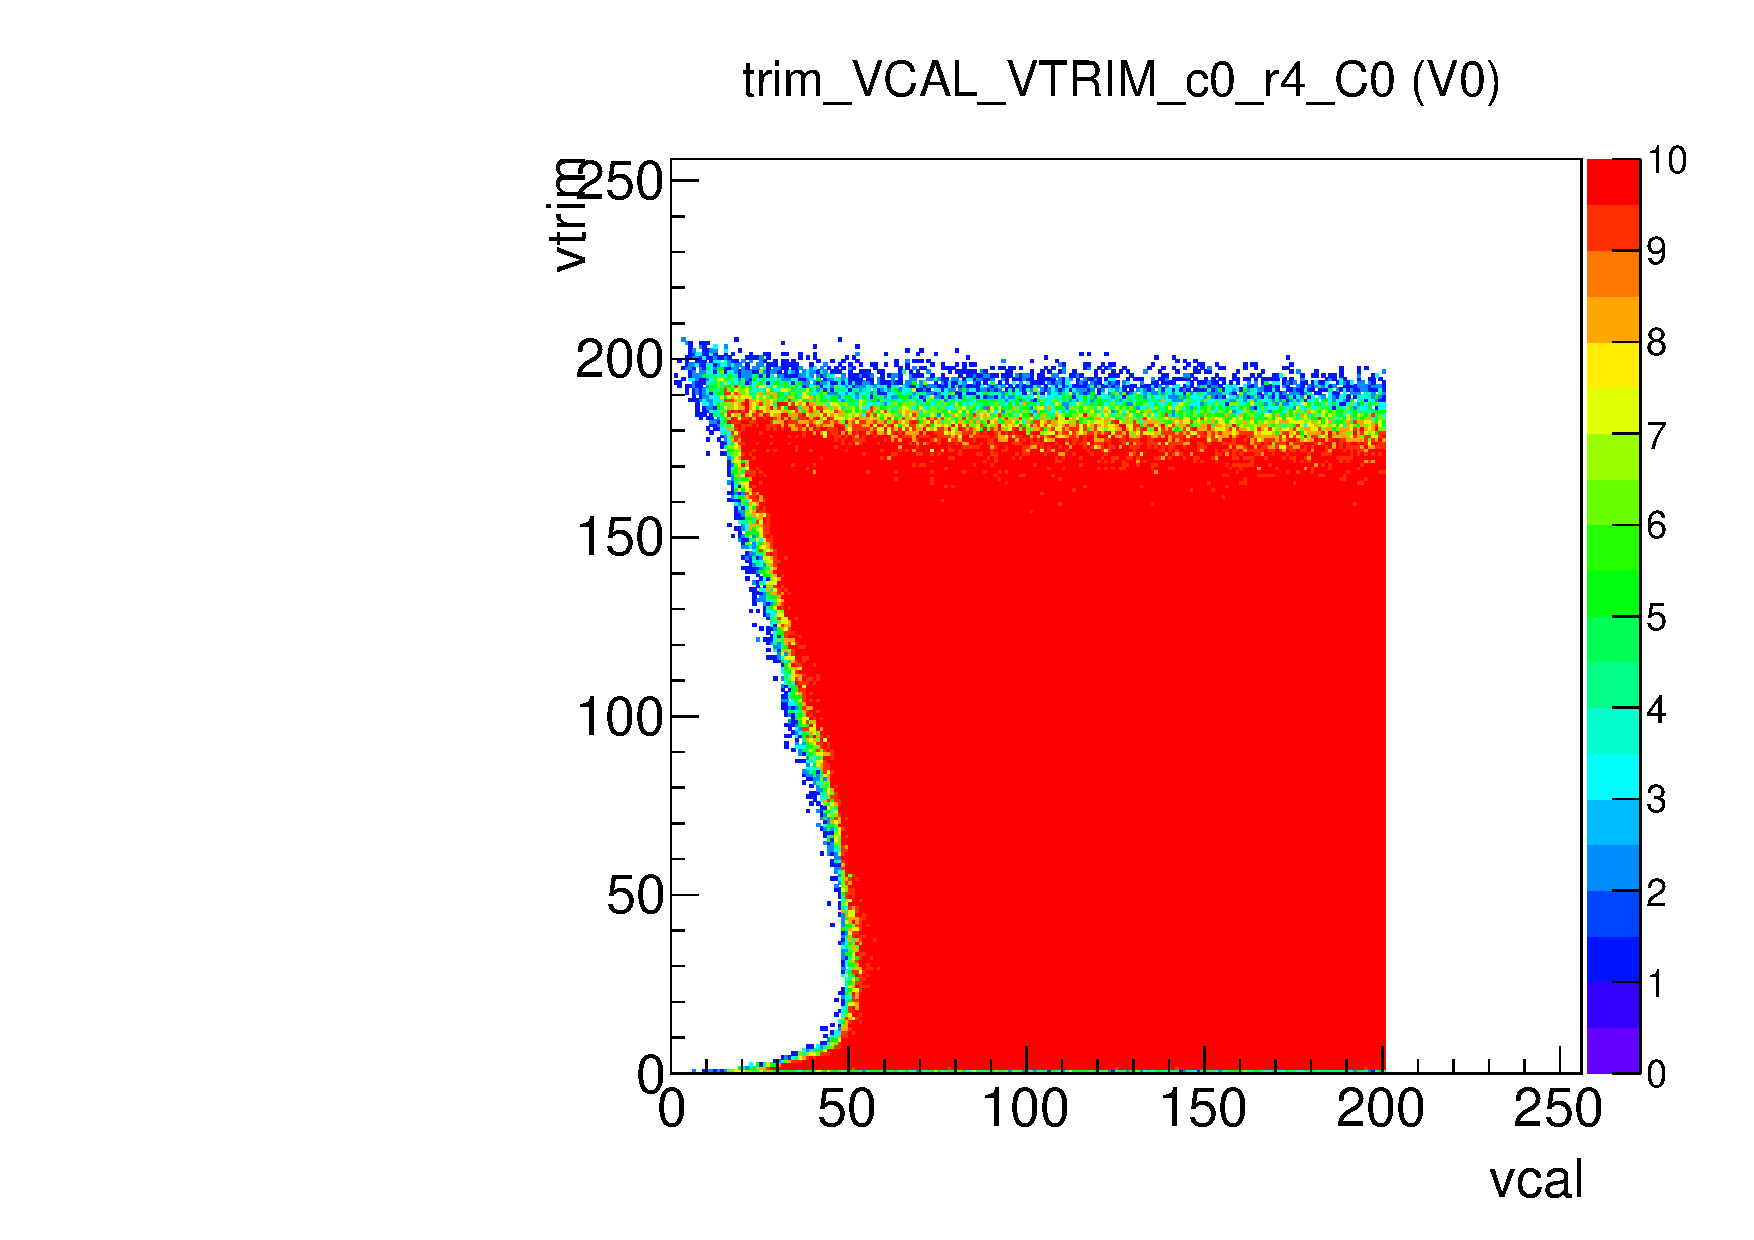
\includegraphics[width=1.0\textwidth]{figures/trim_trim_VCAL_VTRIM.pdf}
  \caption{Efficiency in the \vtrim vs. \vcal plane.
           Used to find the value of \vtrim that corresponds to a turn-on at the target \vcal.}
  \label{fig:trim_trim_VCAL_VTRIM}
\end{minipage}
\end{figure}

% from trim test: threshold maps after each iteration of trim correction

\begin{figure}[!htp]
\centering
\begin{minipage}{0.45\textwidth}
  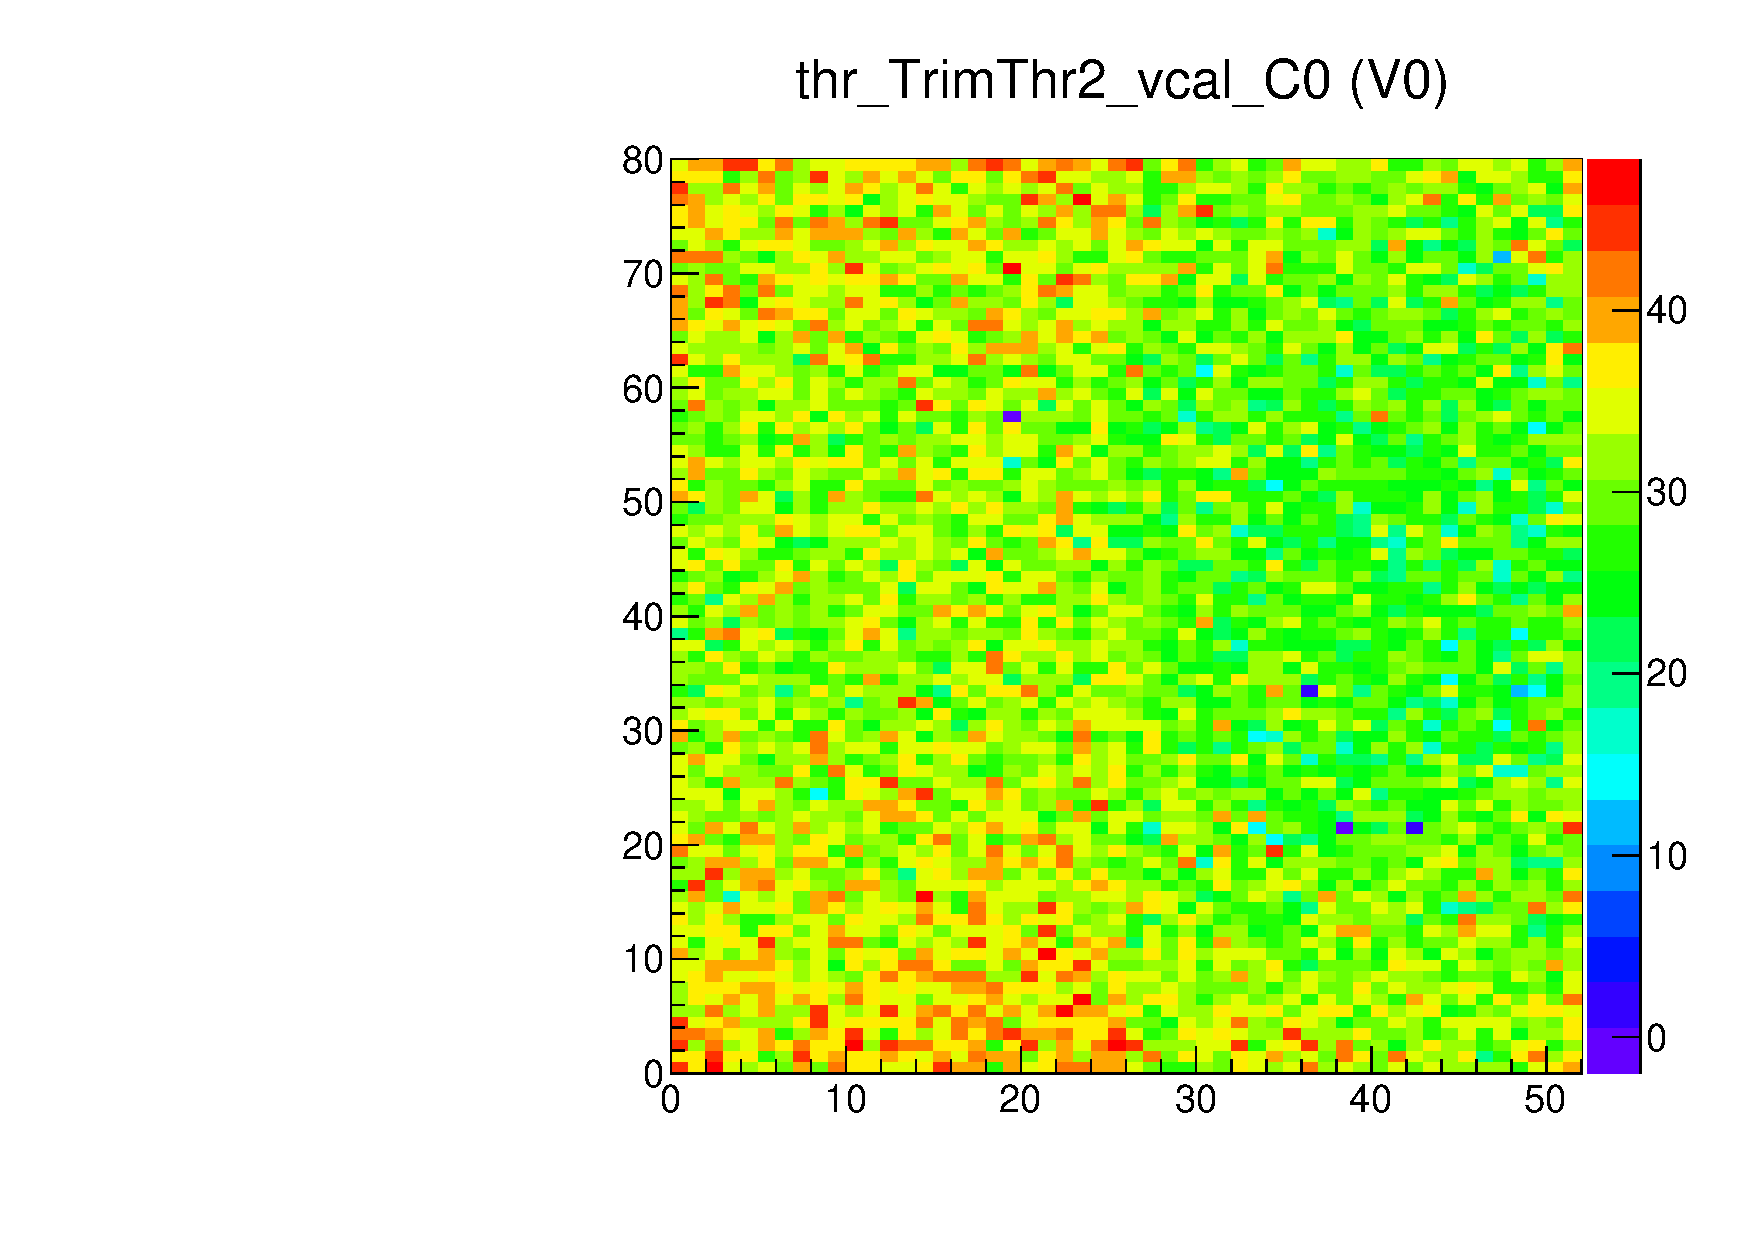
\includegraphics[width=1.0\textwidth]{figures/trim_thr_TrimThr2_vcal.pdf}
  \caption{\roc map of \vcal turn-on thresholds with \trimbits=7.
           Used as baseline for setting the \trimbits.}
  \label{fig:trim_thr_TrimThr2_vcal}
\end{minipage}
\end{figure}

\begin{figure}[!htp]
\centering
\begin{minipage}{0.45\textwidth}
  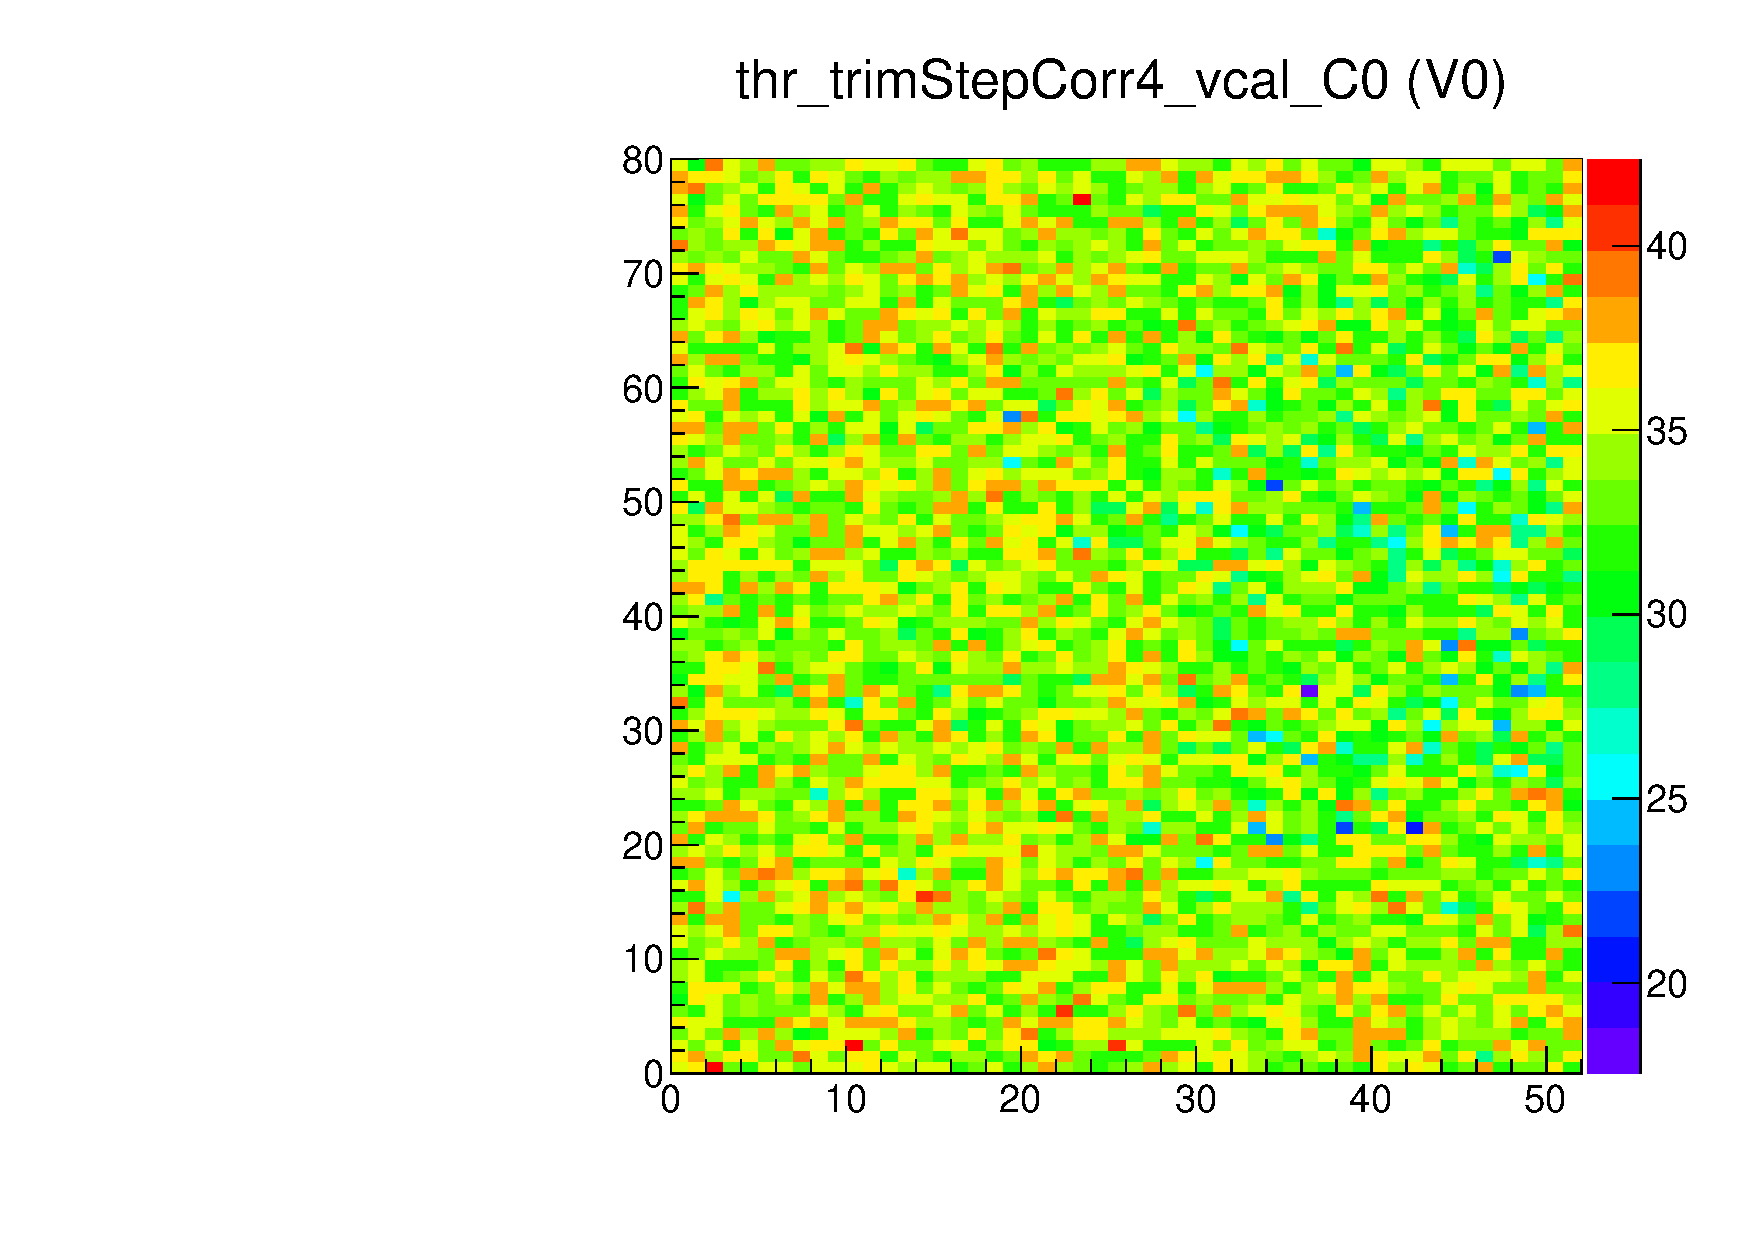
\includegraphics[width=1.0\textwidth]{figures/trim_thr_trimStepCorr4_vcal.pdf}
  \caption{\roc map of \vcal turn-on thresholds after a \trimbits$\pm$4 correction with respect to Figure~\ref{fig:trim_thr_TrimThr2_vcal}.}
  \label{fig:trim_thr_trimStepCorr4_vcal}
\end{minipage}
\hspace{0.3cm}
\begin{minipage}{0.45\textwidth}
  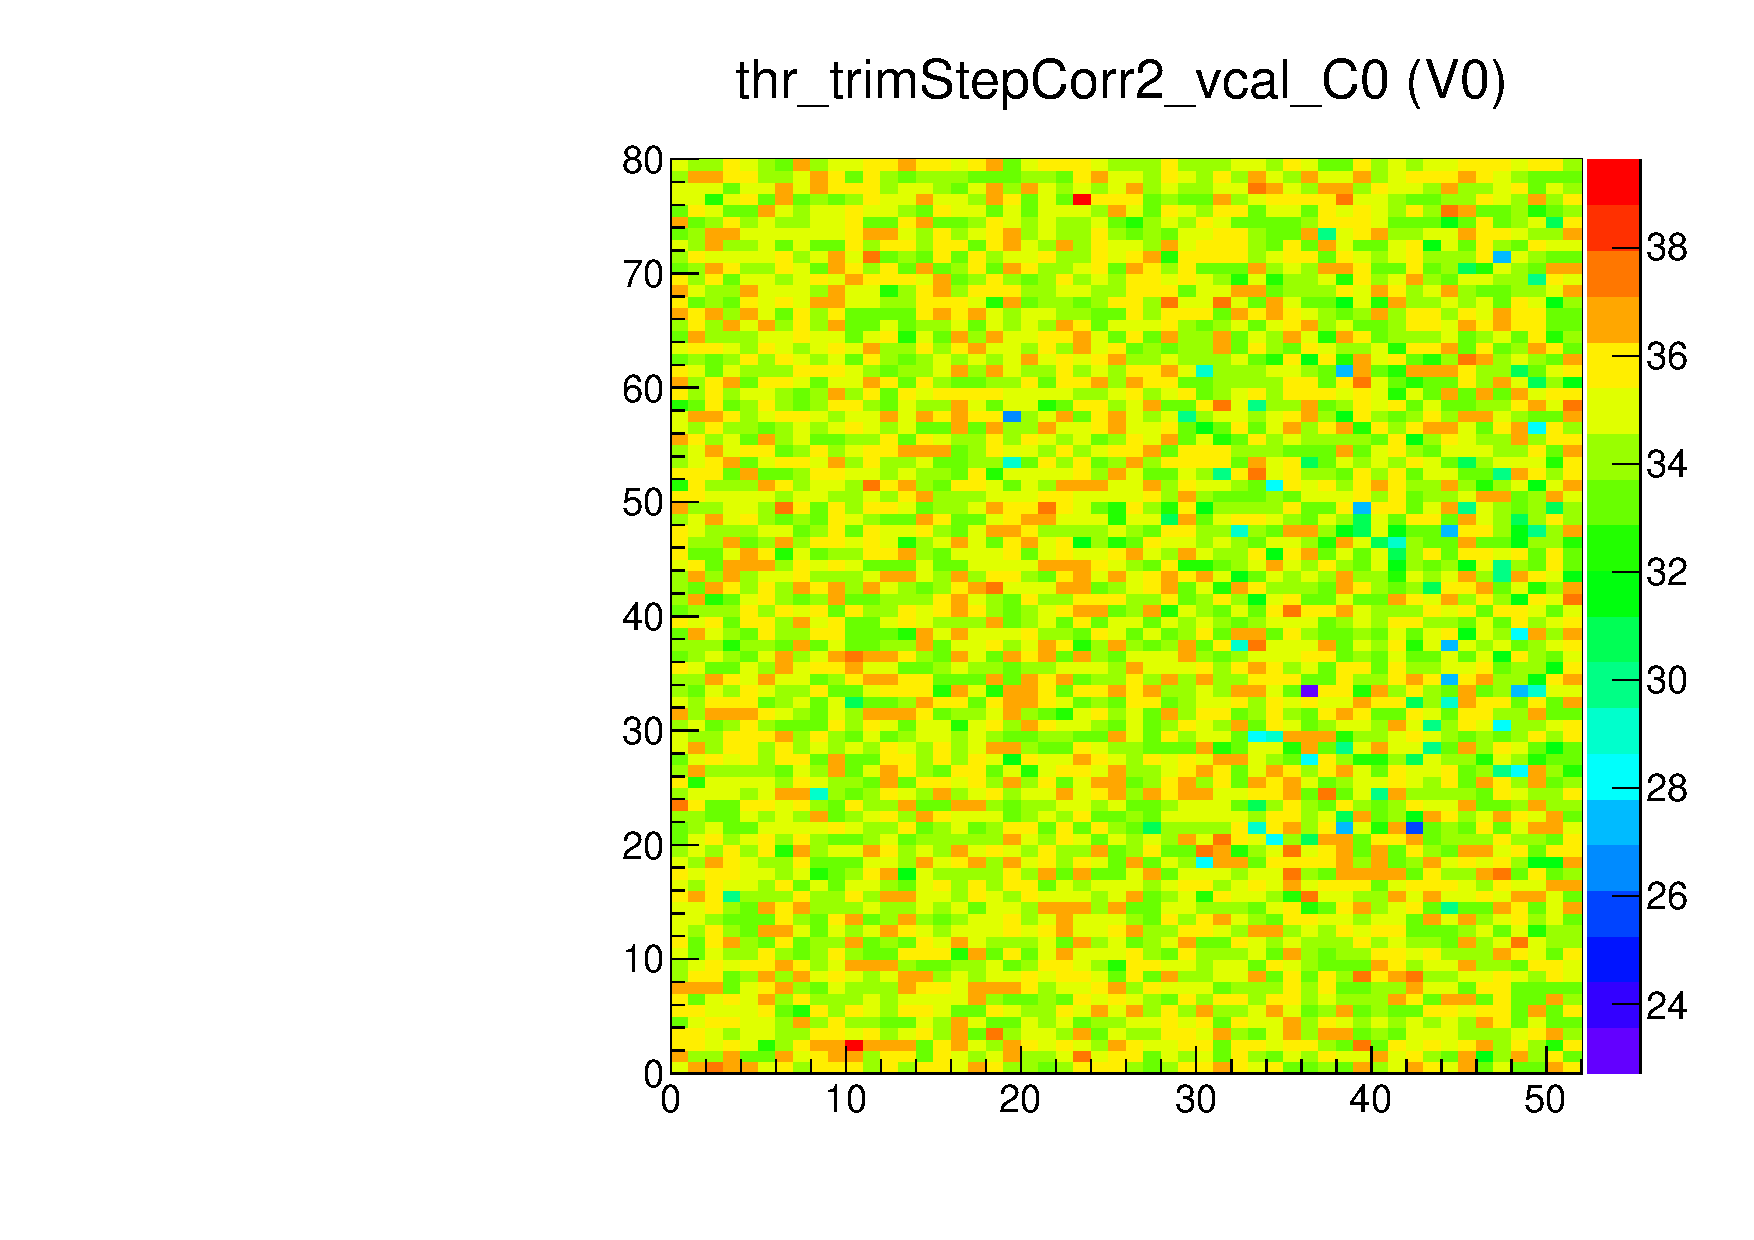
\includegraphics[width=1.0\textwidth]{figures/trim_thr_trimStepCorr2_vcal.pdf}
  \caption{\roc map of \vcal turn-on thresholds after a \trimbits$\pm$2 correction with respect to Figure~\ref{fig:trim_thr_trimStepCorr4_vcal}.}
  \label{fig:trim_thr_trimStepCorr2_vcal}
\end{minipage}
\end{figure}

\begin{figure}[!htp]
\centering
\begin{minipage}{0.45\textwidth}
  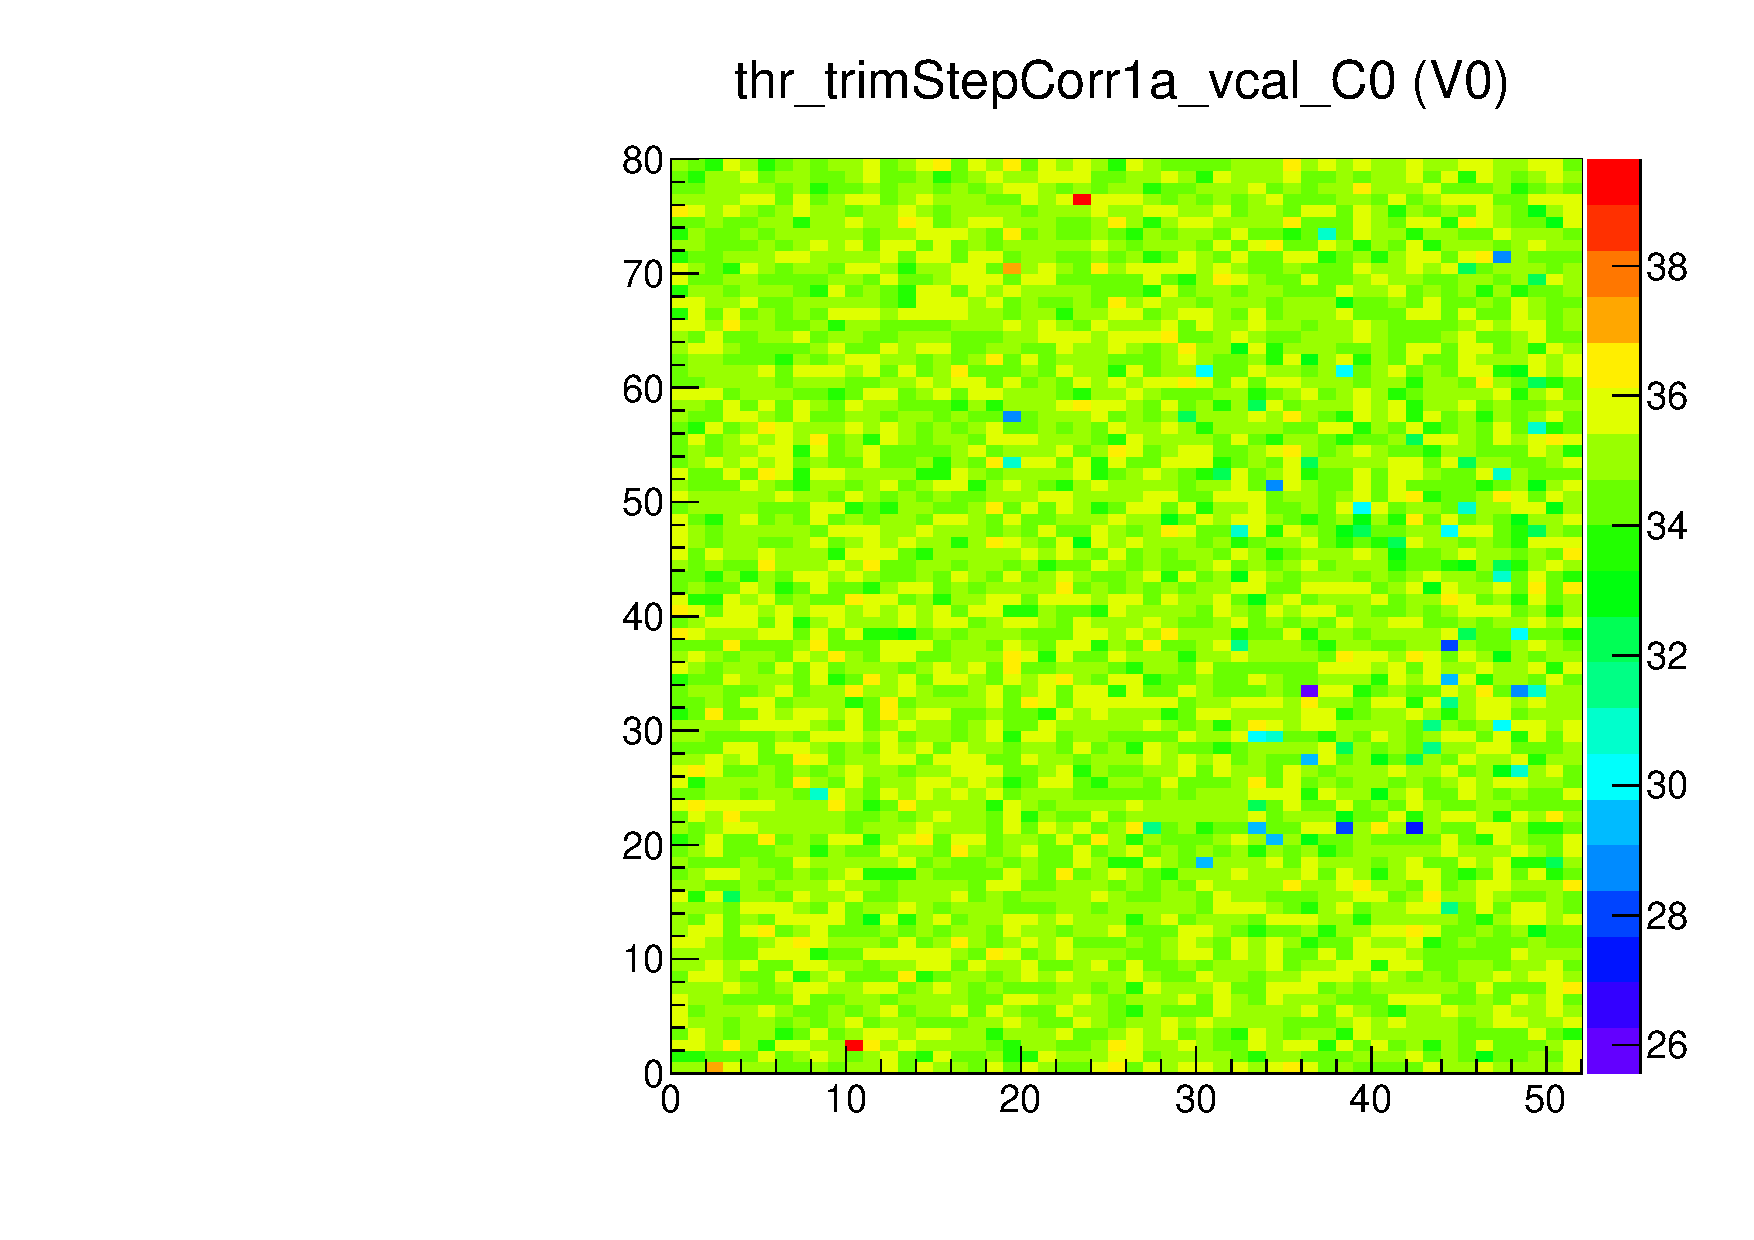
\includegraphics[width=1.0\textwidth]{figures/trim_thr_trimStepCorr1a_vcal.pdf}
  \caption{\roc map of \vcal turn-on thresholds after a \trimbits$\pm$1 correction with respect to Figure~\ref{fig:trim_thr_trimStepCorr2_vcal}.}
  \label{fig:trim_thr_trimStepCorr1a_vcal}
\end{minipage}
\hspace{0.3cm}
\begin{minipage}{0.45\textwidth}
  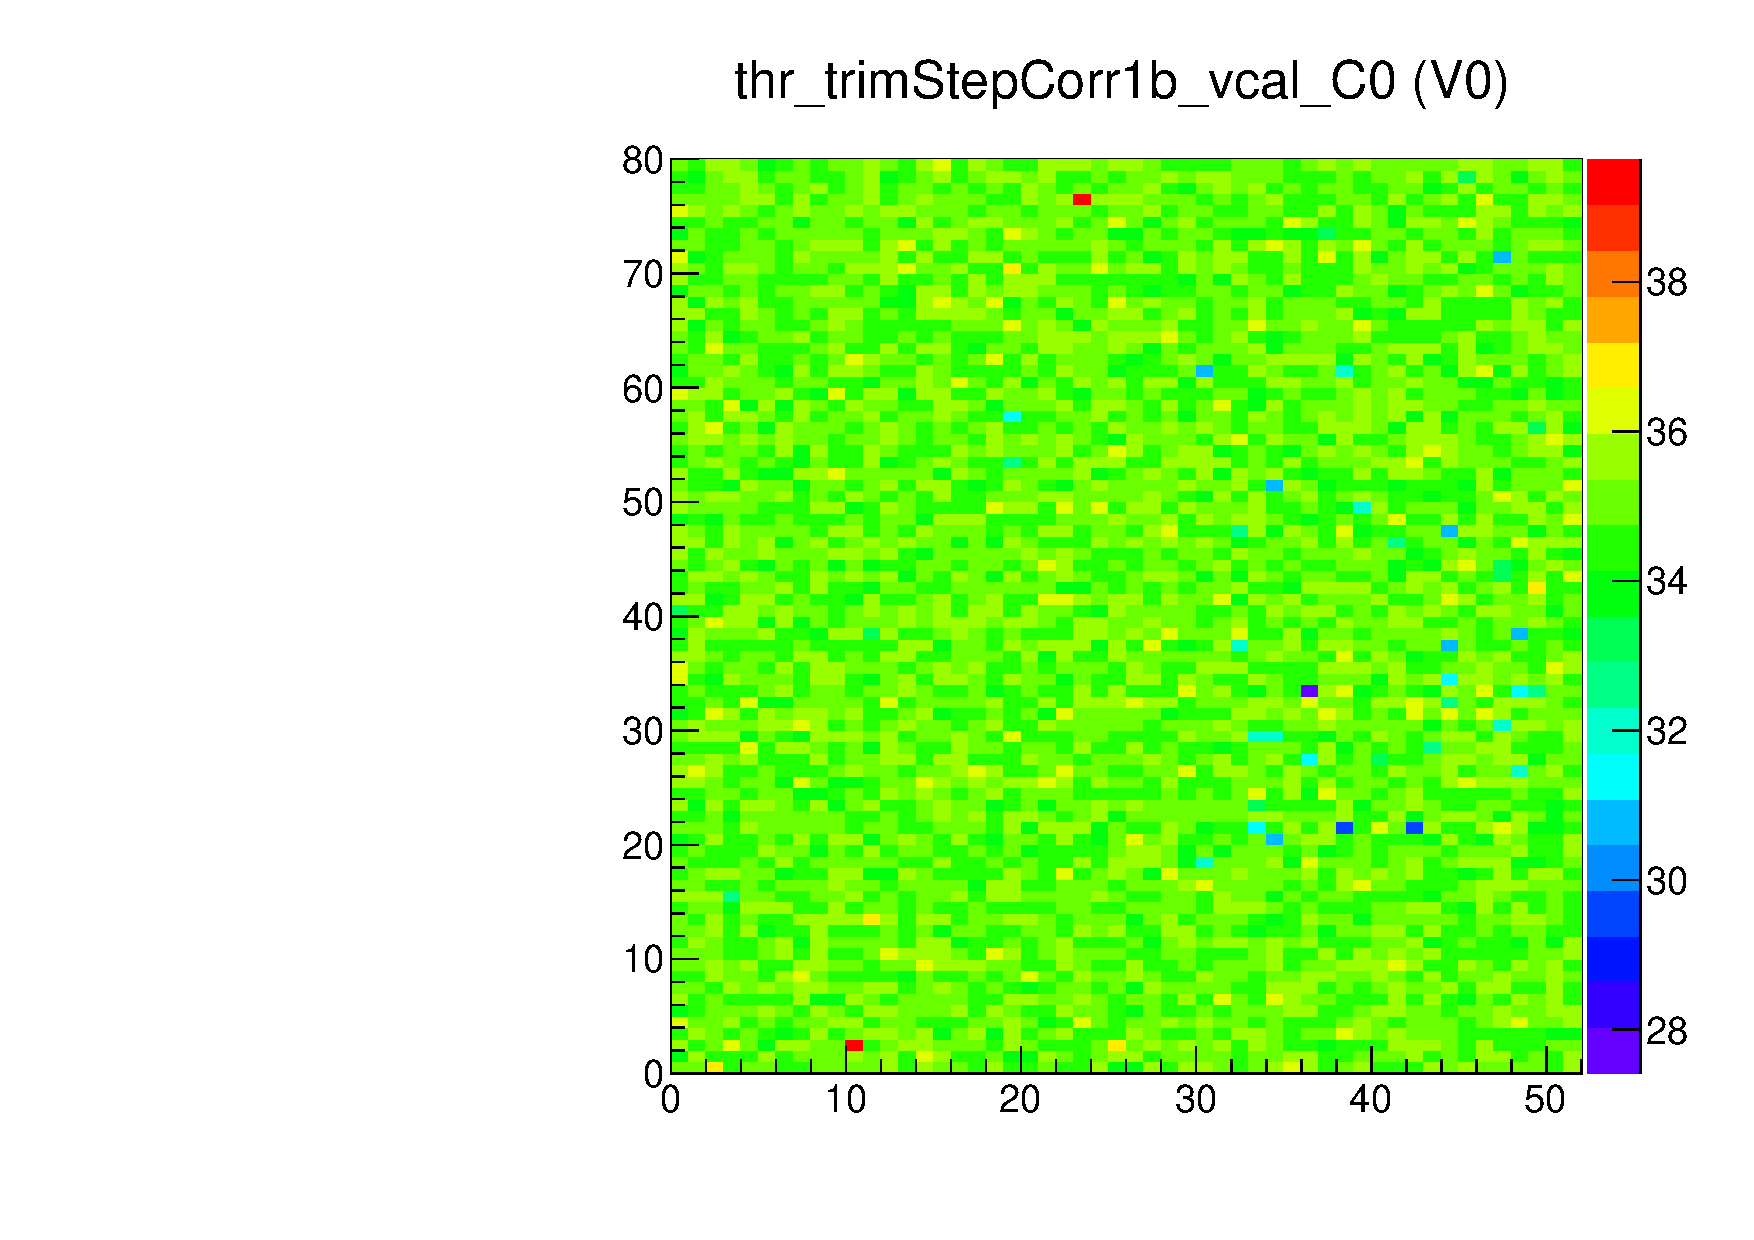
\includegraphics[width=1.0\textwidth]{figures/trim_thr_trimStepCorr1b_vcal.pdf}
  \caption{\roc map of \vcal turn-on thresholds after a \trimbits$\pm$1 correction with respect to Figure~\ref{fig:trim_thr_trimStepCorr1a_vcal}.}
  \label{fig:trim_thr_trimStepCorr1b_vcal}
\end{minipage}
\end{figure}


% from trim test:  optimized trim bits

\begin{figure}[!htp]
\centering
\begin{minipage}{0.45\textwidth}
  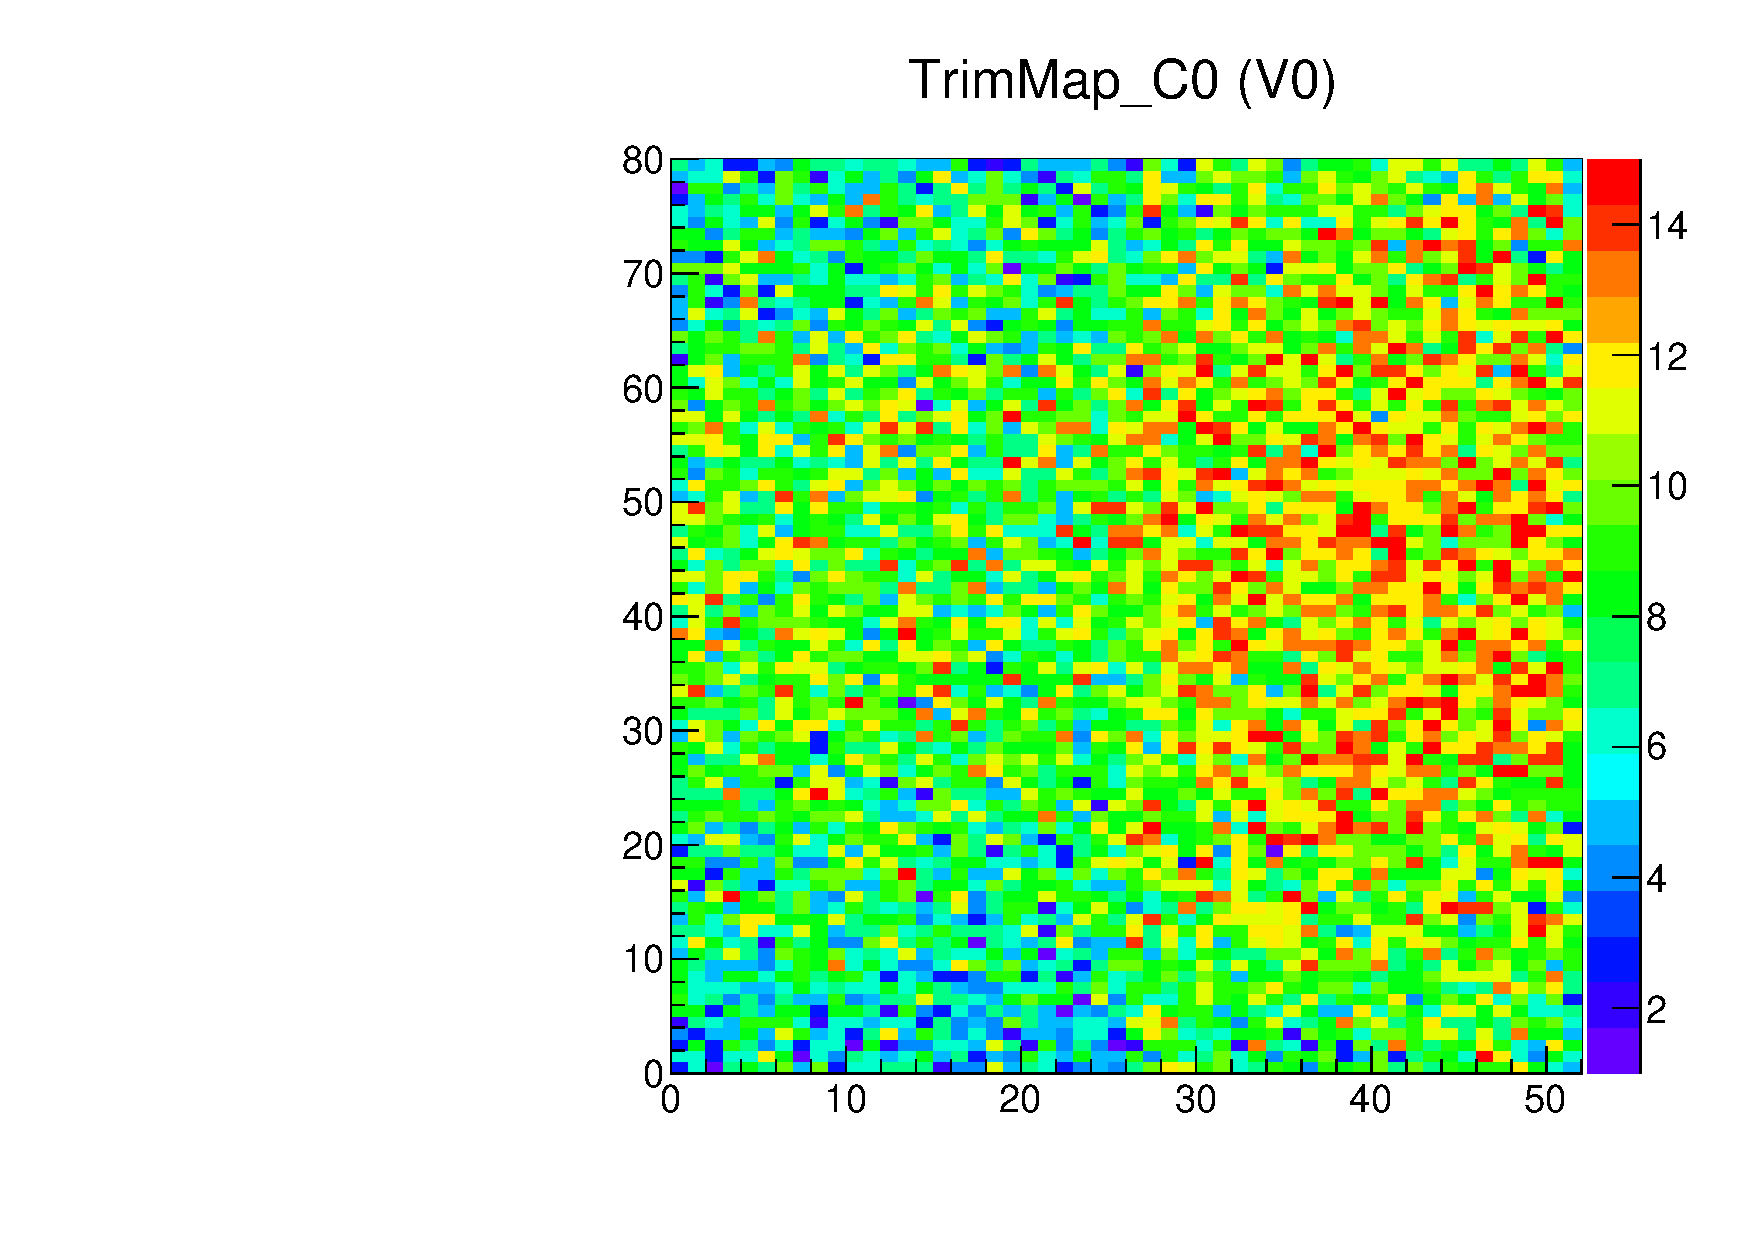
\includegraphics[width=1.0\textwidth]{figures/trim_TrimMap.pdf}
  \caption{\roc map of the optimized trim bit values (0-15).}
  \label{fig:trim_TrimMap}
\end{minipage}
\hspace{0.3cm}
\begin{minipage}{0.45\textwidth}
  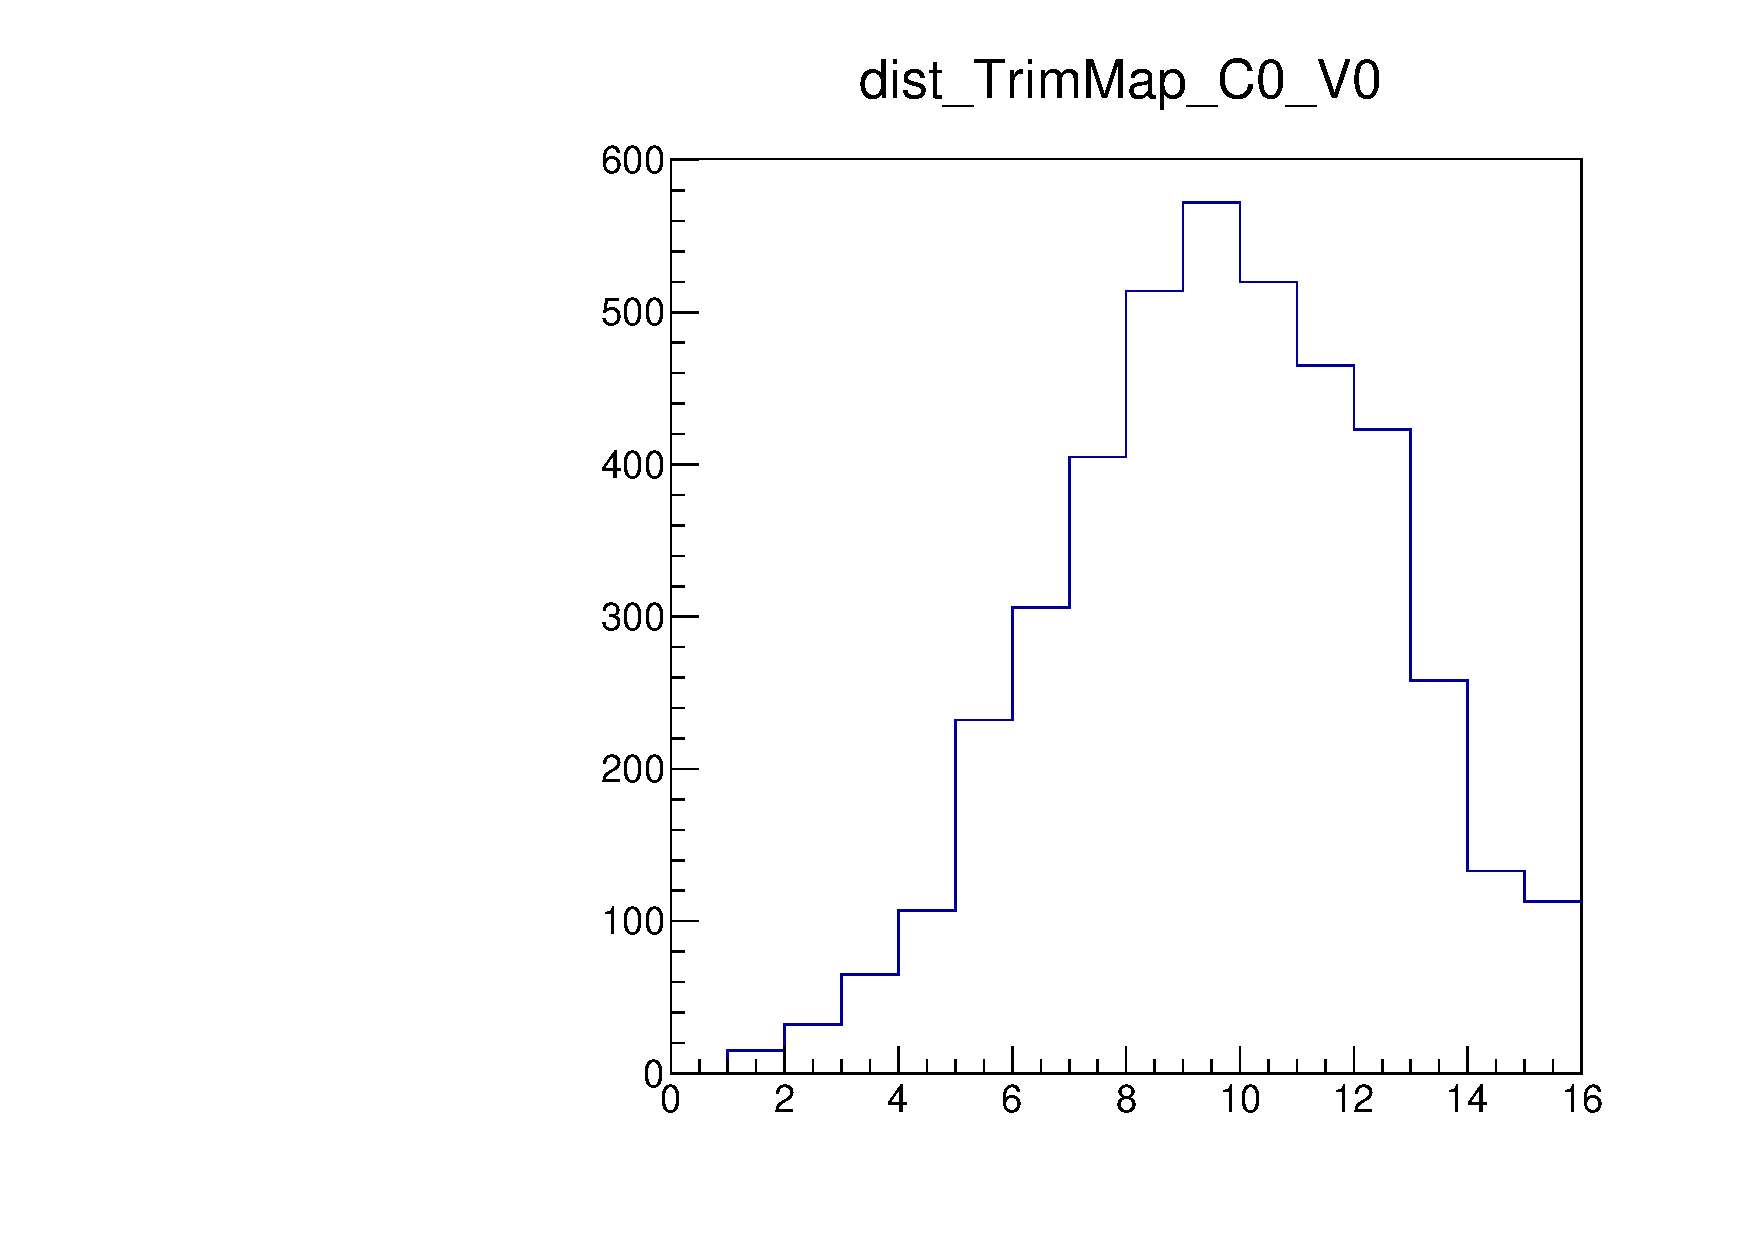
\includegraphics[width=1.0\textwidth]{figures/trim_dist_TrimMap.pdf}
  \caption{1D distribution of the optimized trim bit values (0-15).}
  \label{fig:trim_dist_TrimMap}
\end{minipage}
\end{figure}

% from trim test: vcal turn-on after trimming

\begin{figure}[!htp]
\centering
\begin{minipage}{0.45\textwidth}
  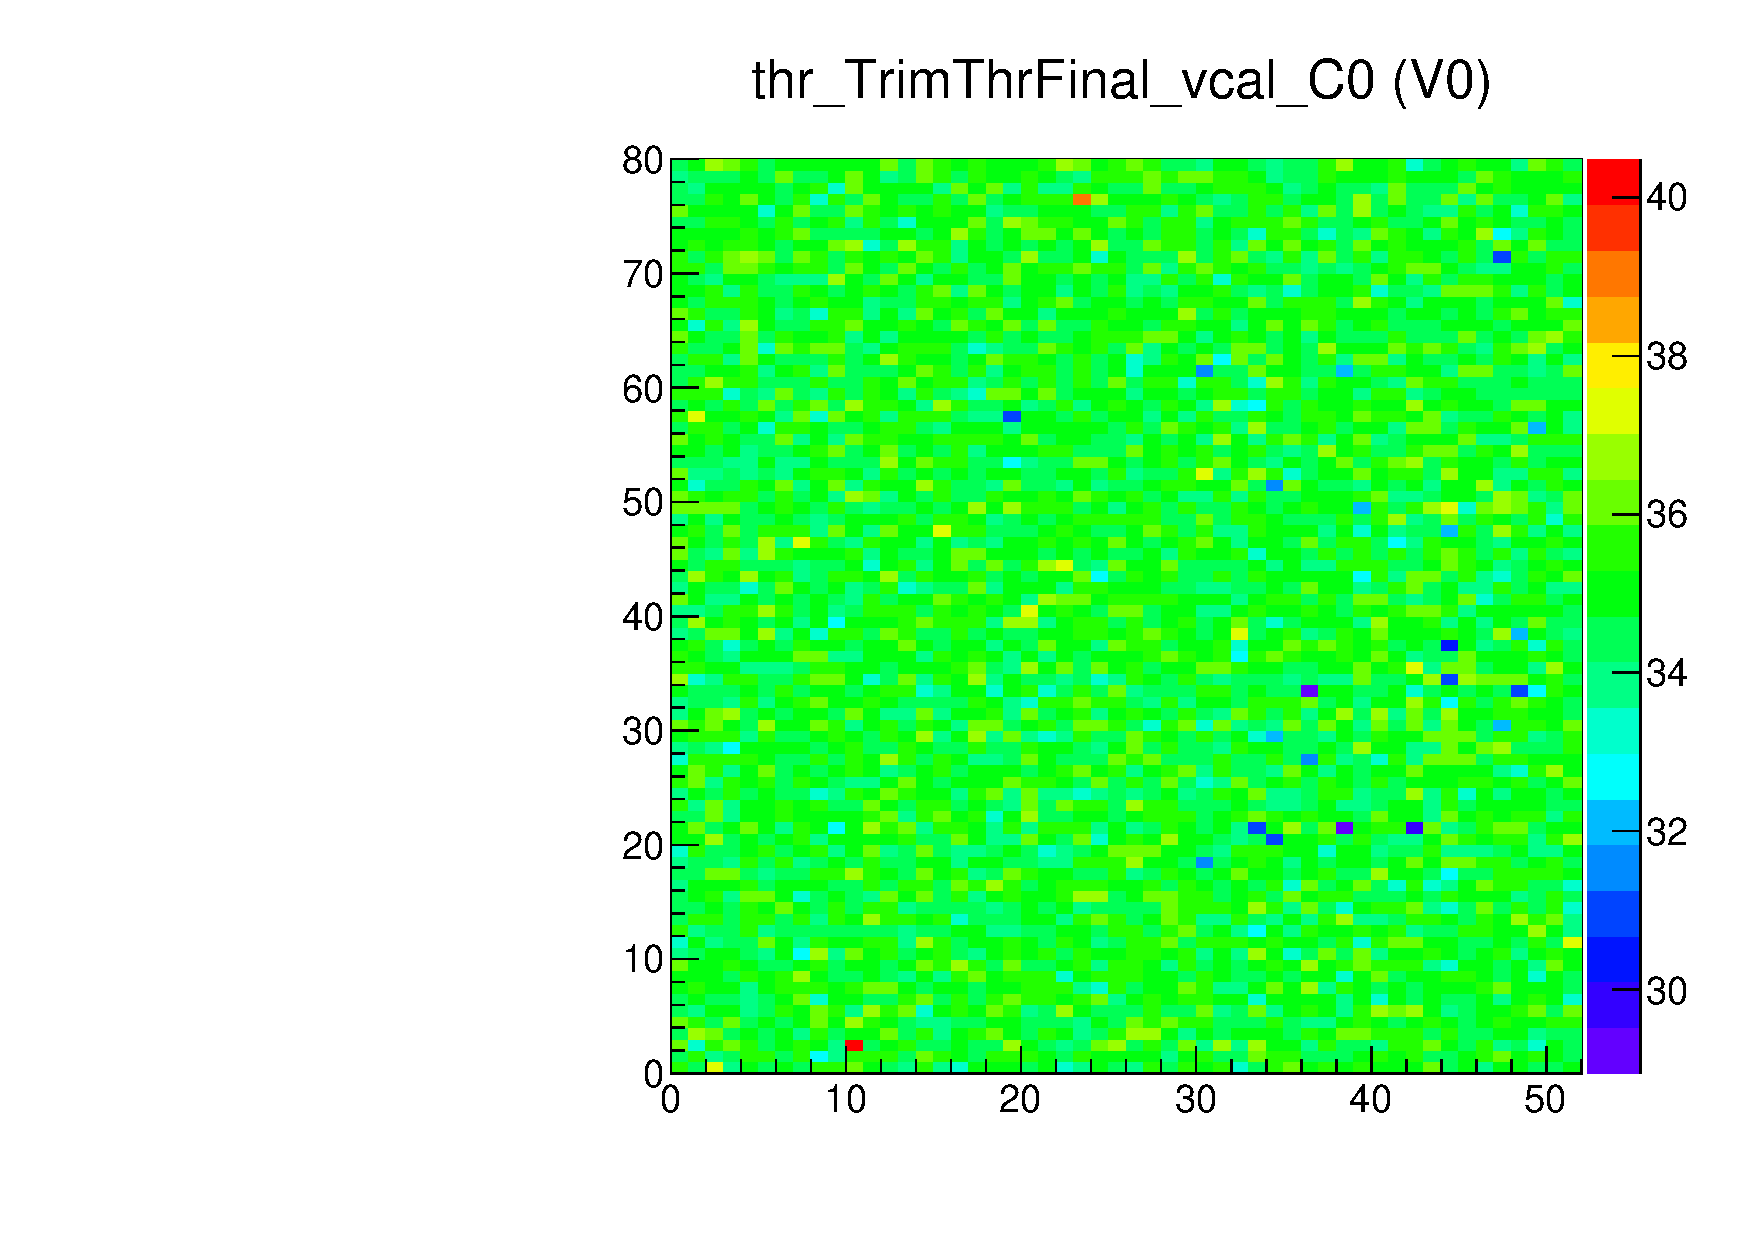
\includegraphics[width=1.0\textwidth]{figures/trim_thr_TrimThrFinal_vcal.pdf}
  \caption{\roc map of the \vcal turn-on thresholds with optimized trim parameters.}
  \label{fig:trim_thr_TrimThrFinal_vcal}
\end{minipage}
\hspace{0.3cm}
\begin{minipage}{0.45\textwidth}
  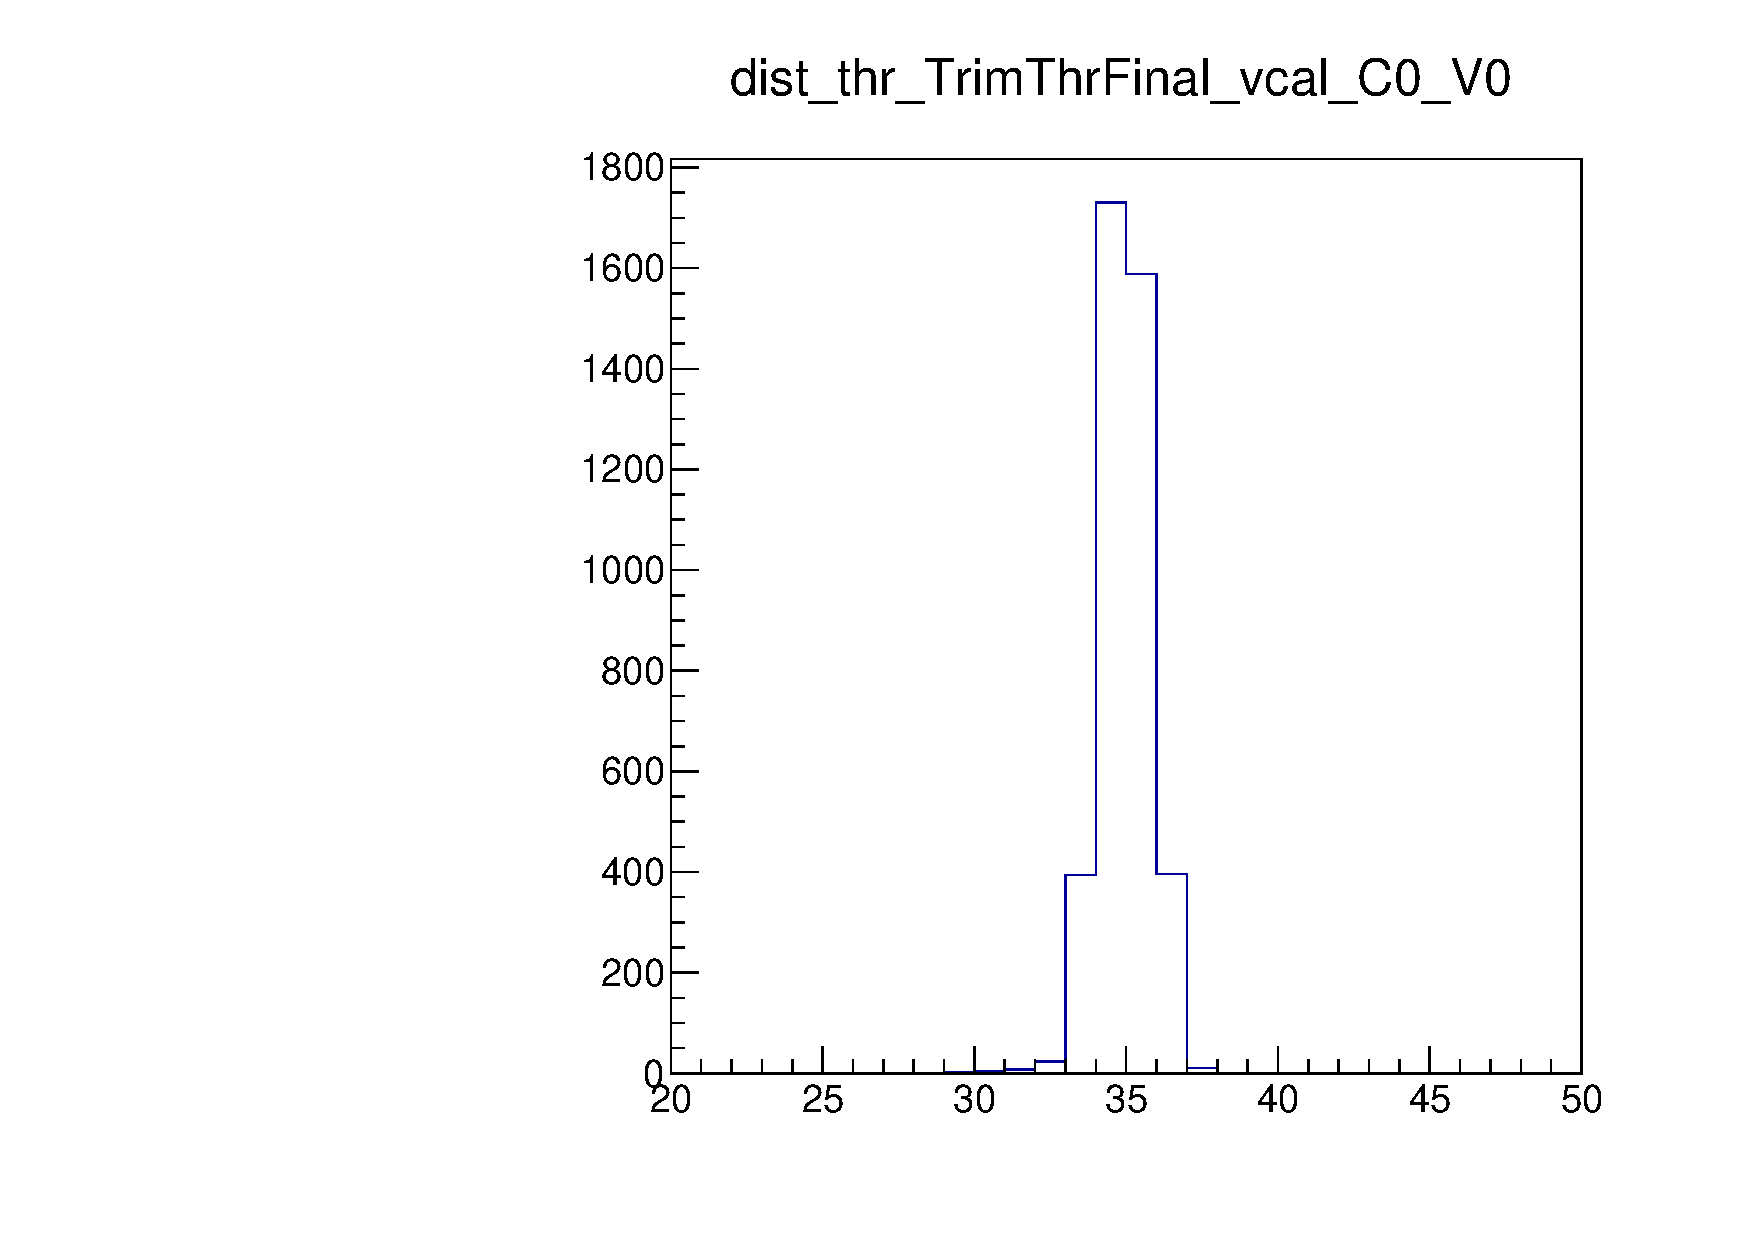
\includegraphics[width=1.0\textwidth]{figures/trim_dist_thr_TrimThrFinal_vcal.pdf}
  \caption{1D distribution of the \vcal turn-on thresholds with optimized trim parameters. [original range 0-255]}
  \label{fig:trim_dist_thr_TrimThrFinal_vcal}
\end{minipage}
\end{figure}


% ---------------------------------------------------------------------


% from trim bit test: untrimmed thresholds (trim bits = 15)

\begin{figure}[!htp]
\centering
\begin{minipage}{0.45\textwidth}
  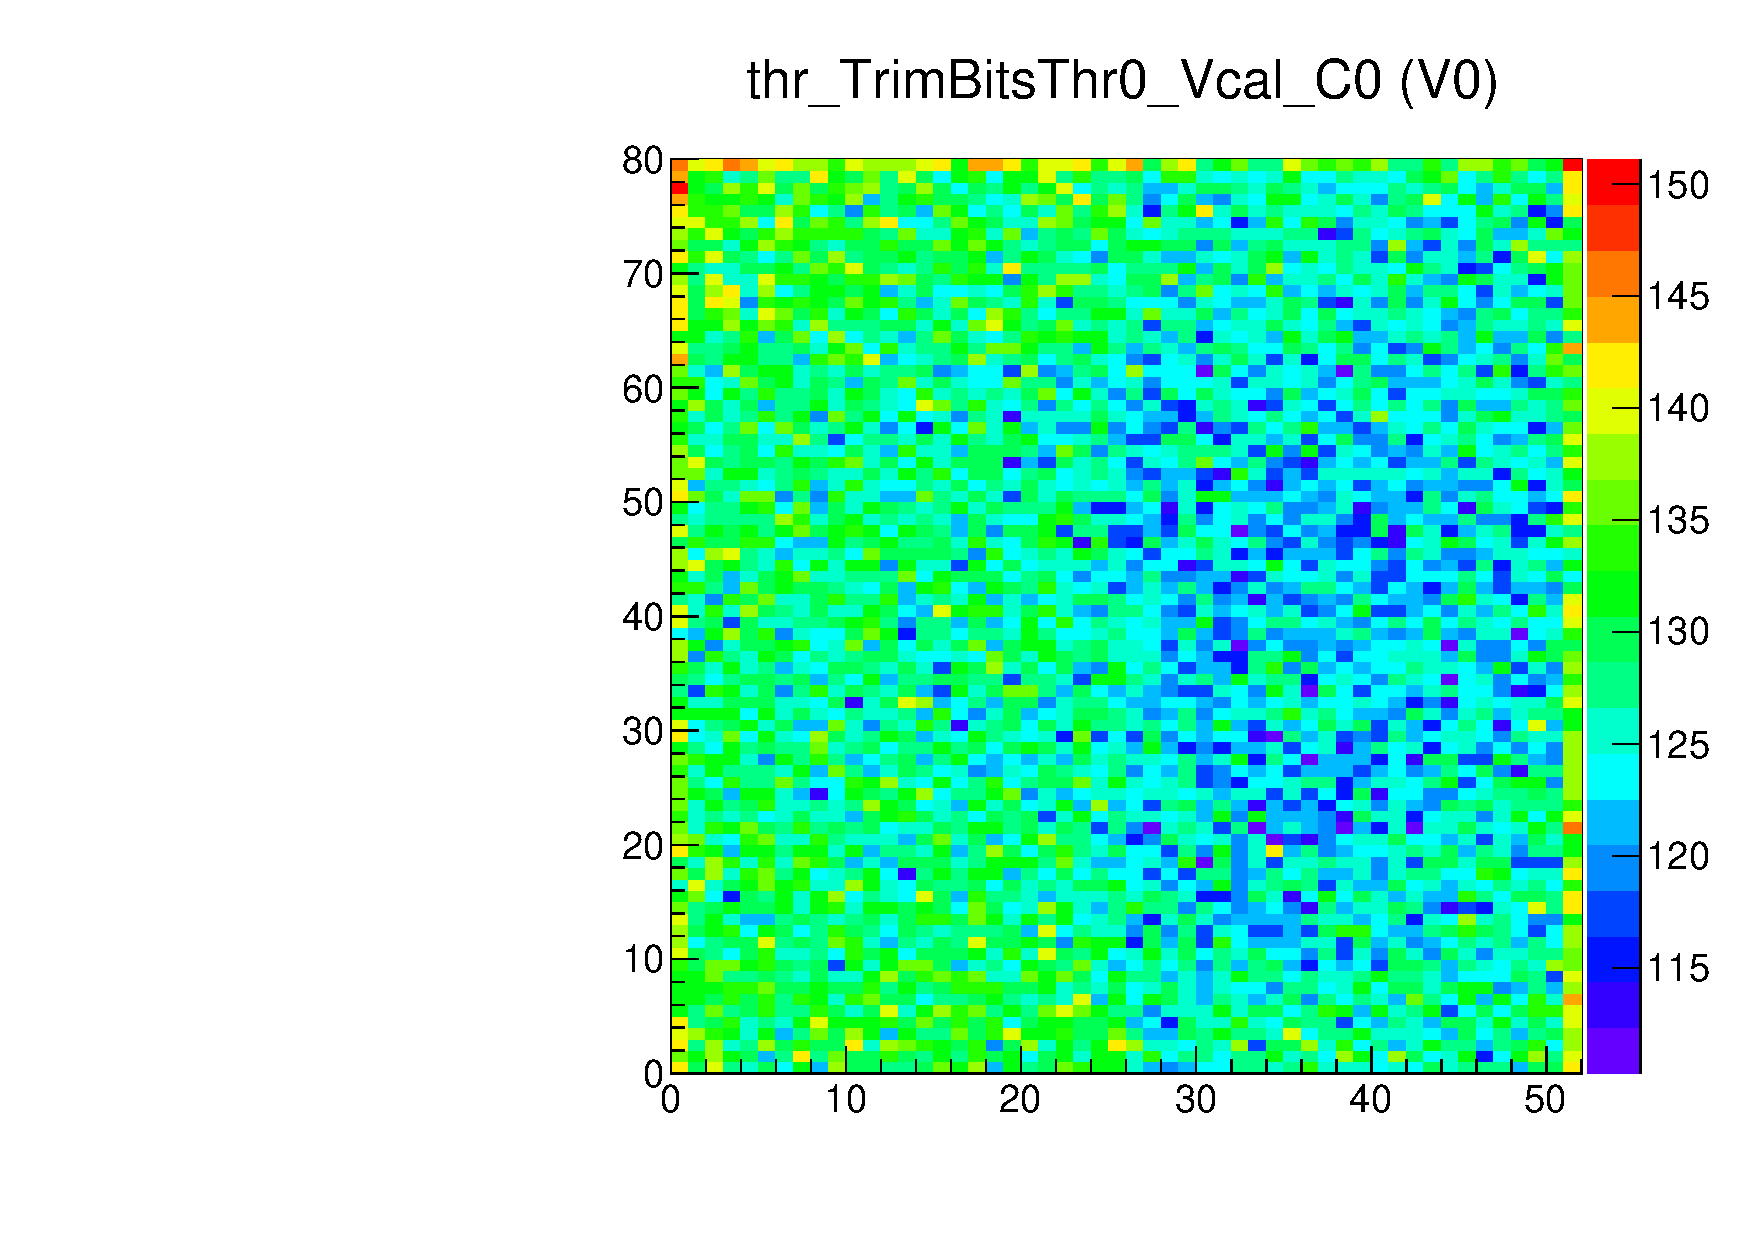
\includegraphics[width=1.0\textwidth]{figures/trim_thr_TrimBitsThr0_Vcal.pdf}
  \caption{\roc map of untrimmed \vcal thresholds.
           Used as a baseline for the \trimbit test.}
  \label{fig:trim_thr_TrimBitsThr0_Vcal}
\end{minipage}
\end{figure}


% from trim bits test:  vcal thresholds for different trim bit values trim_thr_TrimThr

\begin{figure}[!htp]
\centering
\begin{minipage}{0.45\textwidth}
  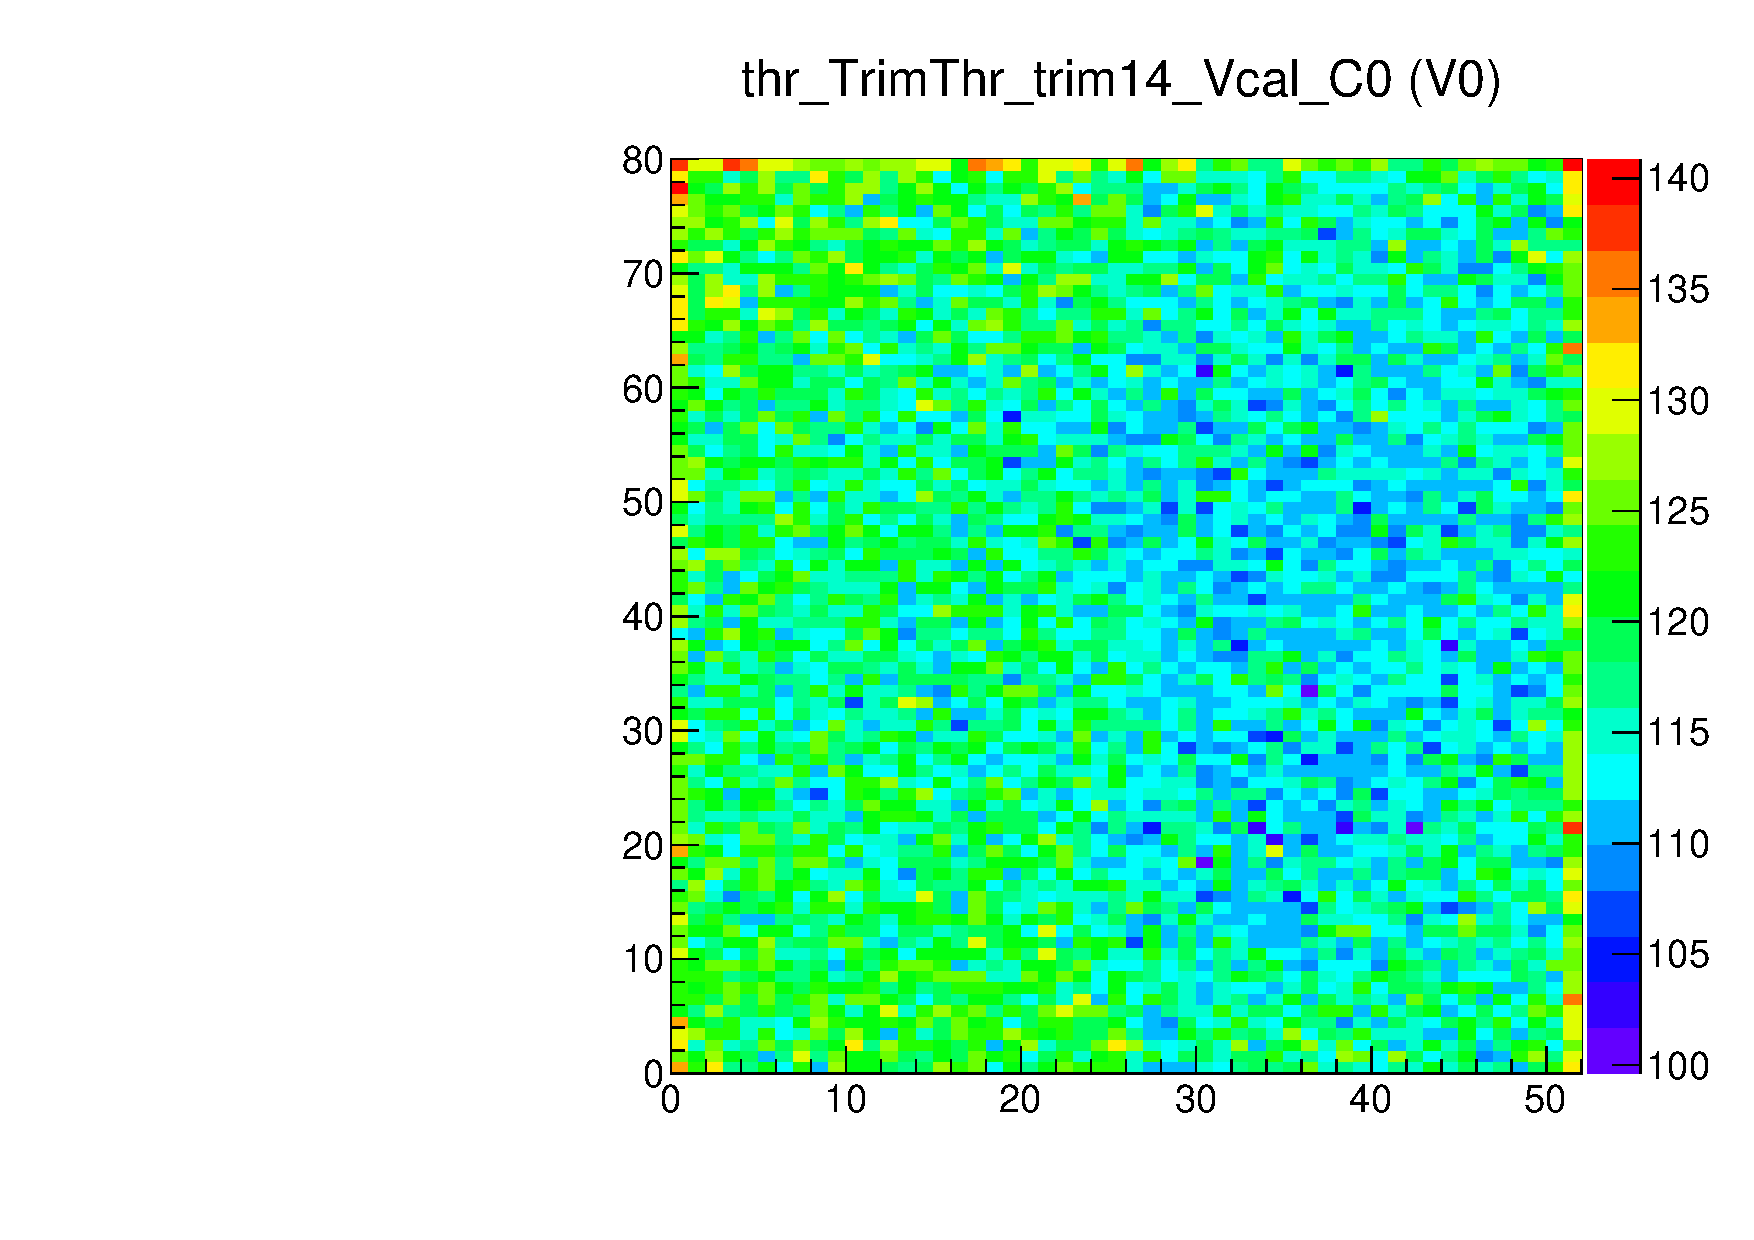
\includegraphics[width=1.0\textwidth]{figures/trim_thr_TrimThr_trim14_Vcal.pdf}
  \caption{\roc map of \vcal thresholds with \trimbits=14 [1110].}
  \label{fig:trim_thr_TrimThr_trim14_Vcal}
\end{minipage}
\hspace{0.3cm}
\begin{minipage}{0.45\textwidth}
  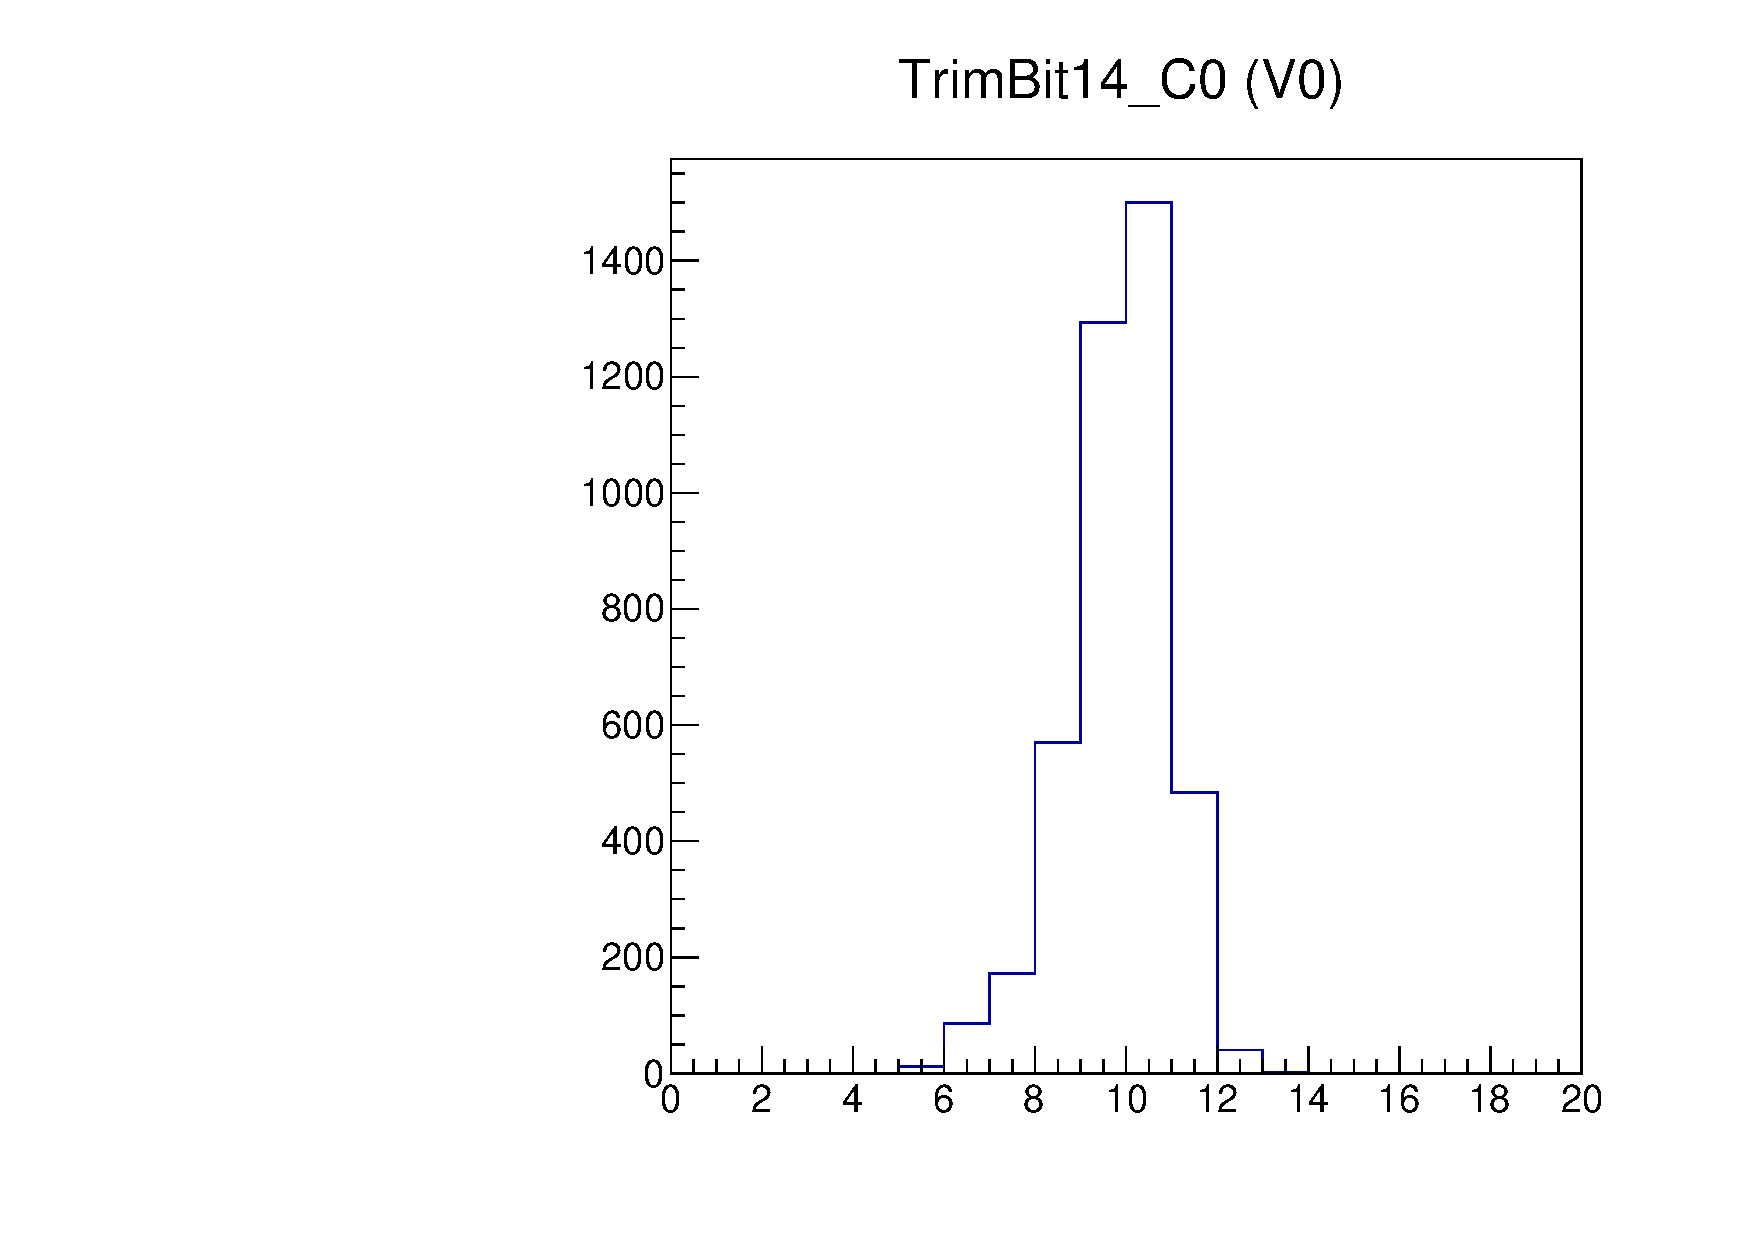
\includegraphics[width=1.0\textwidth]{figures/trim_TrimBit14.pdf}
  \caption{1D distribution of difference of Figure~\ref{fig:trim_thr_TrimBitsThr0_Vcal} and Figure~\ref{fig:trim_thr_TrimThr_trim14_Vcal}.
           Pixels with a faulty trim bit would populate the bin at zero.}
  \label{fig:trim_TrimBit14}
\end{minipage}
\end{figure}

\begin{figure}[!htp]
\centering
\begin{minipage}{0.45\textwidth}
  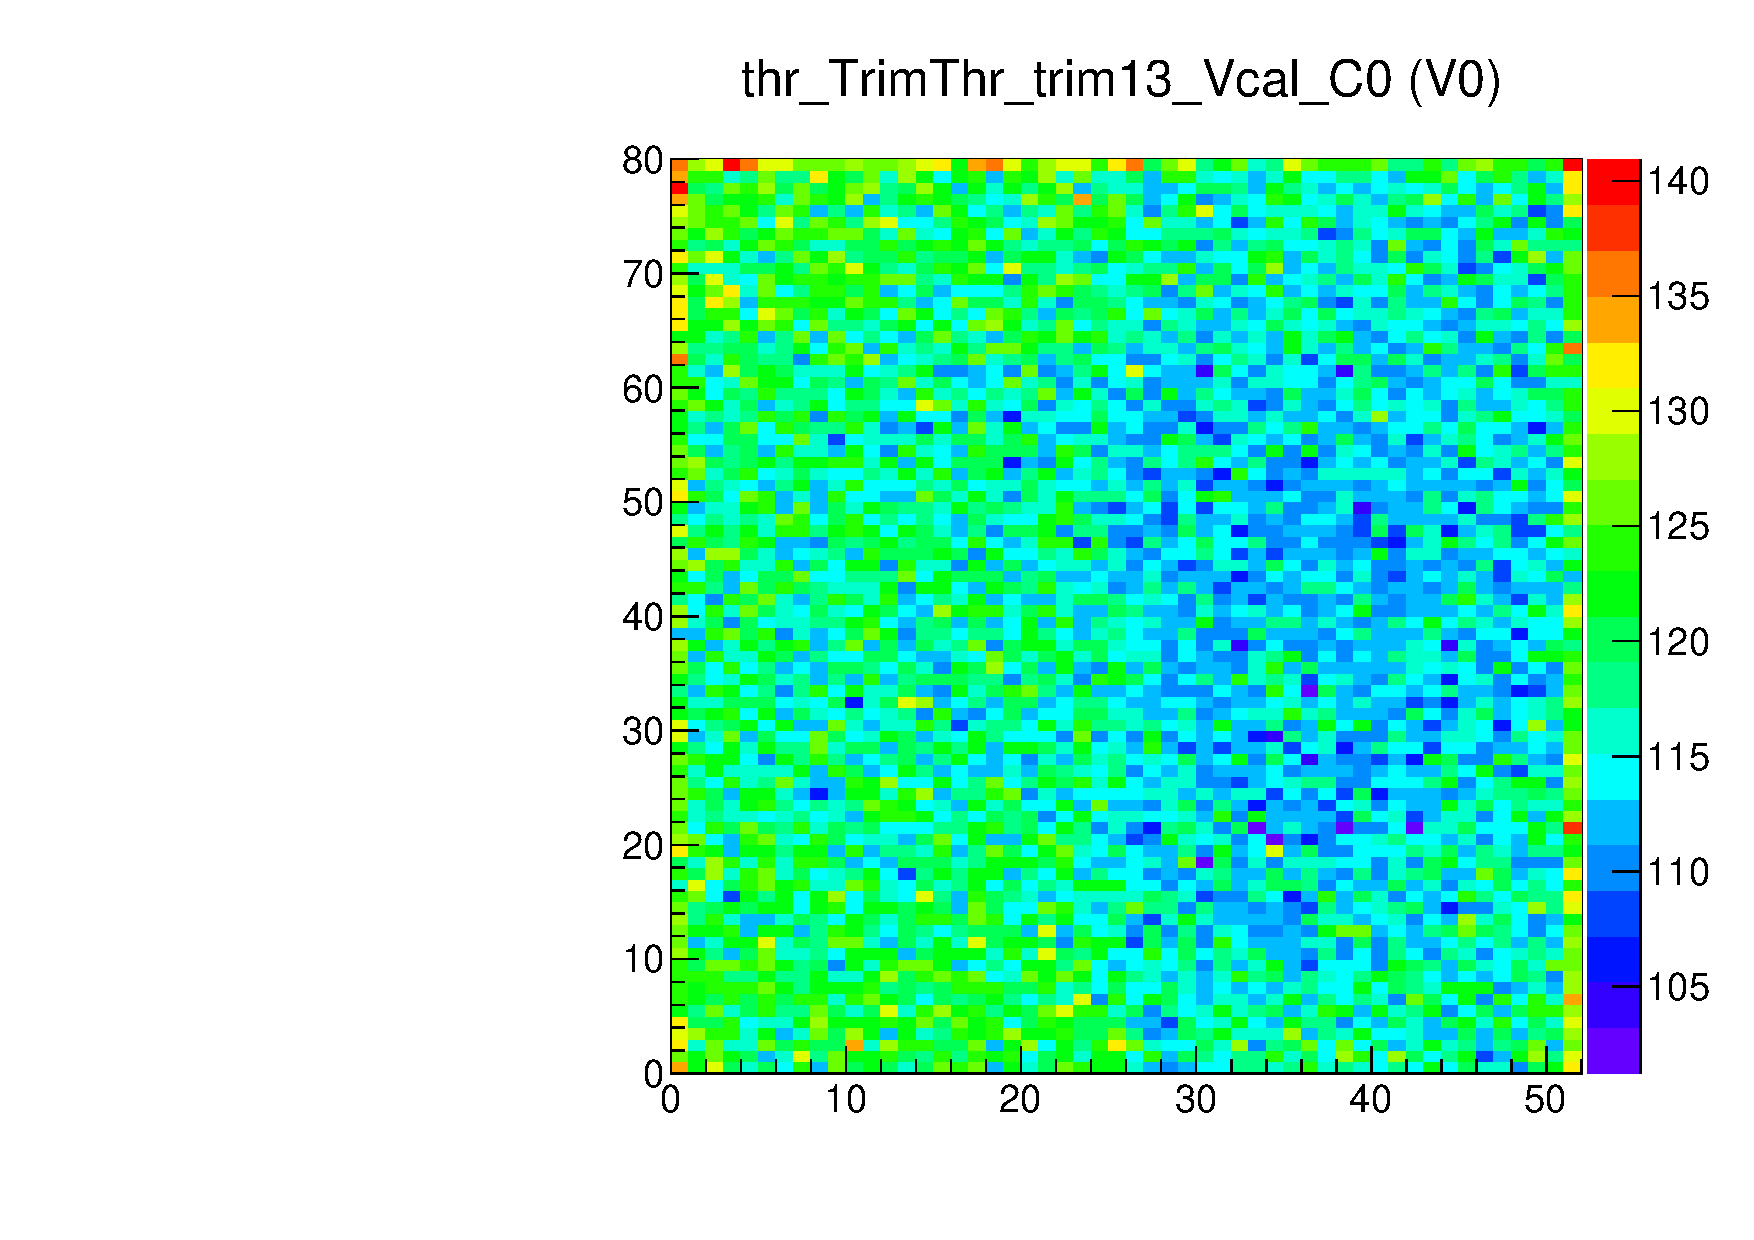
\includegraphics[width=1.0\textwidth]{figures/trim_thr_TrimThr_trim13_Vcal.pdf}
  \caption{\roc map of \vcal thresholds with \trimbits=13 [1101].}
  \label{fig:trim_thr_TrimThr_trim13_Vcal}
\end{minipage}
\hspace{0.3cm}
\begin{minipage}{0.45\textwidth}
  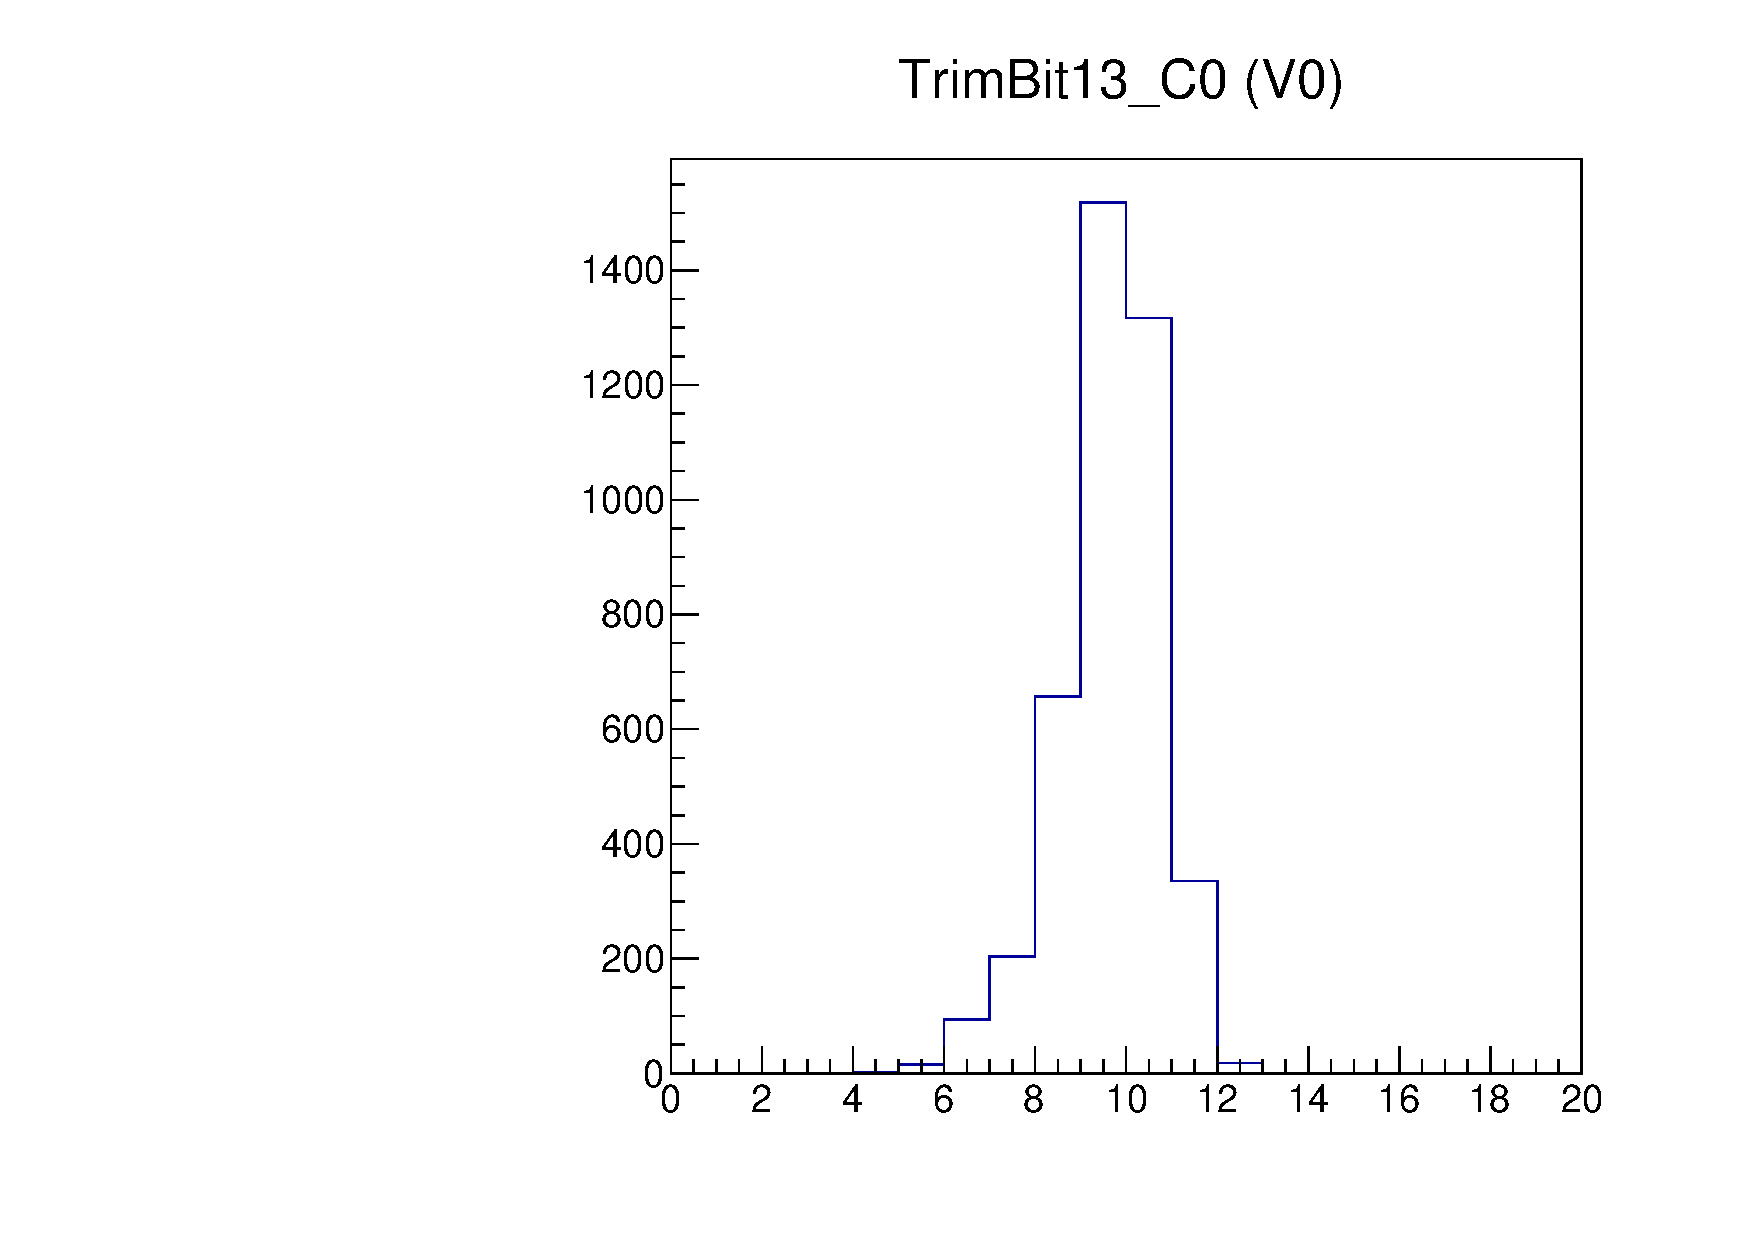
\includegraphics[width=1.0\textwidth]{figures/trim_TrimBit13.pdf}
  \caption{1D distribution of difference of Figure~\ref{fig:trim_thr_TrimBitsThr0_Vcal} and Figure~\ref{fig:trim_thr_TrimThr_trim13_Vcal}.
           Pixels with a faulty trim bit would populate the bin at zero.}
  \label{fig:trim_TrimBit13}
\end{minipage}
\end{figure}

\begin{figure}[!htp]
\centering
\begin{minipage}{0.45\textwidth}
  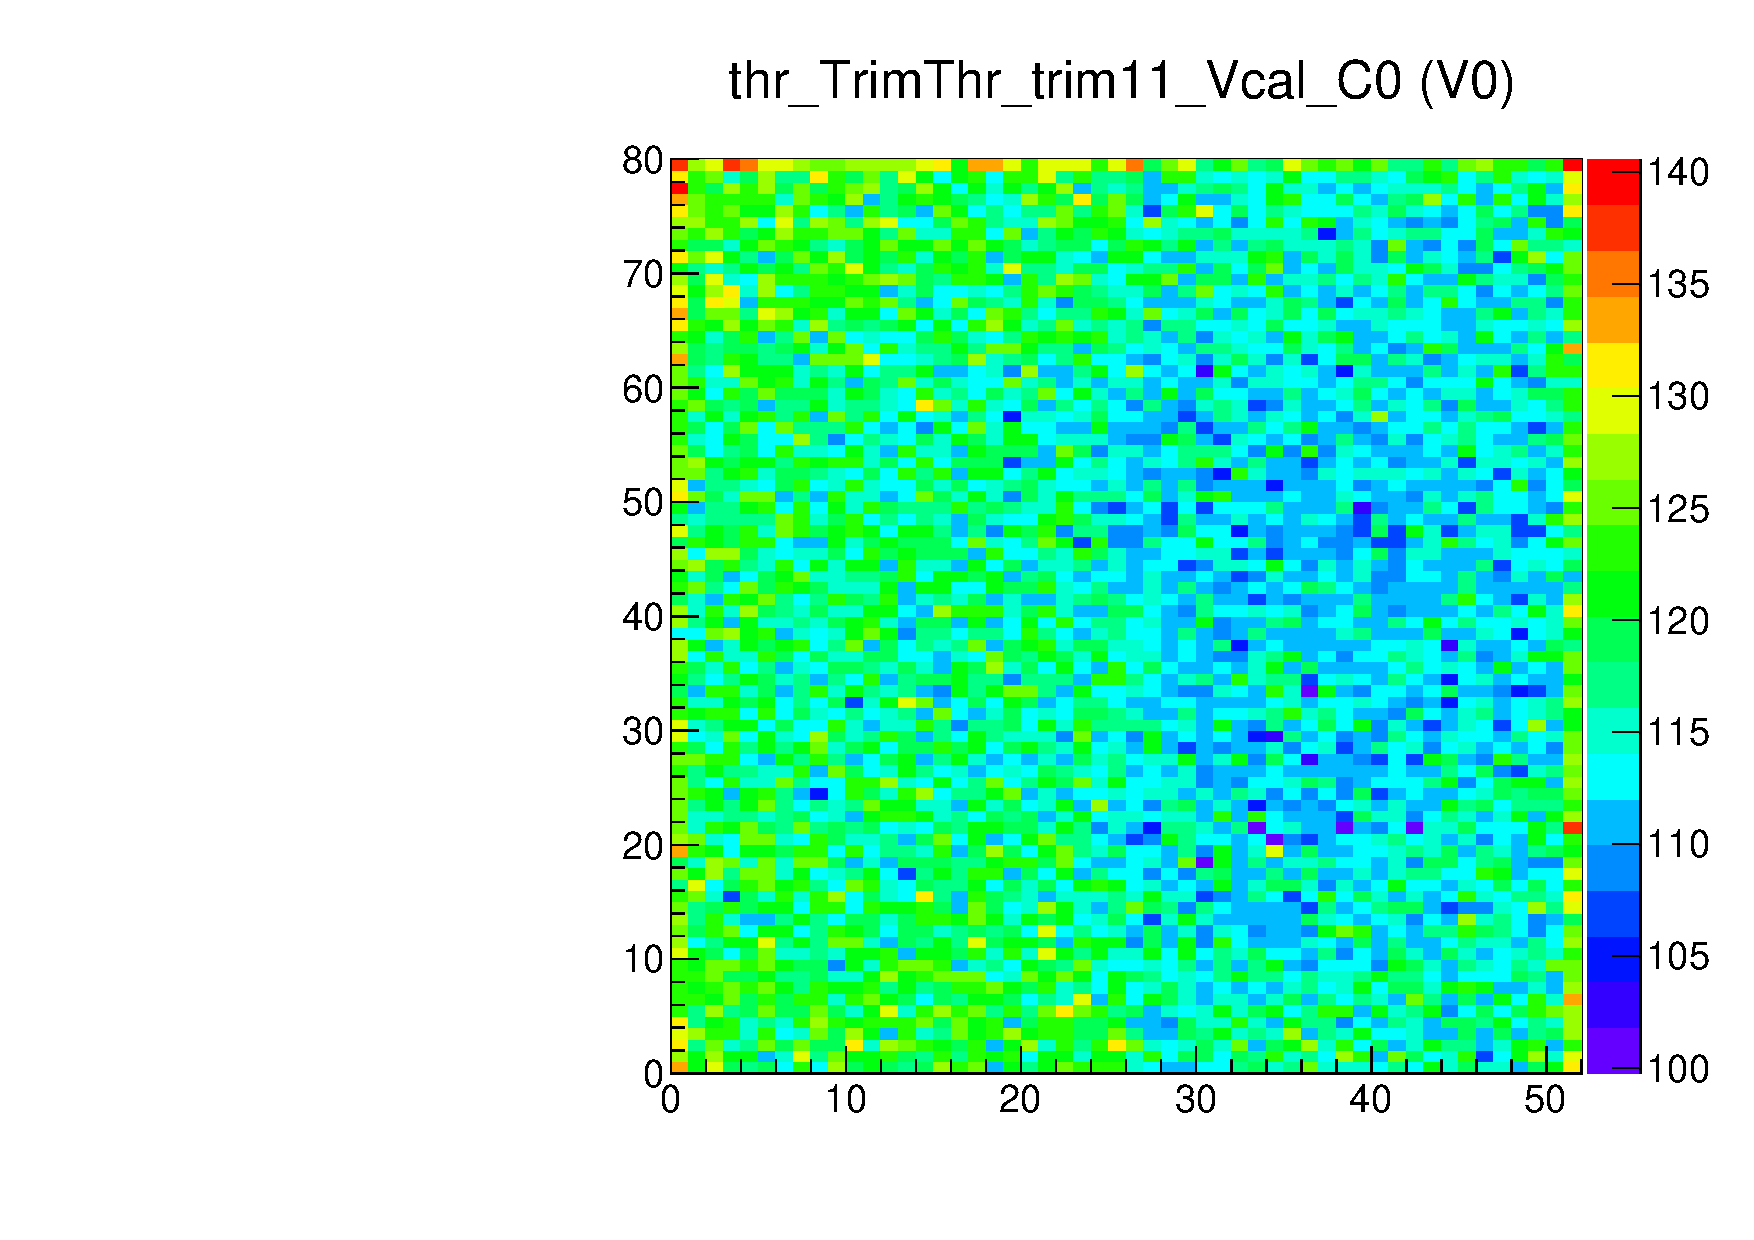
\includegraphics[width=1.0\textwidth]{figures/trim_thr_TrimThr_trim11_Vcal.pdf}
  \caption{\roc map of \vcal thresholds with \trimbits=11 [1011].}
  \label{fig:trim_thr_TrimThr_trim11_Vcal}
\end{minipage}
\hspace{0.3cm}
\begin{minipage}{0.45\textwidth}
  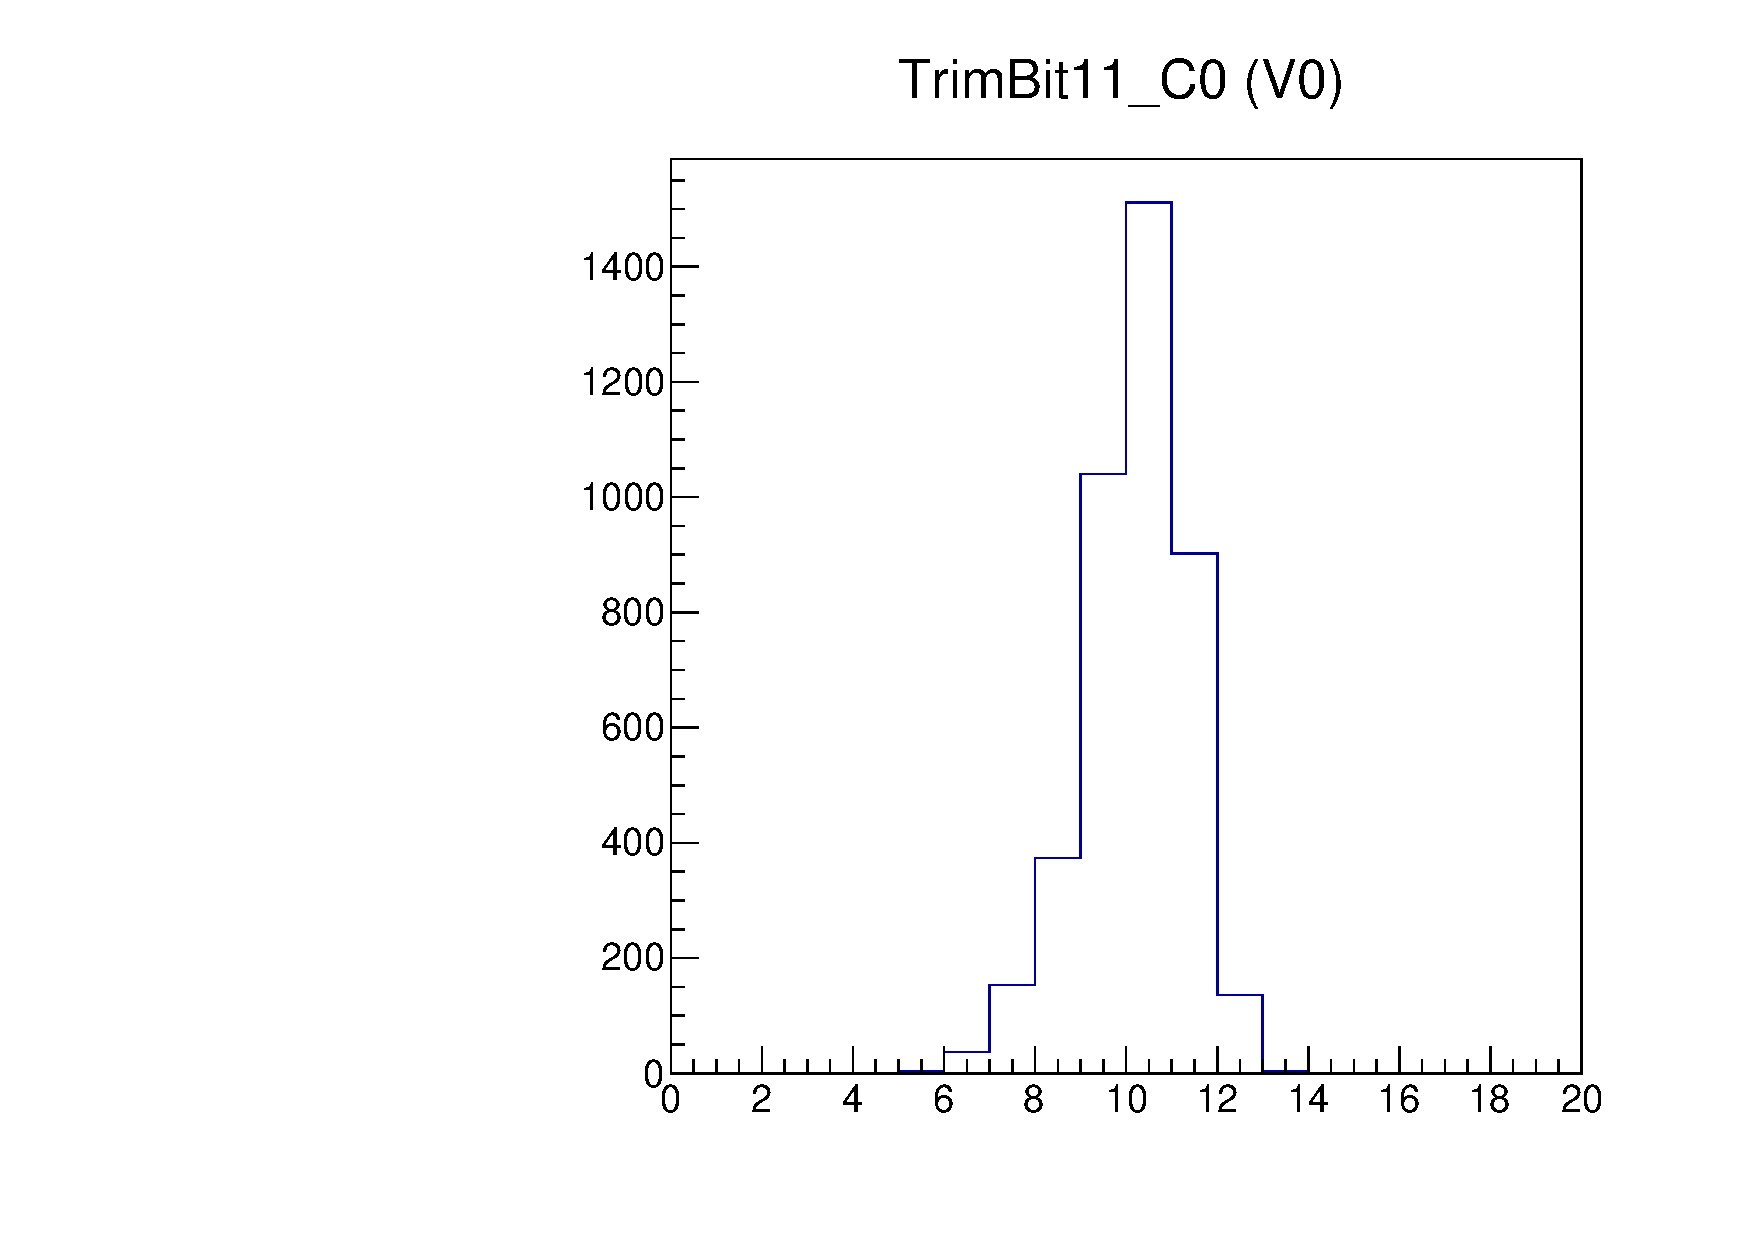
\includegraphics[width=1.0\textwidth]{figures/trim_TrimBit11.pdf}
  \caption{1D distribution of difference of Figure~\ref{fig:trim_thr_TrimBitsThr0_Vcal} and Figure~\ref{fig:trim_thr_TrimThr_trim11_Vcal}.
           Pixels with a faulty trim bit would populate the bin at zero.}
  \label{fig:trim_TrimBit11}
\end{minipage}
\end{figure}

\begin{figure}[!htp]
\centering
\begin{minipage}{0.45\textwidth}
  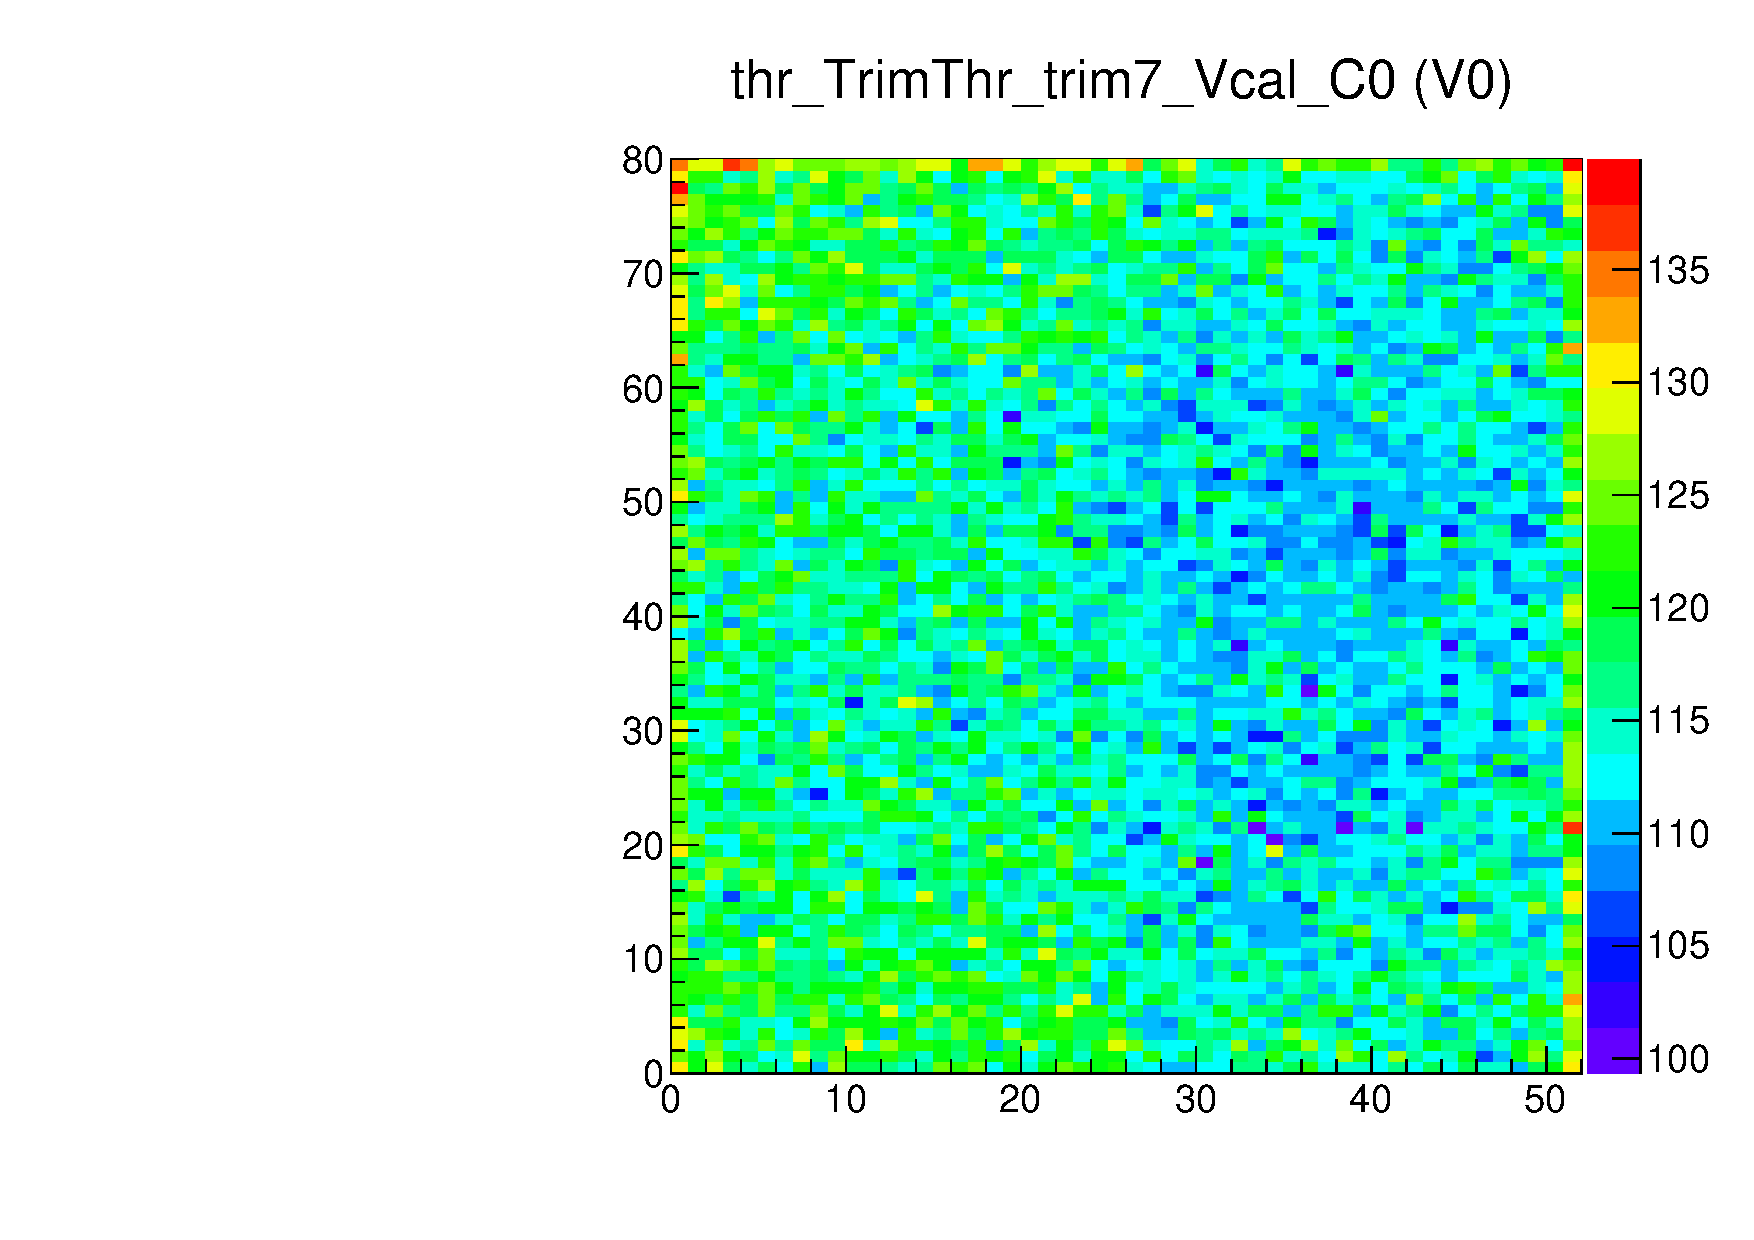
\includegraphics[width=1.0\textwidth]{figures/trim_thr_TrimThr_trim7_Vcal.pdf}
  \caption{\roc map of \vcal thresholds with \trimbits=7 [0111].}
  \label{fig:trim_thr_TrimThr_trim7_Vcal}
\end{minipage}
\hspace{0.3cm}
\begin{minipage}{0.45\textwidth}
  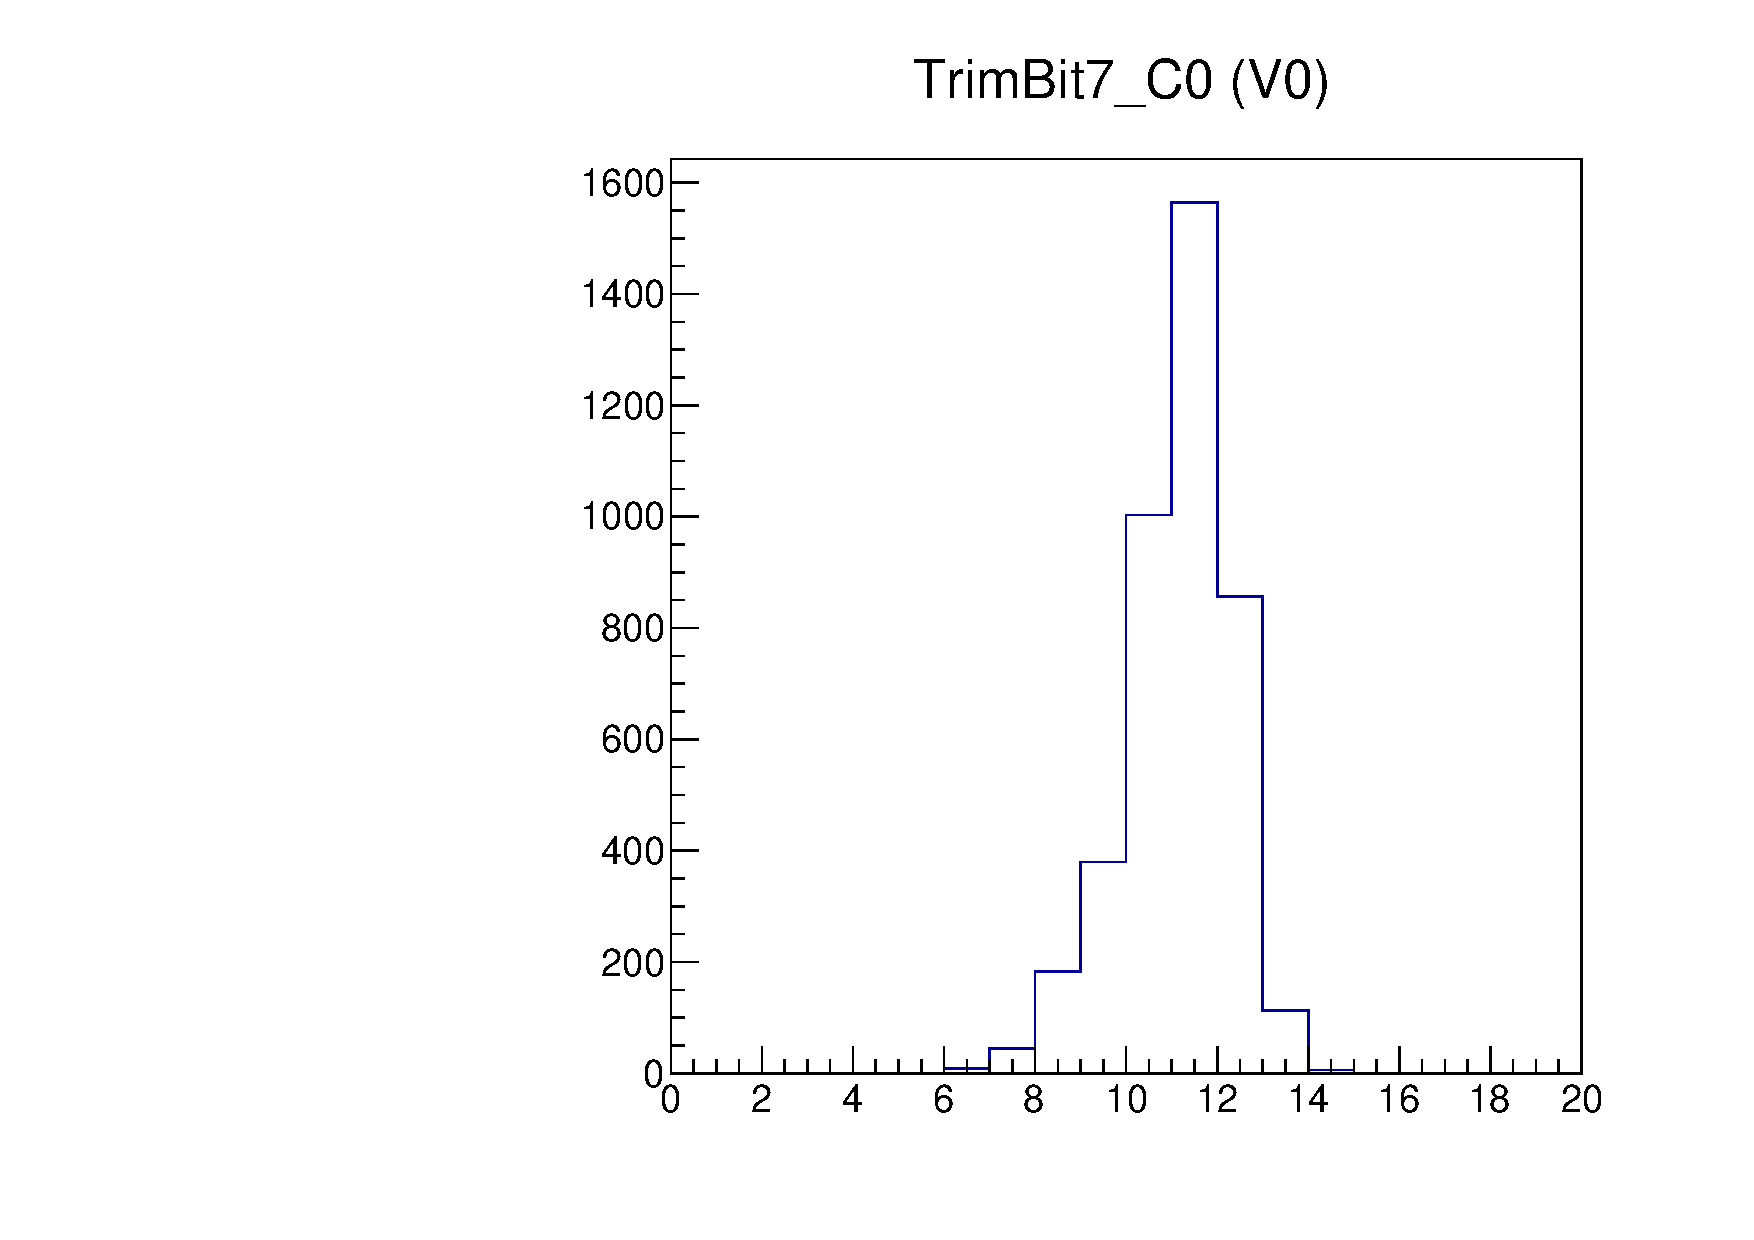
\includegraphics[width=1.0\textwidth]{figures/trim_TrimBit7.pdf}
  \caption{1D distribution of difference of Figure~\ref{fig:trim_thr_TrimBitsThr0_Vcal} and Figure~\ref{fig:trim_thr_TrimThr_trim7_Vcal}.
           Pixels with a faulty trim bit would populate the bin at zero.}
  \label{fig:trim_TrimBit7}
\end{minipage}
\end{figure}



% ----------------------------------------------------------------------

\newpage

\subsection{\phopt Test}
\label{ss:phoptimization}

\subsubsection{Purpose}

The \phopt test is responsible for setting an appropriate dynamic range for the 8-bit ADC that digitizes the recorded pulse height.
The ADC is located in the Controller and Interface Block of the \roc.
It can be seen in the bottom right box of Figure~\ref{fig:puc}.
The two \dacs used to configure the ADC are \phoffset and \phscale.
\phoffset adds a constant offset to the pulse height measurement,
while \phscale effectively sets the gain of the ADC.
The \phopt test is designed to optimize these \dacs based on a highly sensitive and highly insensitive pixel in the given \roc, 
or, in other words, pixels with a very high and very low inherent gain.
To use the ADC most effectively, the range of the ADC PH response as a function of \vcal needs to be optimized.
On the low end, the ADC should provide a PH well above noise for the low-gain pixel near the lowest \vcal that registers a hit on it.
On the high end, the ADC should saturate for the high-gain pixel at some user-defined \vcal well below the maximum \vcal the \roc can provide.
This allows the signal strength required for saturation to be measured and recorded for all pixels.
These two conditions are translated into two constraints used to simultaneously find a solution for the values of \phoffset and \phscale.
The constraints applied are 1: the low-gain pixel should have a reasonably large PH (default is 20) at its \vcal turn-on threshold,
and 2: the high-gain pixel should saturate (PH reaches 255) at a user-defined signal strength (default is \vcal = 100 (high range)).

\subsubsection{Methodology}

The \phopt test proceeds in two steps:  
First, it identifies a low-gain and high-gain pixel for use in optimizing \phscale and \phoffset.
In this process, care is taken not to choose anomalous pixels.
Secondly, it maps the pulse height responses of these two pixels as a function of \phscale and \phoffset.
The maps for these two pixels are then combined to find the optimal values for \phscale and \phoffset.
After the optimal values for \phscale and \phoffset are set, several validation plots are made and recorded in the output file.
\\\\
First, the test identifies a low-gain and high-gain pixels using the same methodology for each.
Pixels within 3 columns or 5 rows of the edge of the \roc are not considered, 
unless a suitable pixel cannot be found using those fiducial cuts, in which case those requirements are relaxed.
In each case, the PH for each pixel is obtained at a chosen \vcal (Figures~\ref{fig:phopt_minphmap},~\ref{fig:phopt_maxphmap}), 
and a 1D distribution of all PHs is created for each \roc (Figures~\ref{fig:phopt_dist_minphmap},~\ref{fig:phopt_dist_maxphmap}). 
From this distribution, a pixel is chosen that is separated from the edge of the distribution by a chosen percentile of safety margin.
This helps avoid choosing an anomalous pixel.
For finding the high-gain pixel, this process is performed with the maximum calibration pulse strength, \vcal=255 (high range).
The safety margin is configurable, and by default is 98\%, i.e. a pixel will be chosen such that 98\% of pixels in the \roc have lower PHs.
For finding the low-gain pixel, the process is performed with a \vcal slightly higher than the \vcal trimming target, 
hard-coded to \vcal=60 (low range).
For the chosen low-gain pixel, the \vcal value is found at which the pixel starts firing, 
defined as the point in the PH vs. \vcal curve at which PH=10.
This minimum \vcal value is recorded for use in the following step of the test.
\\\\
Once the two pixels of interest have been identified, the test proceeds to the optimization of \phscale and \phoffset.
A 2D scan is performed over \phscale and \phoffset, returning the PH at each point in the 2D parameter space
(Figures~\ref{fig:phopt_minphvsdacdac_th2},~\ref{fig:phopt_maxphvsdacdac_th2}).
For the low-gain pixel, the scan is performed at the minimum \vcal found in the previous step.
For the high-gain pixel, the scan is performed at the user-defined ADC saturation target (default is \vcal = 100 (high range)).
The optimal regime for the low-gain pixel is when the pulse height value is near to some small safety margin (default 20) above zero.
The optimal regime for the high-gain pixel is when the ADC saturates at this \vcal, meaning that PH is near 255.
Each of these regimes defines a band in the \phoffset vs. \phscale plane.
The final values of \phscale and \phoffset are chosen from the intersection of these two bands (Figure~\ref{fig:phopt_solphvsdacdac_th2}).
\\\\
With the optimal values of \phscale and \phoffset set, several validation scans are performed.
First, PH vs. \vcal curves are produced for the chosen low-gain and high-gain pixels
(Figures~\ref{fig:phopt_PH_c5_r68},~\ref{fig:phopt_PH_c3_r15}).
Additionally, PH maps are produced at three \vcal values,
one low (defined as 10 DAC units above the minimum effective \vcal for the low-gain pixel)
(Figures~\ref{fig:phopt_PH_mapLowVcal},~\ref{fig:phopt_dist_PH_mapLowVcal}),
one medium (\vcal=50 (low range))
(Figures~\ref{fig:phopt_PH_mapVcal50},~\ref{fig:phopt_dist_PH_mapVcal50}),
and one high (chosen ADC saturation target)
(Figures~\ref{fig:phopt_PH_mapHiVcal},~\ref{fig:phopt_dist_PH_mapHiVcal}).

\subsubsection{Output}

% finding highest/lowest gain pixels

\begin{figure}[!htp]
\centering
\begin{minipage}{0.45\textwidth}
  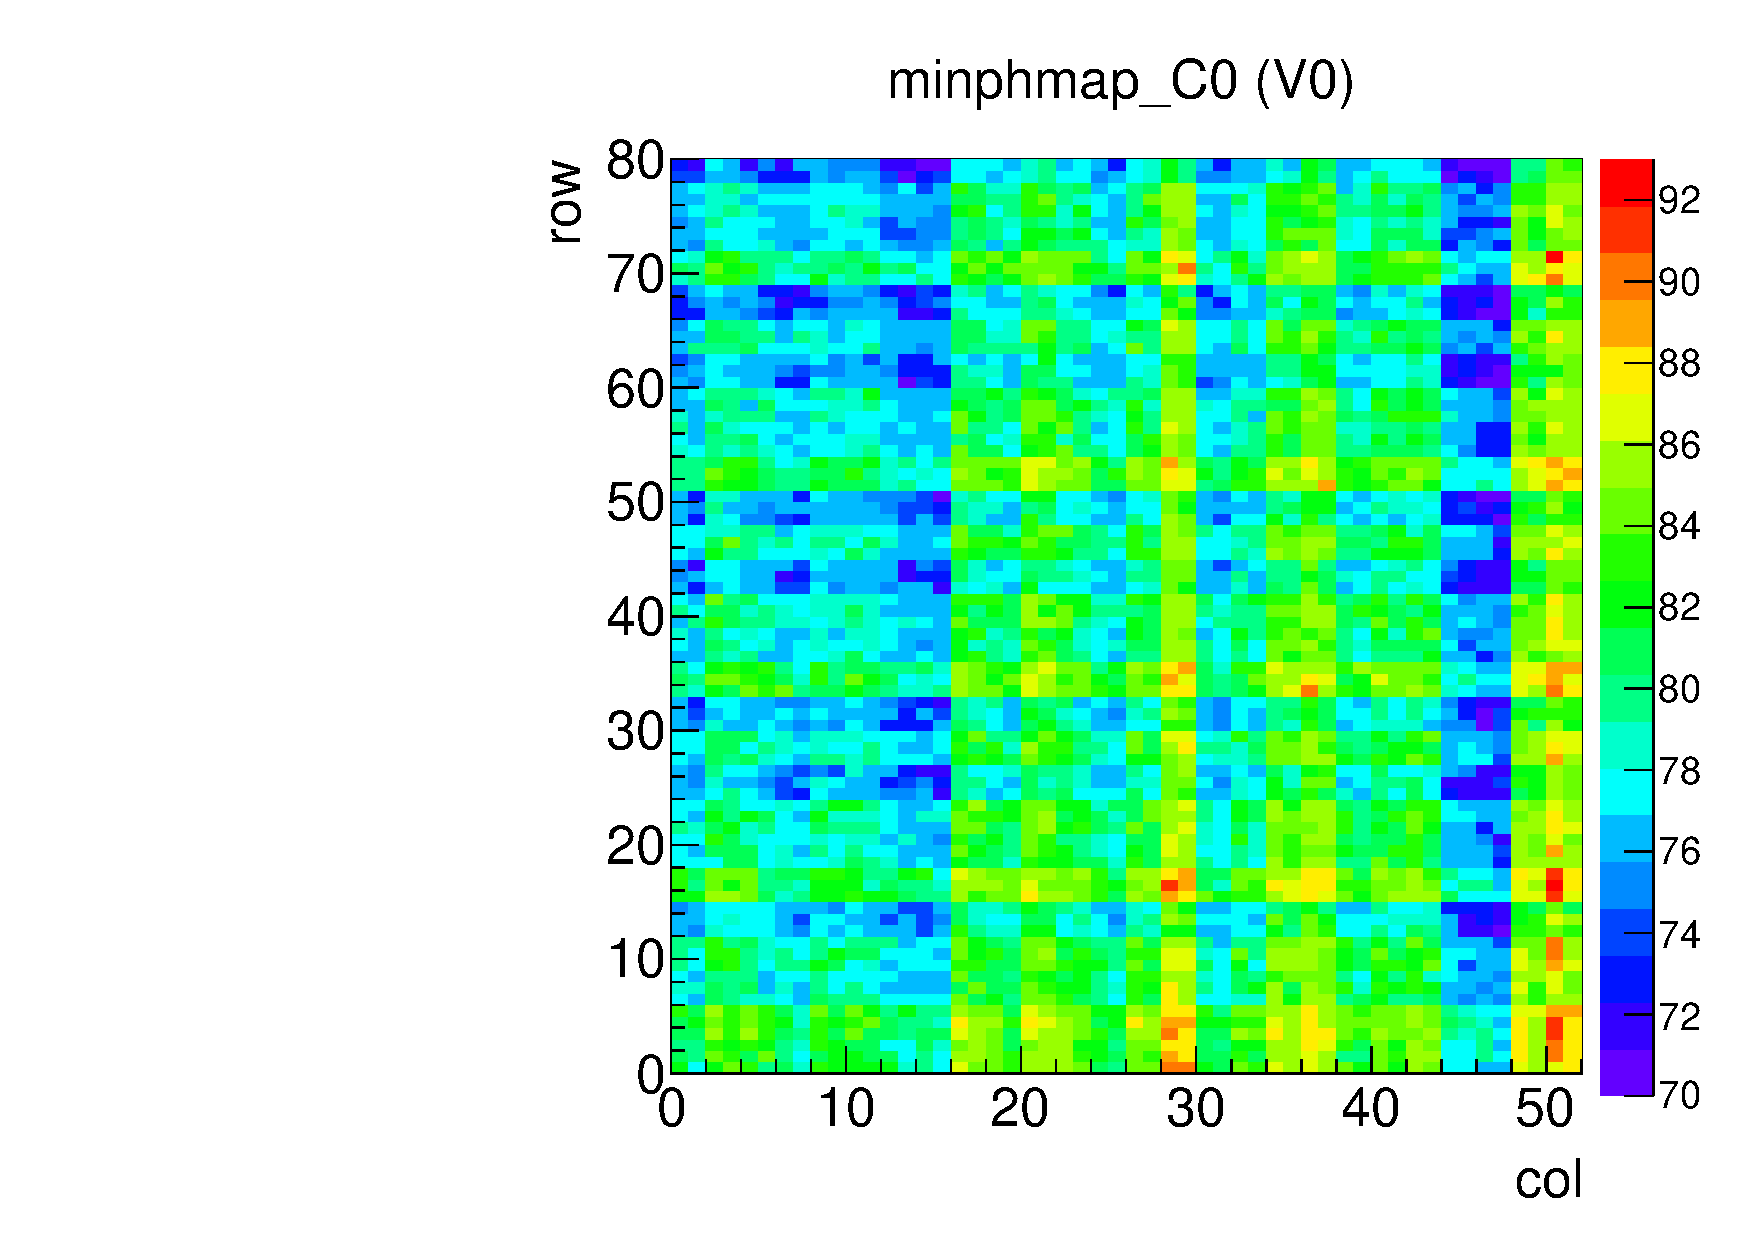
\includegraphics[width=1.0\textwidth]{figures/phopt_minphmap.pdf}
  \caption{\roc map of pulse heights with \vcal=60 (low range).}
  \label{fig:phopt_minphmap}
\end{minipage}
\hspace{0.3cm}
\begin{minipage}{0.45\textwidth}
  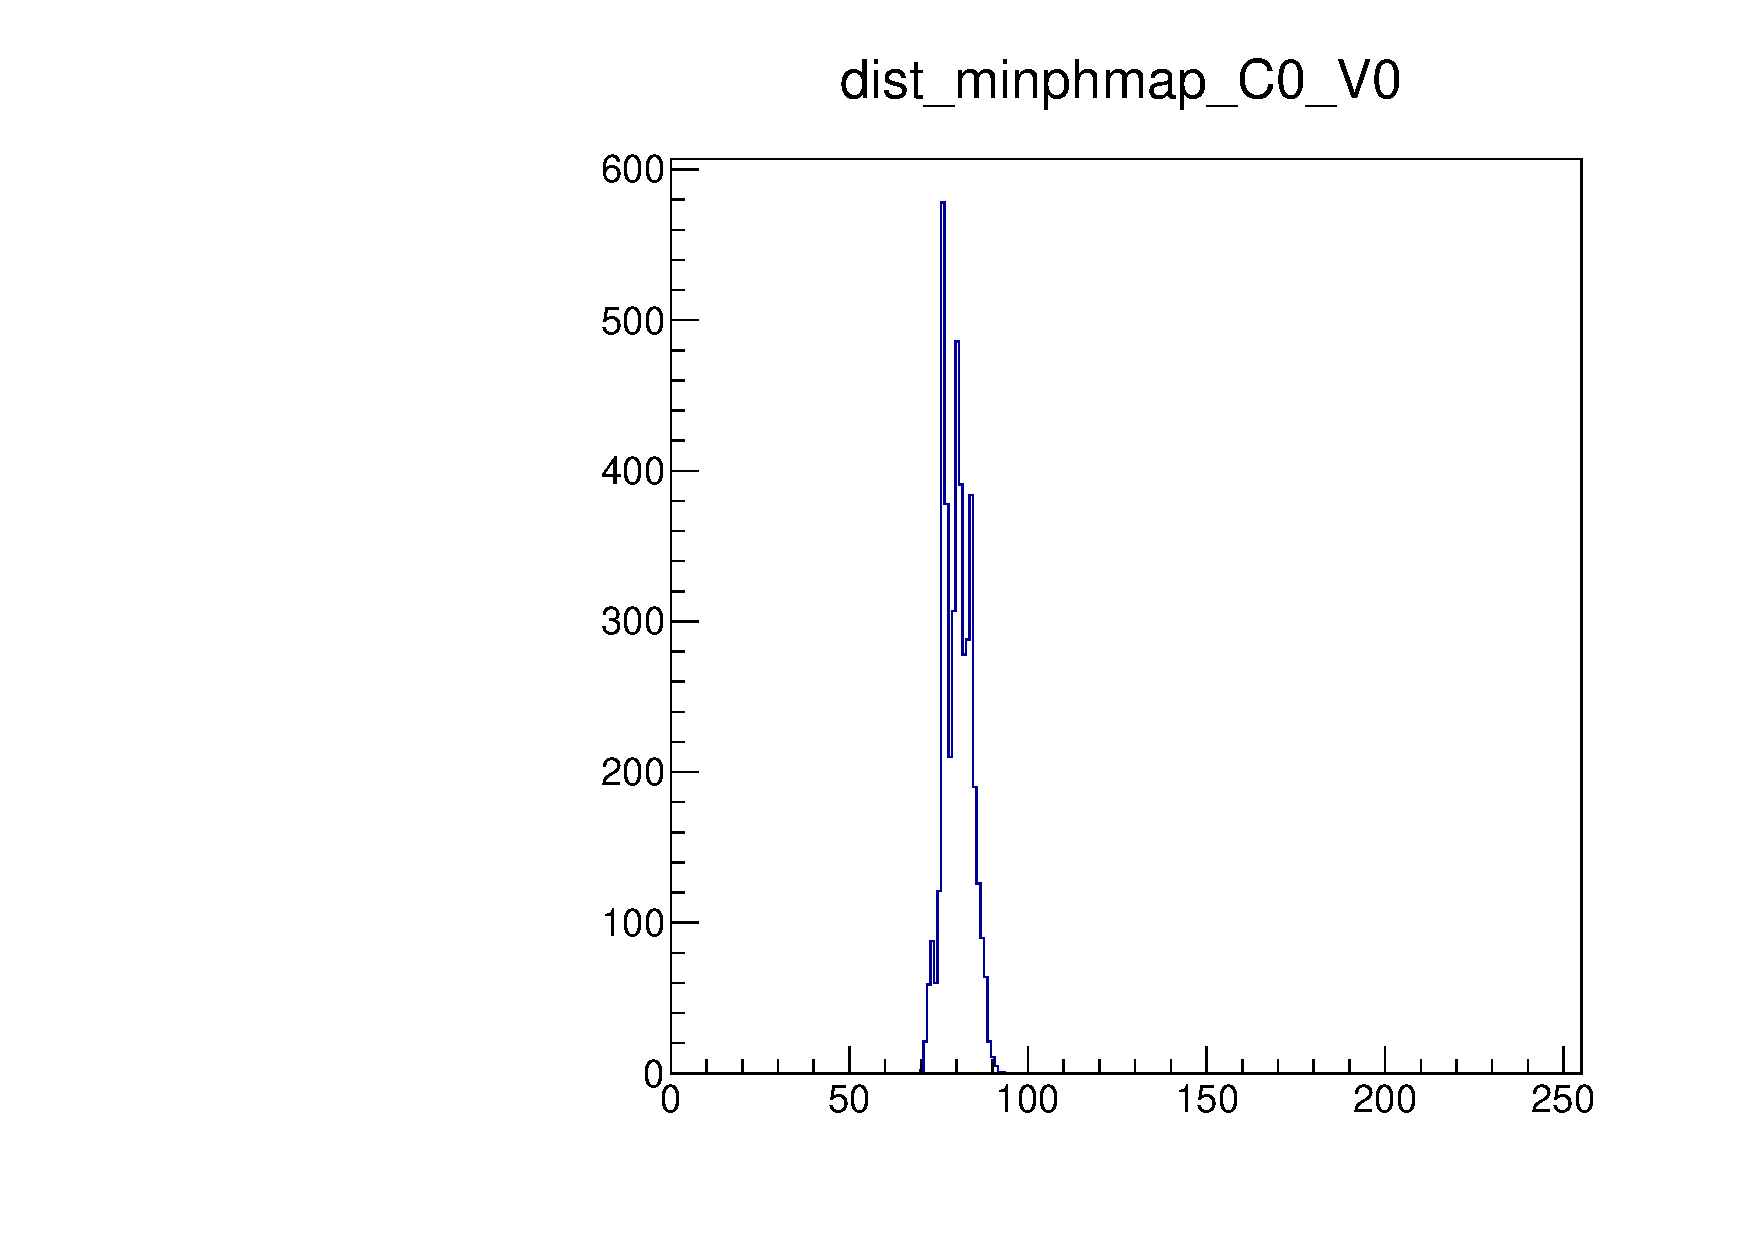
\includegraphics[width=1.0\textwidth]{figures/phopt_dist_minphmap.pdf}
  \caption{1D distribution of Figure~\ref{fig:phopt_minphmap}
           used to identify low-gain pixel.}
  \label{fig:phopt_dist_minphmap}
\end{minipage}
\end{figure}

\begin{figure}[!htp]
\centering
\begin{minipage}{0.45\textwidth}
  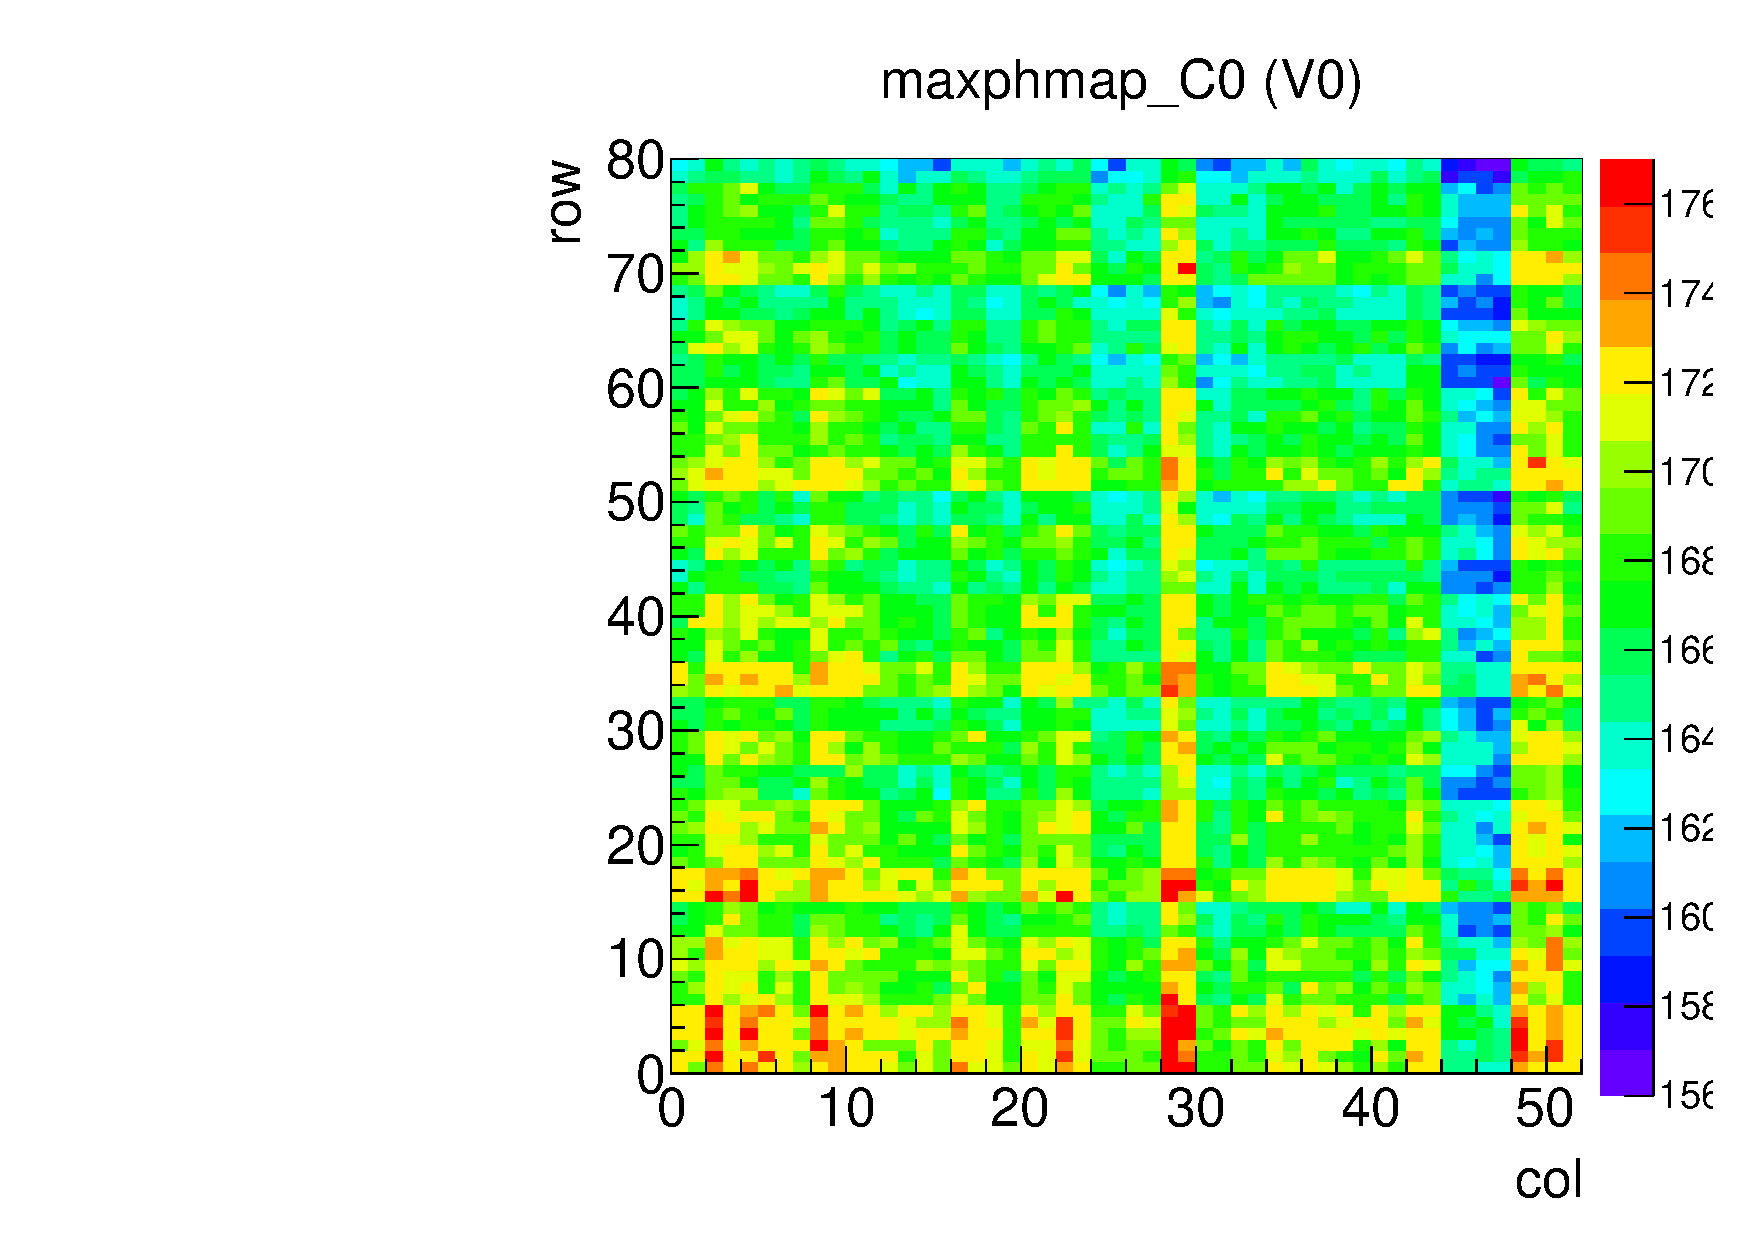
\includegraphics[width=1.0\textwidth]{figures/phopt_maxphmap.pdf}
  \caption{\roc map of pulse heights with \vcal=255 (high range).}
  \label{fig:phopt_maxphmap}
\end{minipage}
\hspace{0.3cm}
\begin{minipage}{0.45\textwidth}
  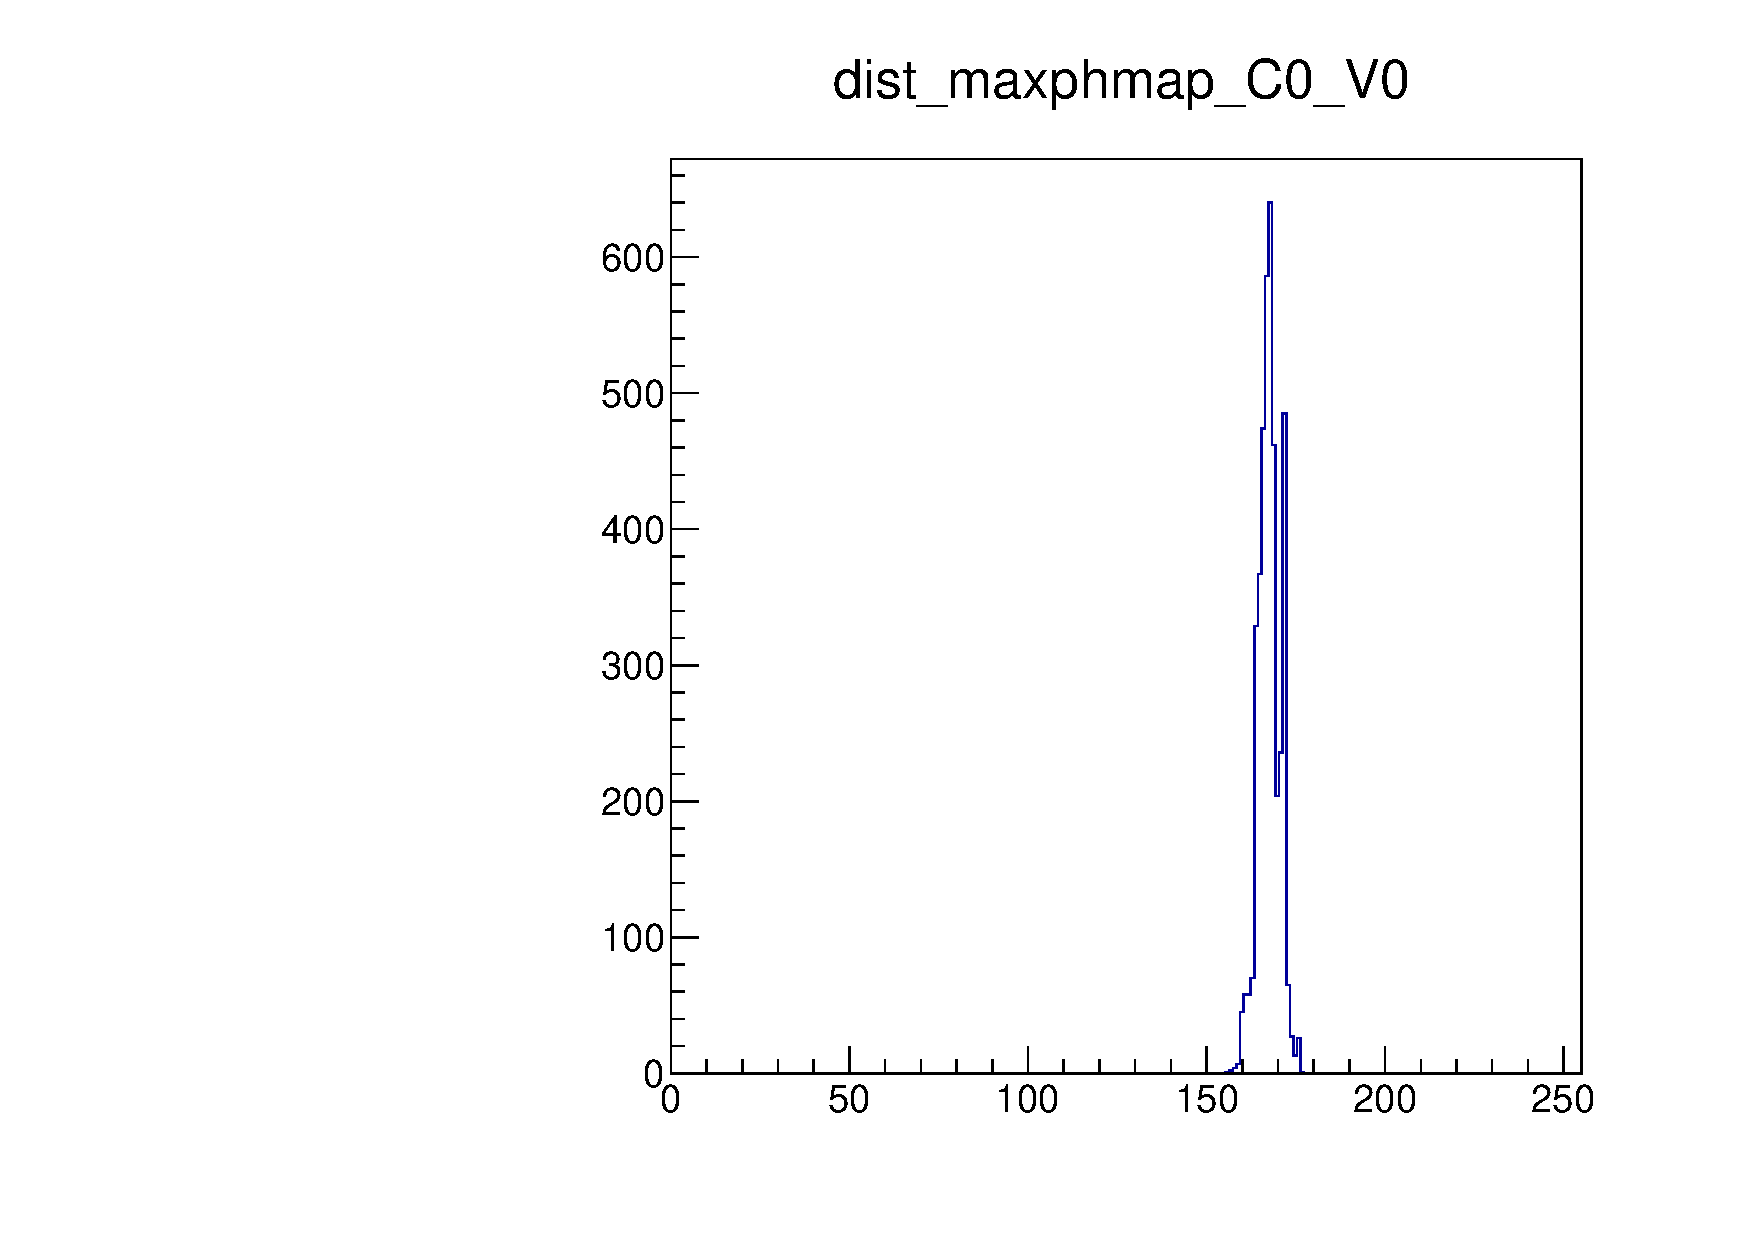
\includegraphics[width=1.0\textwidth]{figures/phopt_dist_maxphmap.pdf}
  \caption{1D distribution of Figure~\ref{fig:phopt_maxphmap}
           used to identify high-gain pixel.}
  \label{fig:phopt_dist_maxphmap}
\end{minipage}
\end{figure}

% getting maps for optimization

\begin{figure}[!htp]
\centering
\begin{minipage}{0.45\textwidth}
  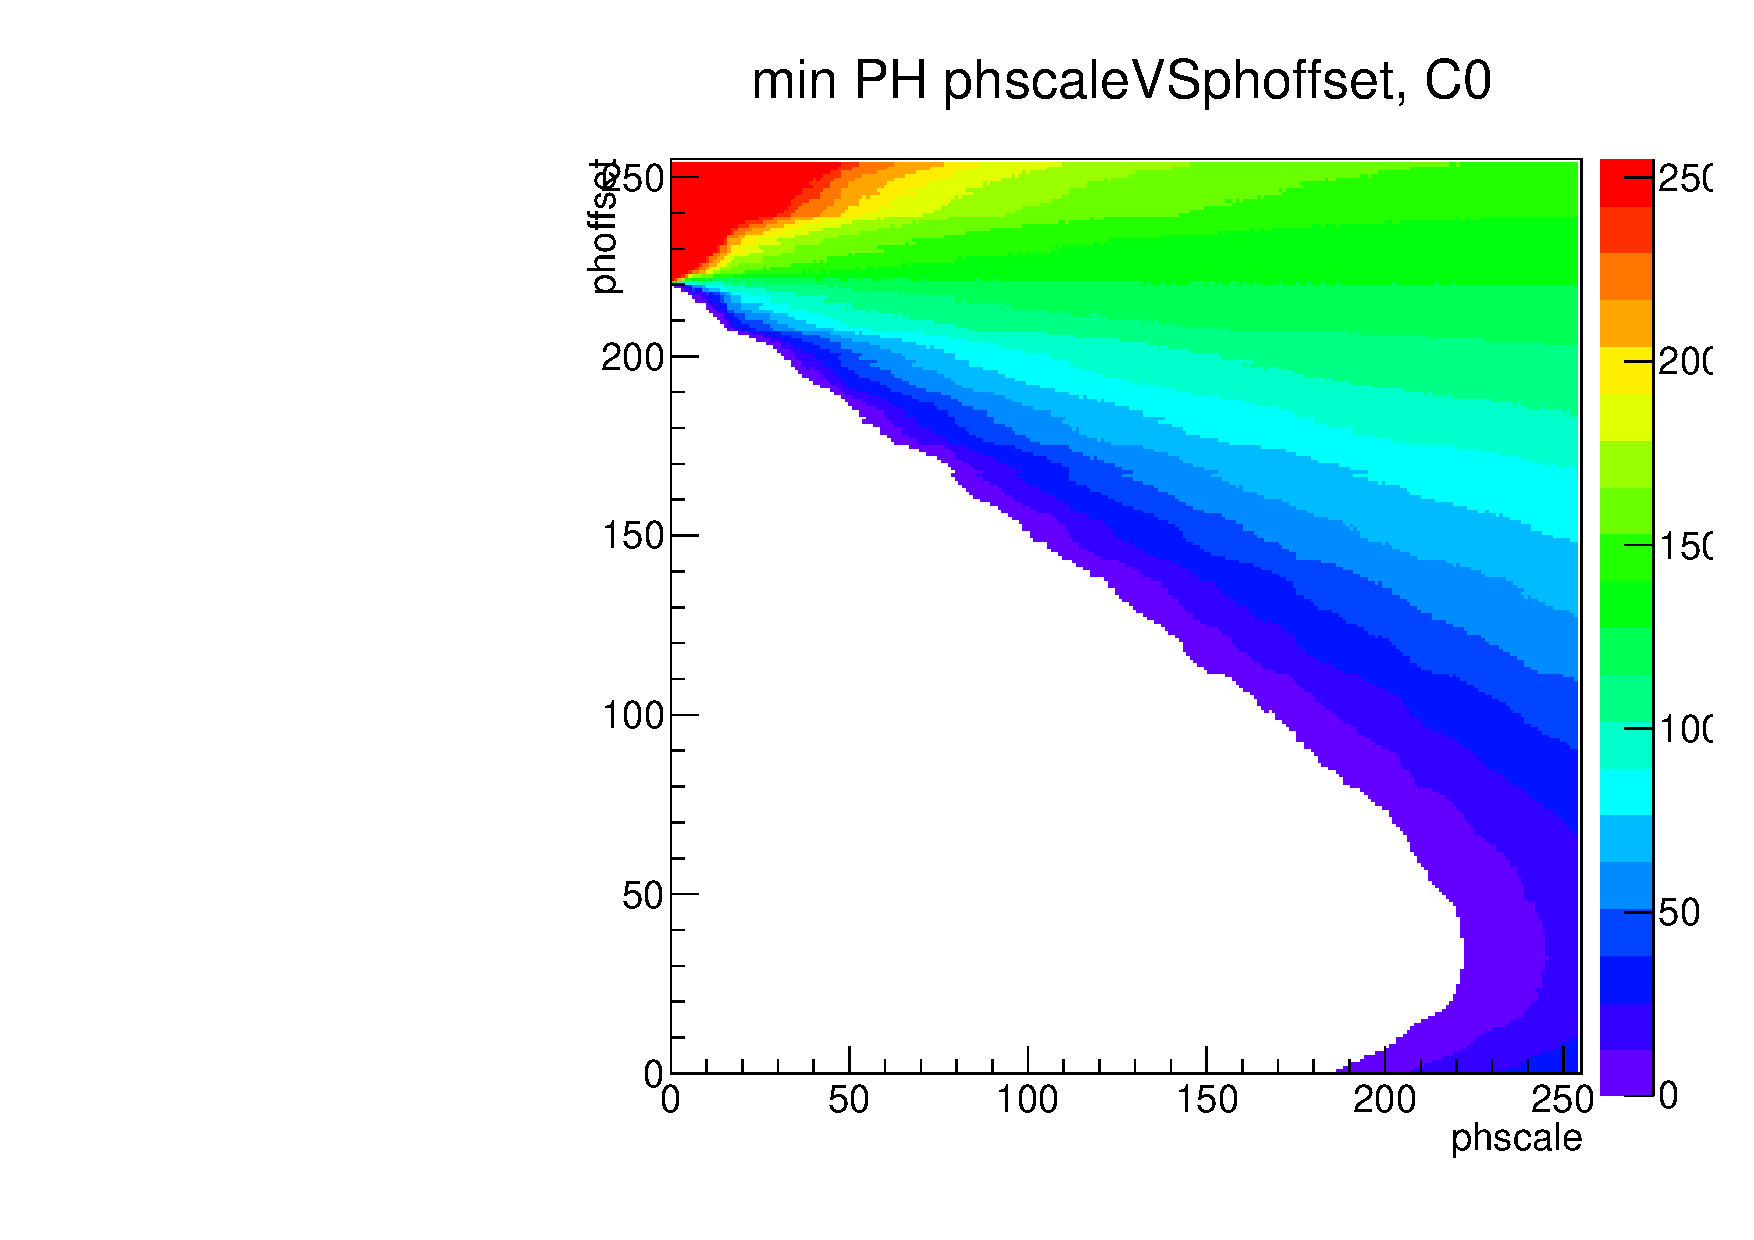
\includegraphics[width=1.0\textwidth]{figures/phopt_minphvsdacdac_th2.pdf}
  \caption{Measured PH in the \phoffset vs. \phscale plane for previously identified low-gain pixel
           with minimum \vcal required to fire the pixel.}
  \label{fig:phopt_minphvsdacdac_th2}
\end{minipage}
\hspace{0.3cm}
\begin{minipage}{0.45\textwidth}
  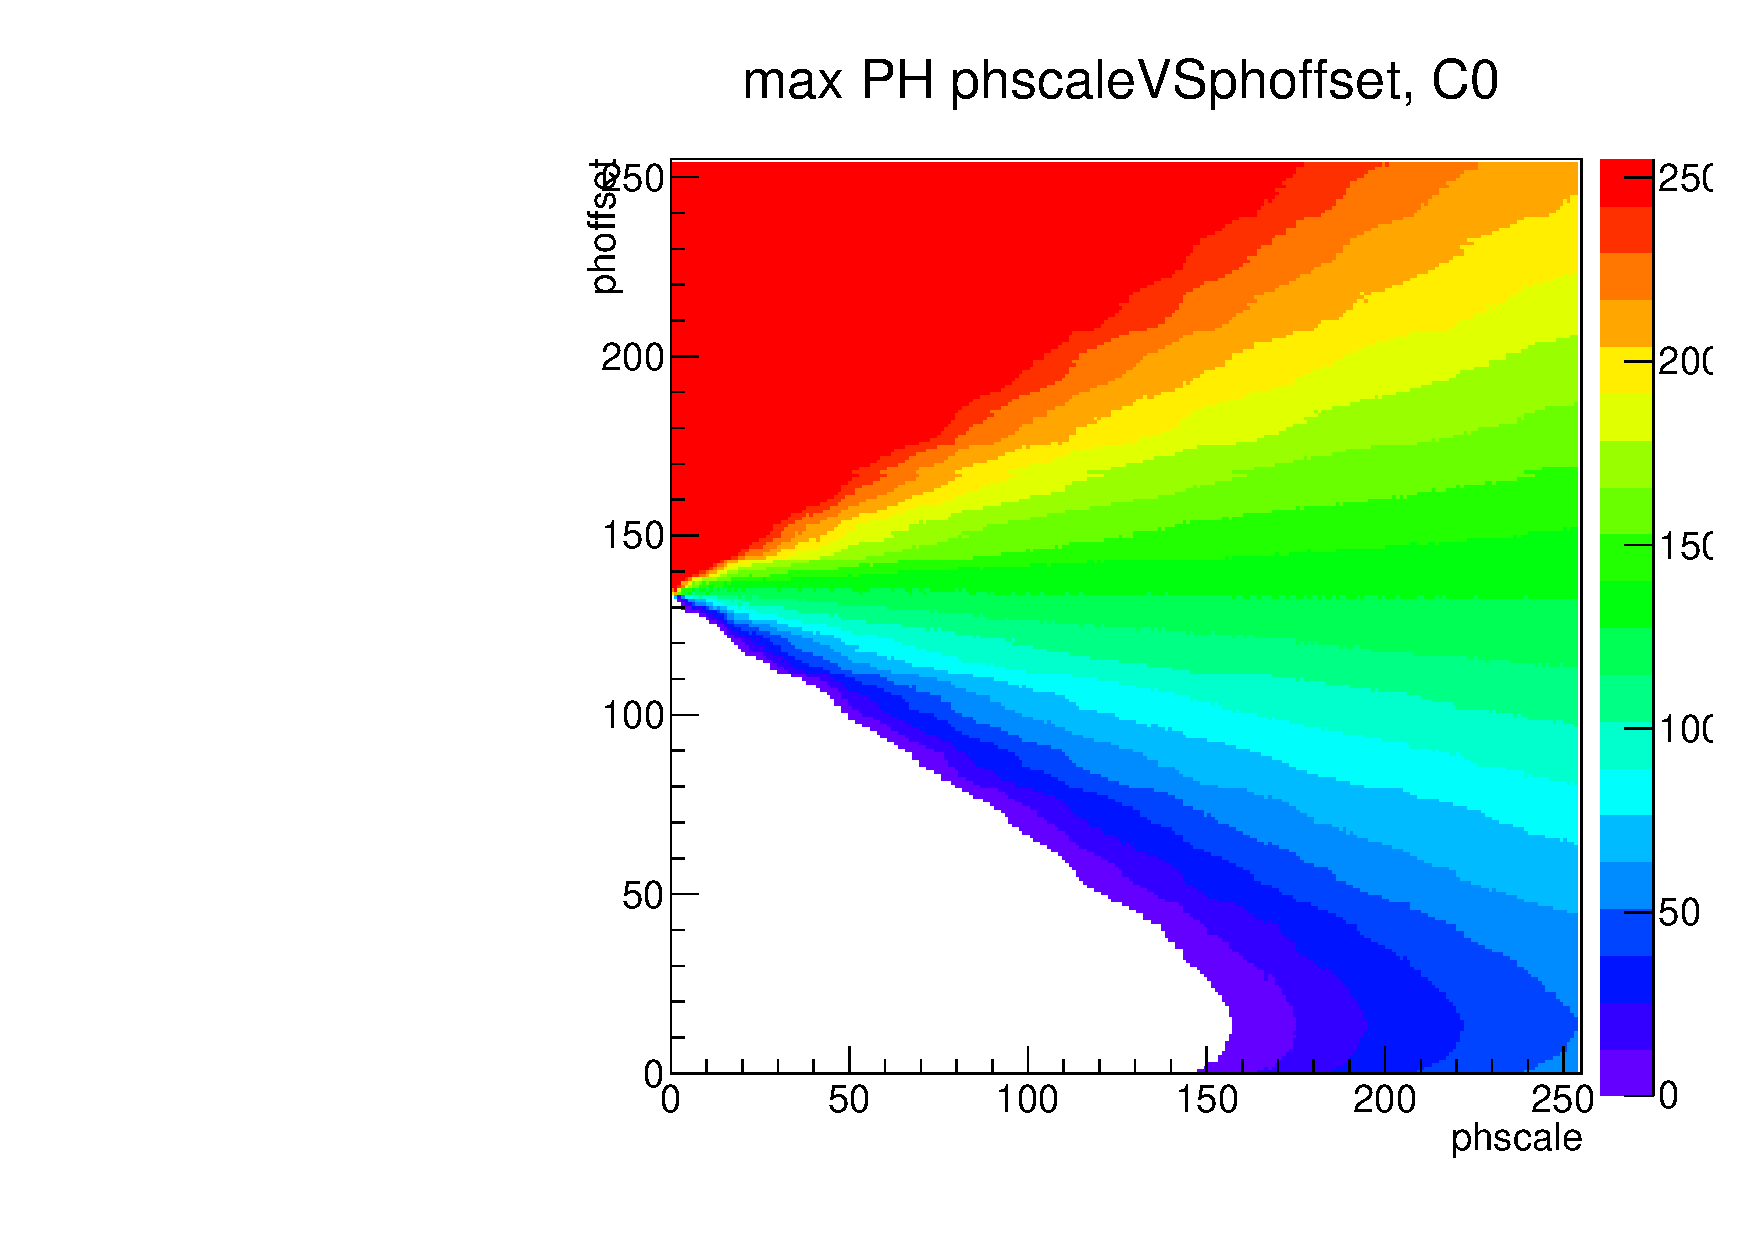
\includegraphics[width=1.0\textwidth]{figures/phopt_maxphvsdacdac_th2.pdf}
  \caption{Measured PH in the \phoffset vs. \phscale plane for previously identified high-gain pixel
           with \vcal set to the chosen ADC saturation point.}
  \label{fig:phopt_maxphvsdacdac_th2}
\end{minipage}
\end{figure}

\begin{figure}[!htp]
\centering
\begin{minipage}{0.45\textwidth}
  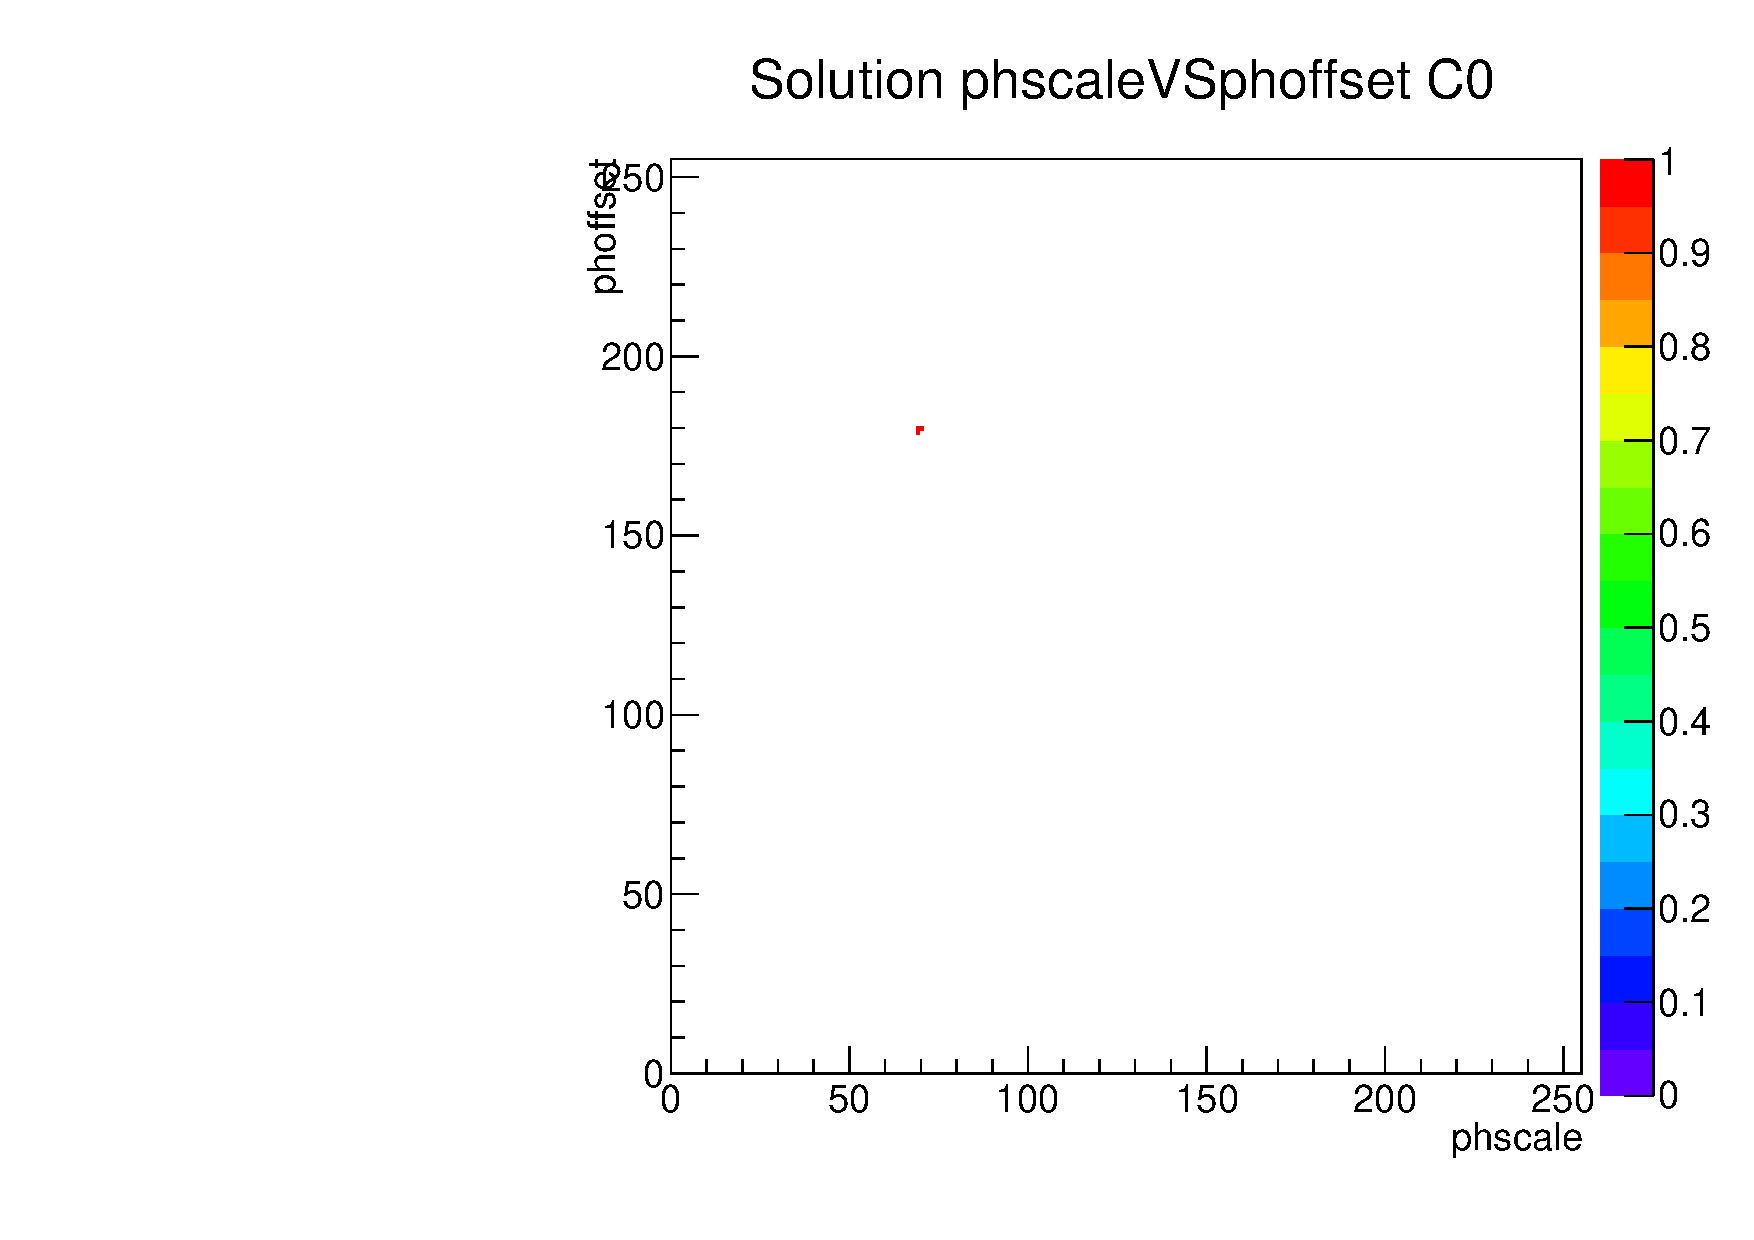
\includegraphics[width=1.0\textwidth]{figures/phopt_solphvsdacdac_th2.pdf}
  \caption{Overlap of optimal regimes in Figures~\ref{fig:phopt_minphvsdacdac_th2} and~\ref{fig:phopt_maxphvsdacdac_th2}.
           A red entry signifies an optimal pair of \phoffset and \phscale values.}
  \label{fig:phopt_solphvsdacdac_th2}
\end{minipage}
\end{figure}

% gain plots for highest/lowest gain pixels with optimized DACs

\begin{figure}[!htp]
\centering
\begin{minipage}{0.45\textwidth}
  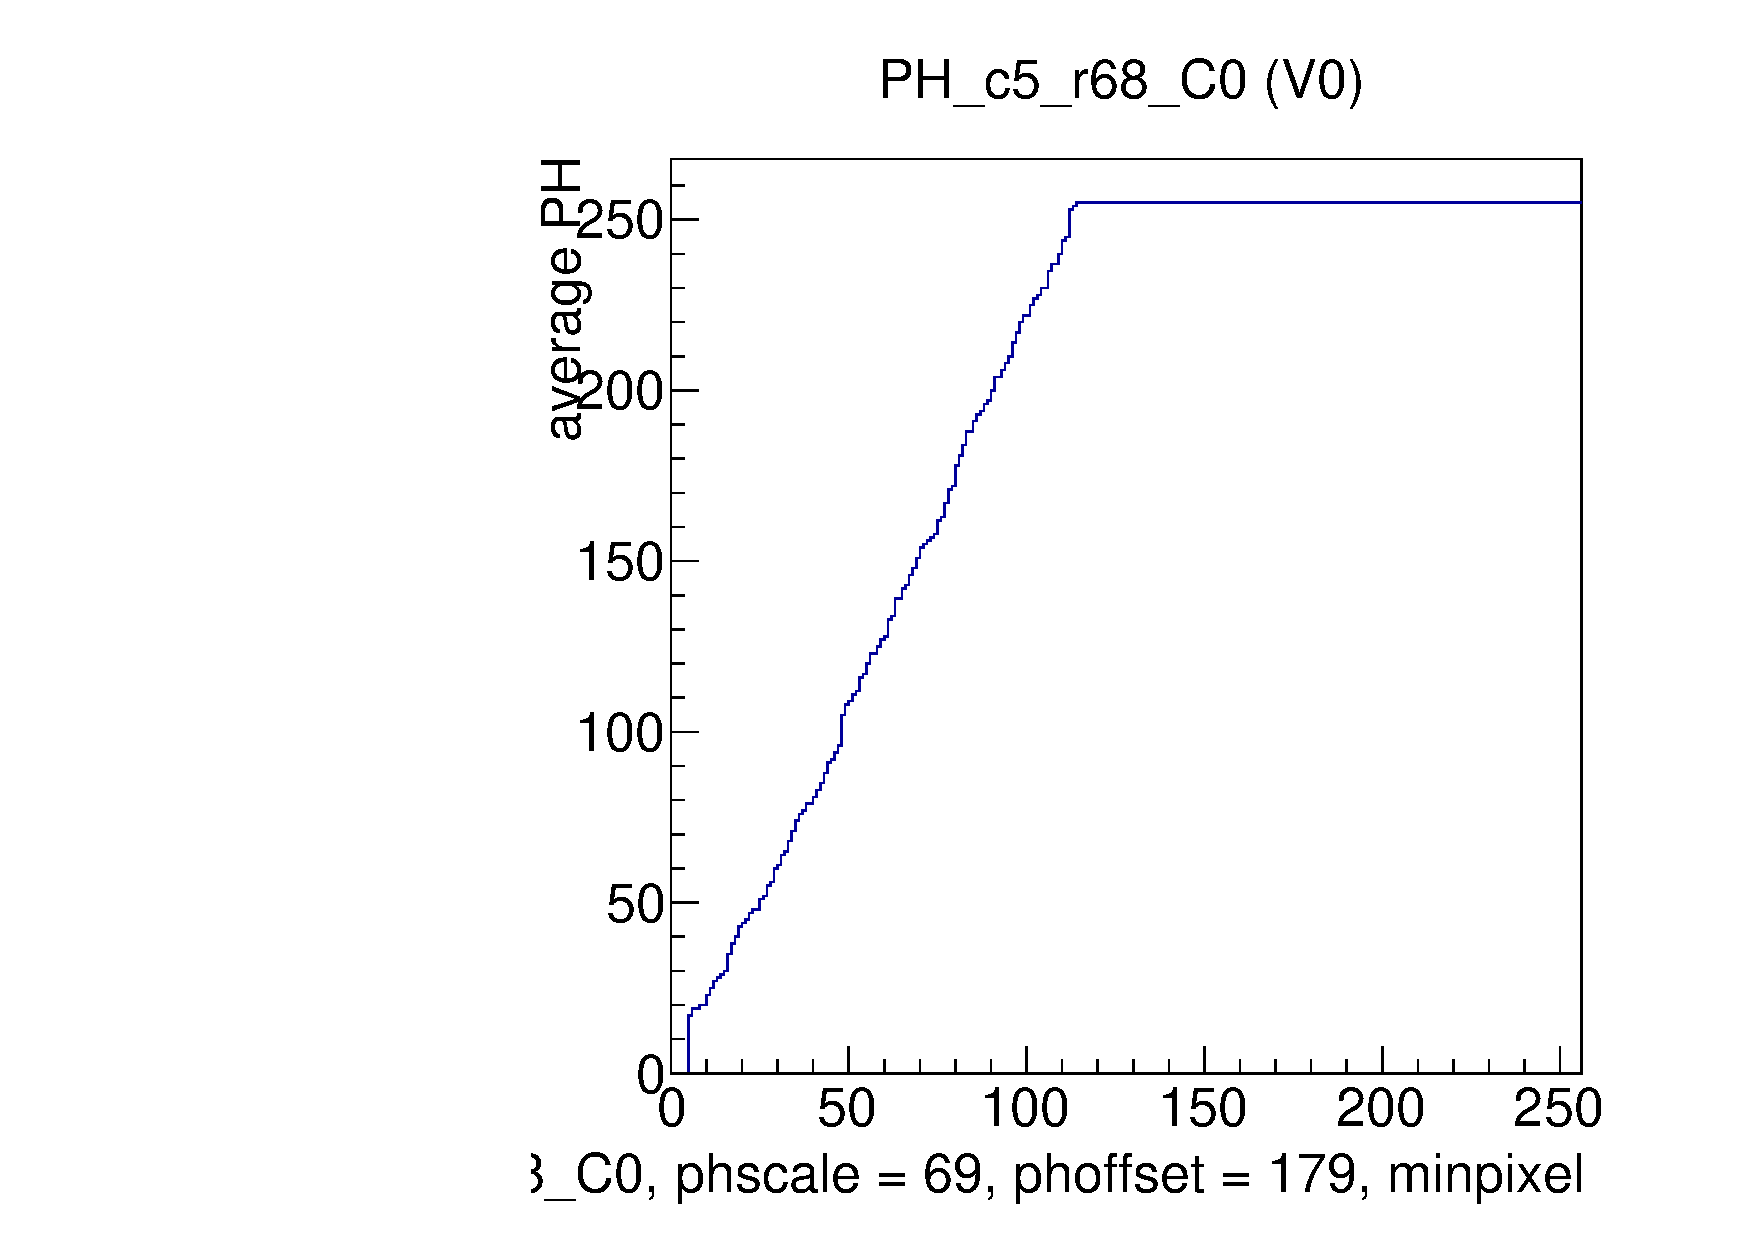
\includegraphics[width=1.0\textwidth]{figures/phopt_PH_c5_r68.pdf}
  \caption{PH vs. \vcal curve for previously identified low-gain pixel.}
  \label{fig:phopt_PH_c5_r68}
\end{minipage}
\hspace{0.3cm}
\begin{minipage}{0.45\textwidth}
  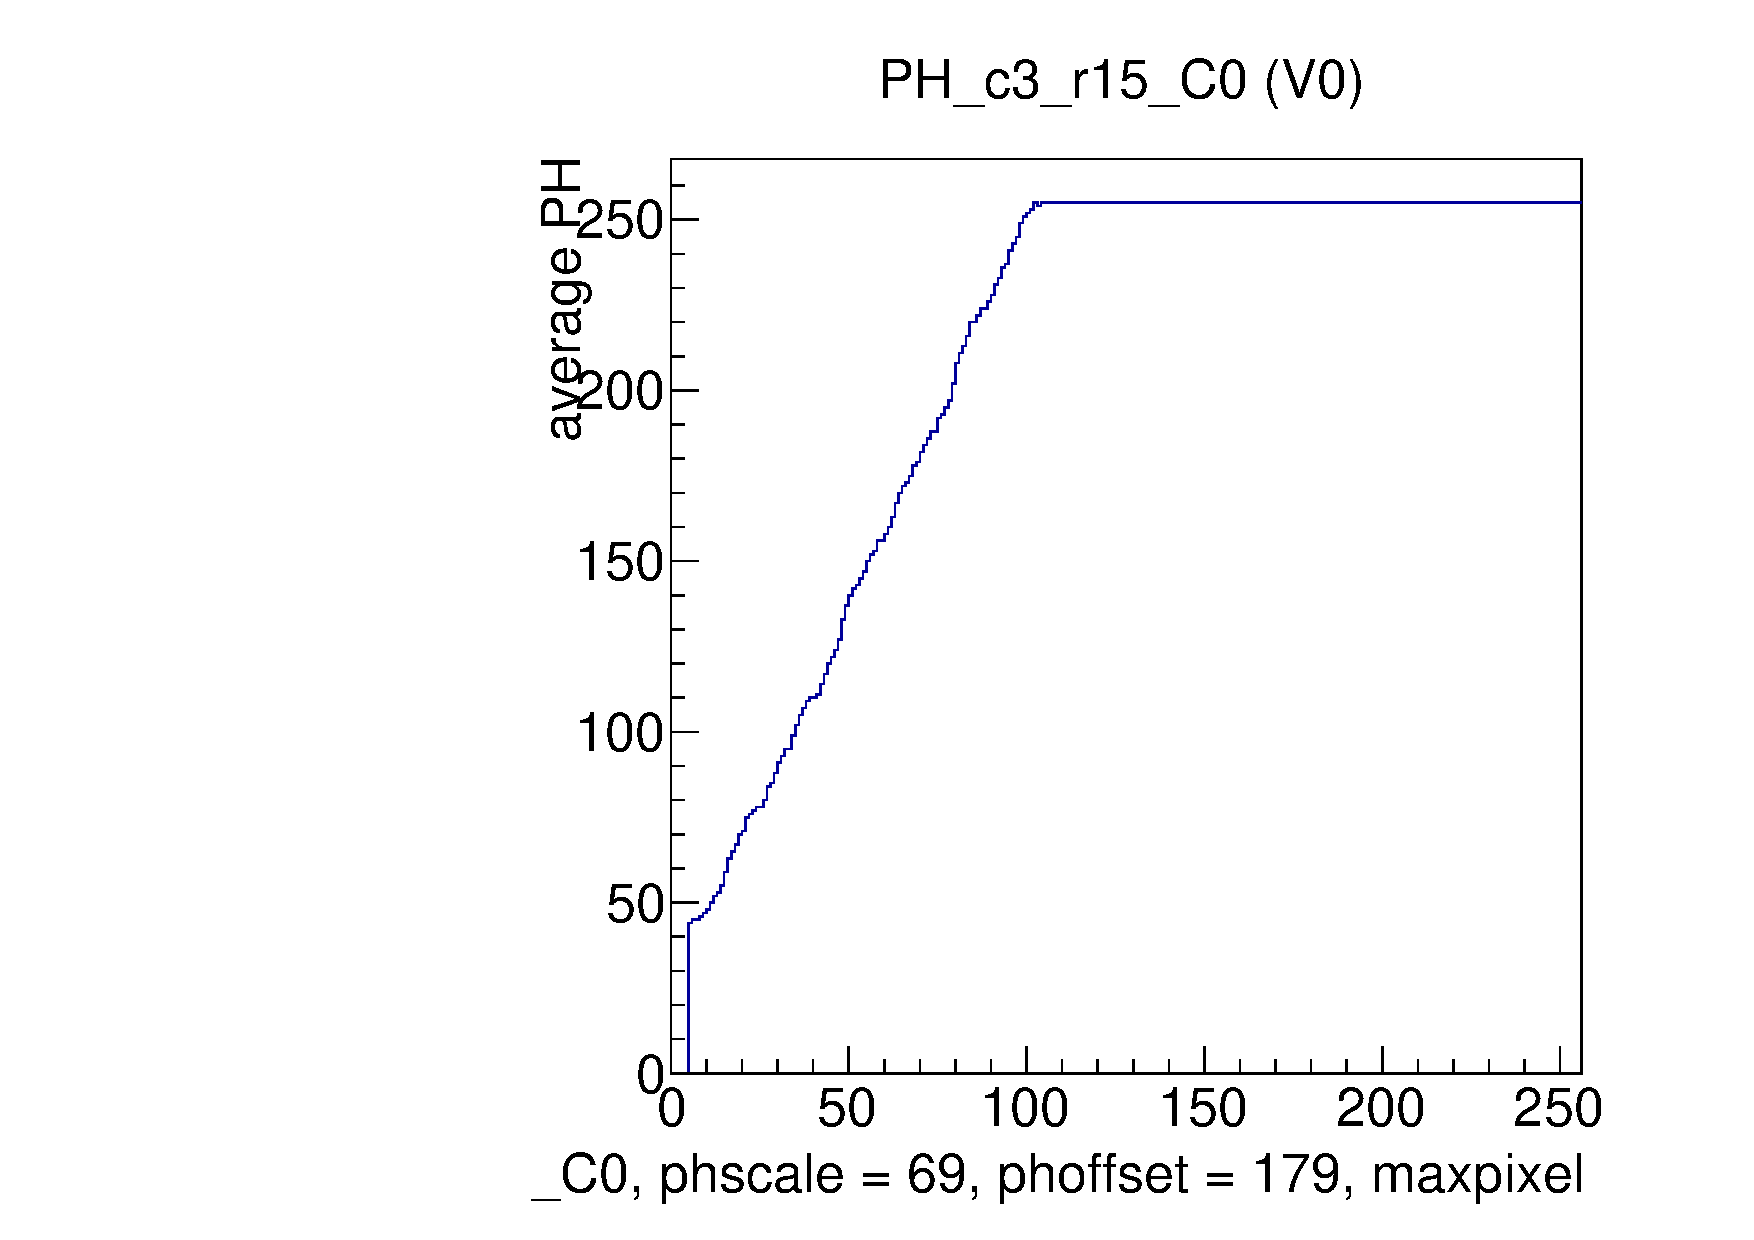
\includegraphics[width=1.0\textwidth]{figures/phopt_PH_c3_r15.pdf}
  \caption{PH vs. \vcal curve for previously identified high-gain pixel.}
  \label{fig:phopt_PH_c3_r15}
\end{minipage}
\end{figure}


% doing scans at three points in vcal

% done with Vcal set 10 units above turn-on for least sensitive pixel

\begin{figure}[!htp]
\centering
\begin{minipage}{0.45\textwidth}
  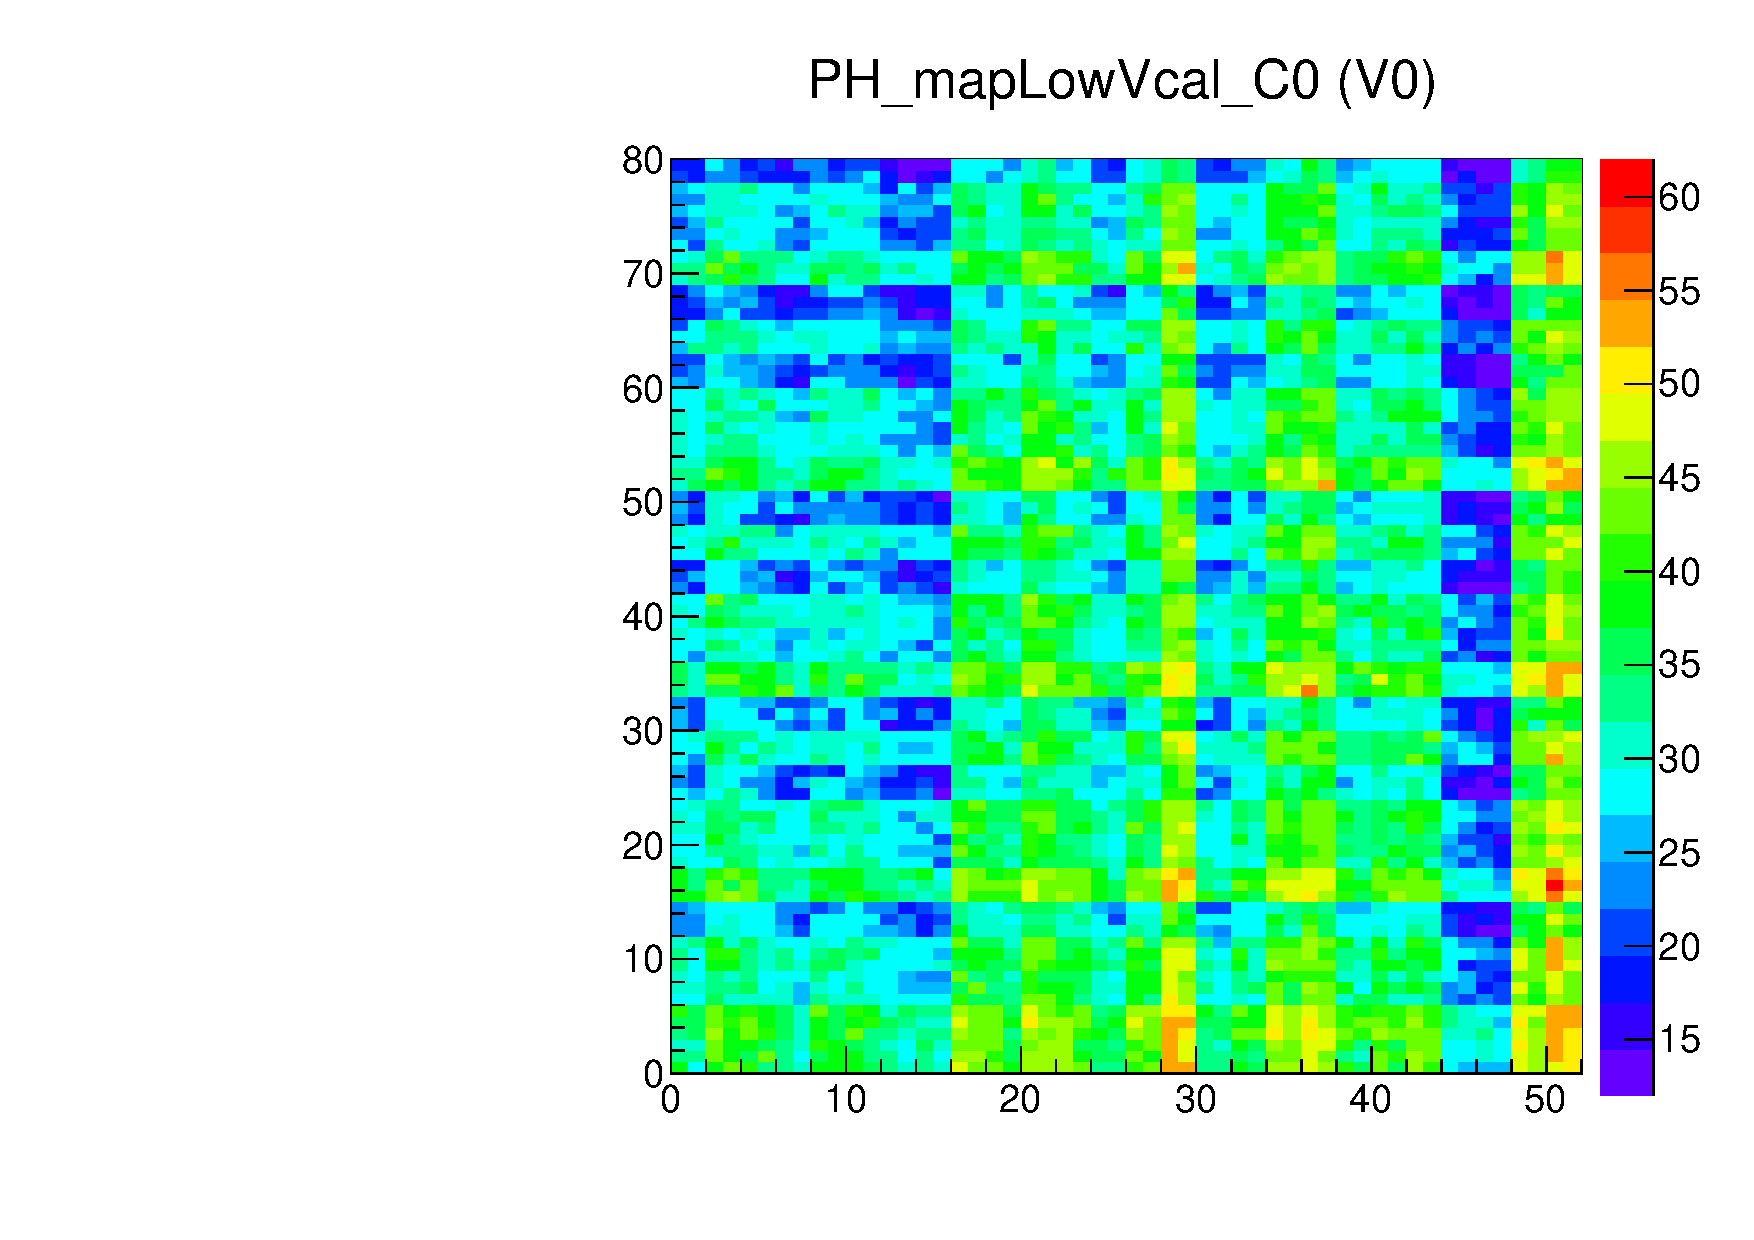
\includegraphics[width=1.0\textwidth]{figures/phopt_PH_mapLowVcal.pdf}
  \caption{\roc map of pulse heights with \vcal 10 units above minimum \vcal for low-gain pixel.}
  \label{fig:phopt_PH_mapLowVcal}
\end{minipage}
\hspace{0.3cm}
\begin{minipage}{0.45\textwidth}
  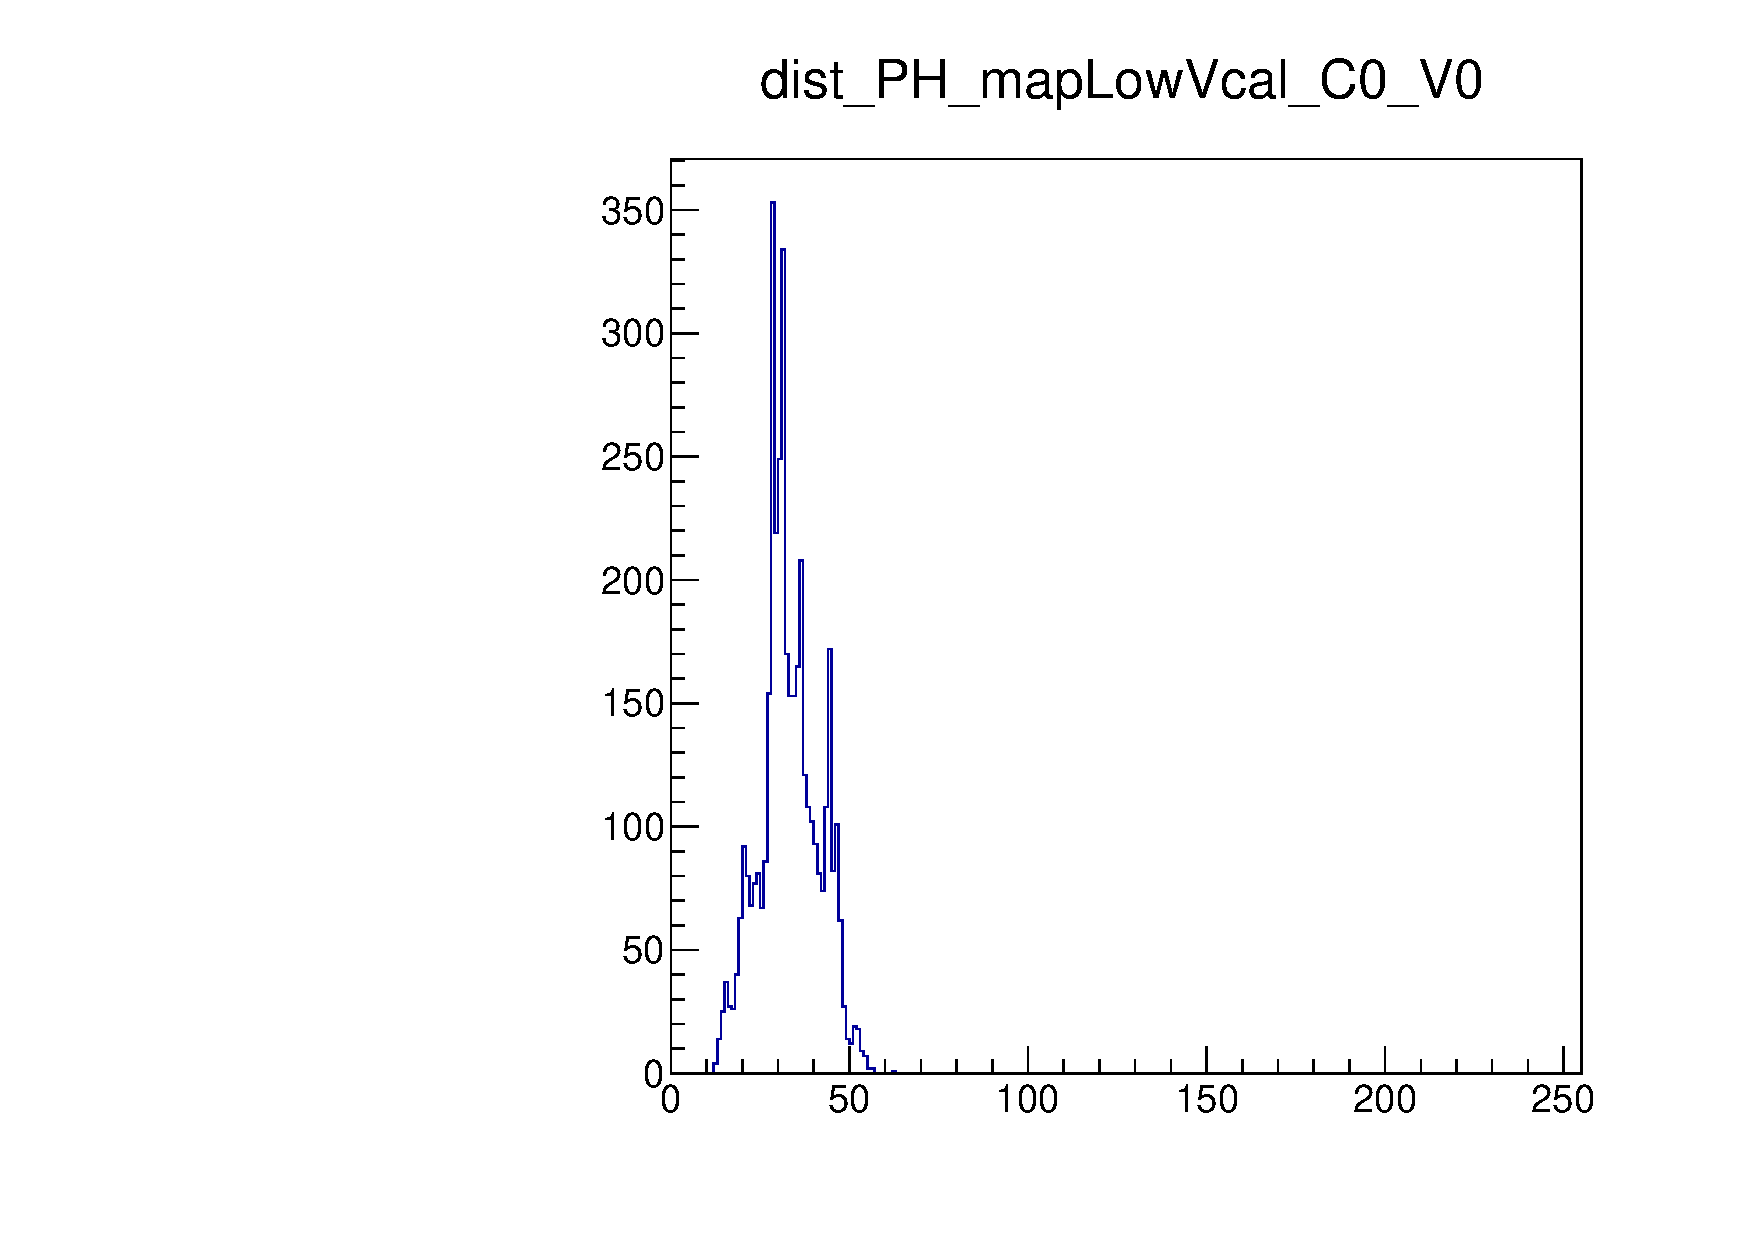
\includegraphics[width=1.0\textwidth]{figures/phopt_dist_PH_mapLowVcal.pdf}
  \caption{1D distribution of Figure~\ref{fig:phopt_PH_mapLowVcal}.}
  \label{fig:phopt_dist_PH_mapLowVcal}
\end{minipage}
\end{figure}

\begin{figure}[!htp]
\centering
\begin{minipage}{0.45\textwidth}
  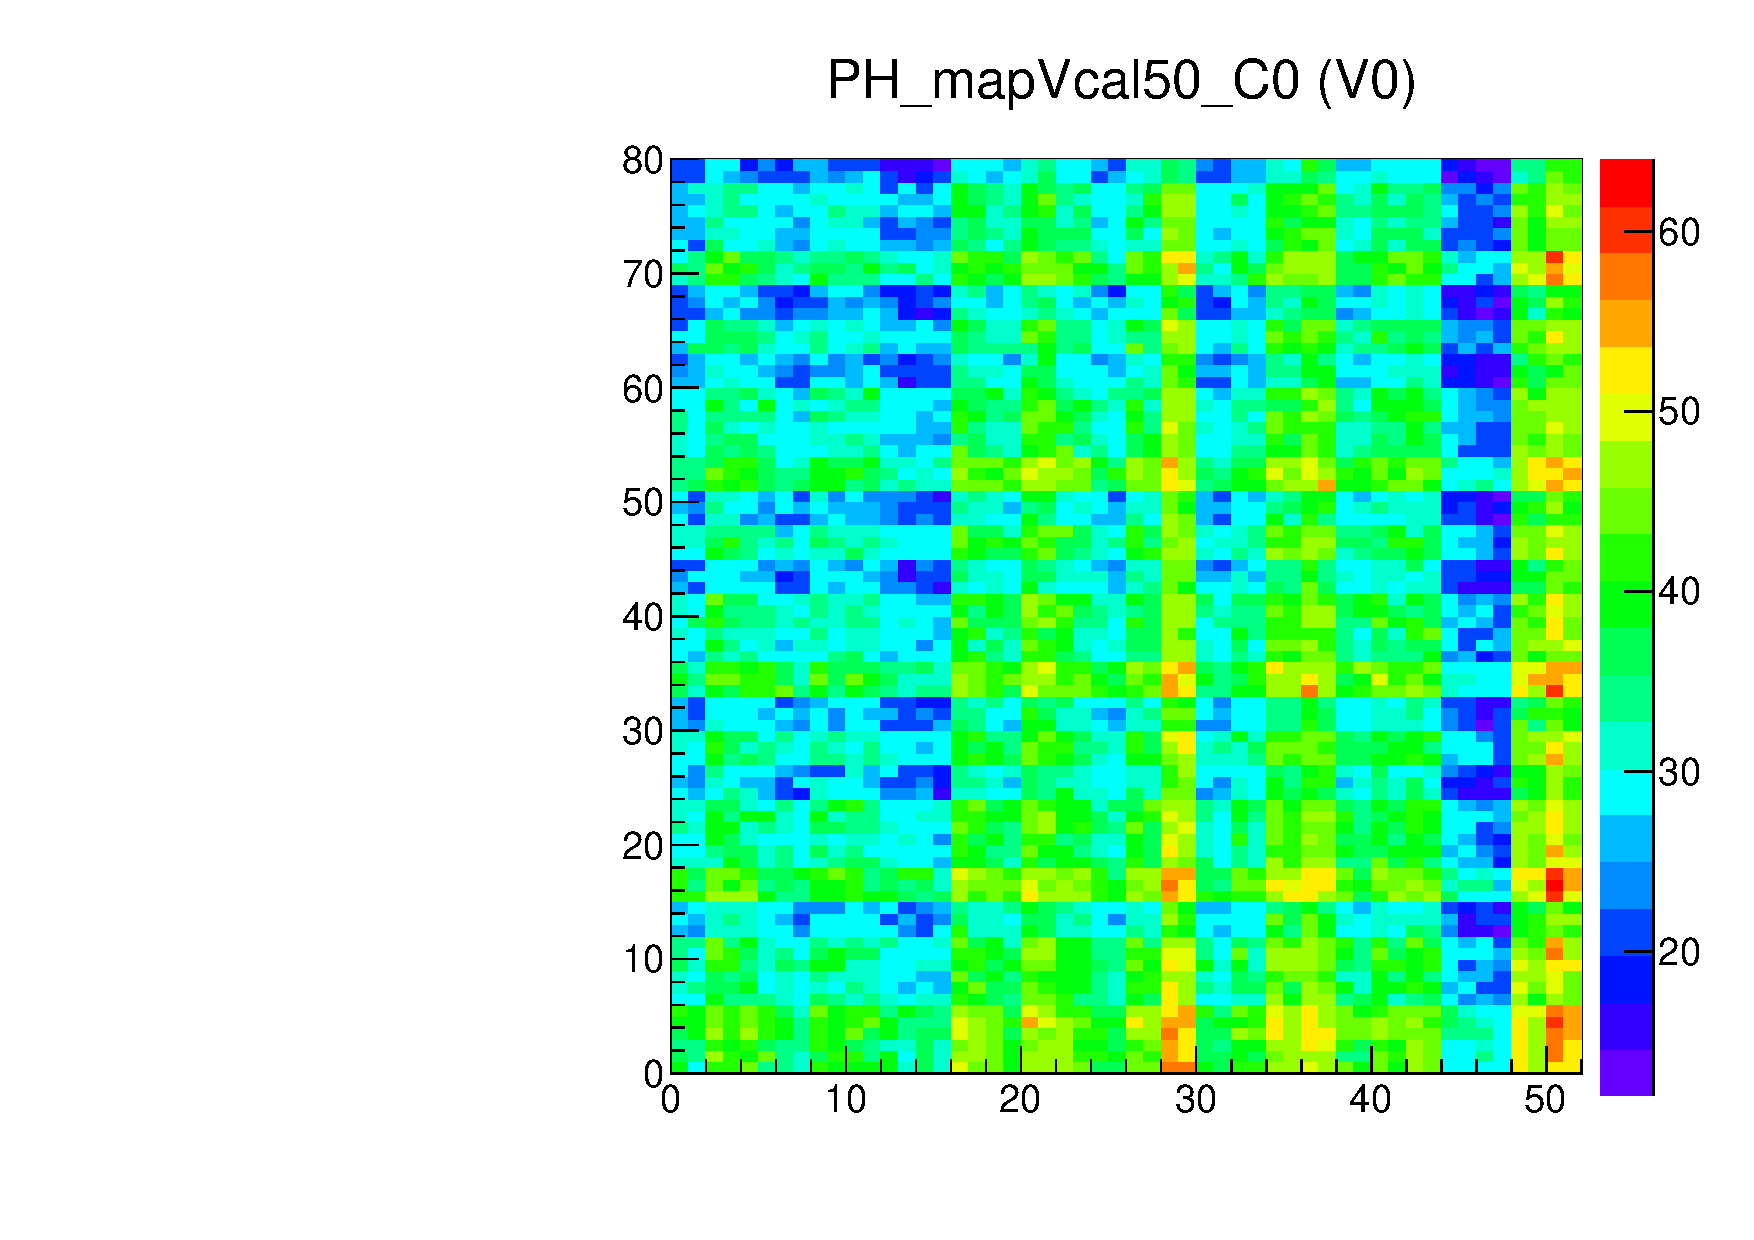
\includegraphics[width=1.0\textwidth]{figures/phopt_PH_mapVcal50.pdf}
  \caption{\roc map of pulse heights with \vcal=50 (low range).}
  \label{fig:phopt_PH_mapVcal50}
\end{minipage}
\hspace{0.3cm}
\begin{minipage}{0.45\textwidth}
  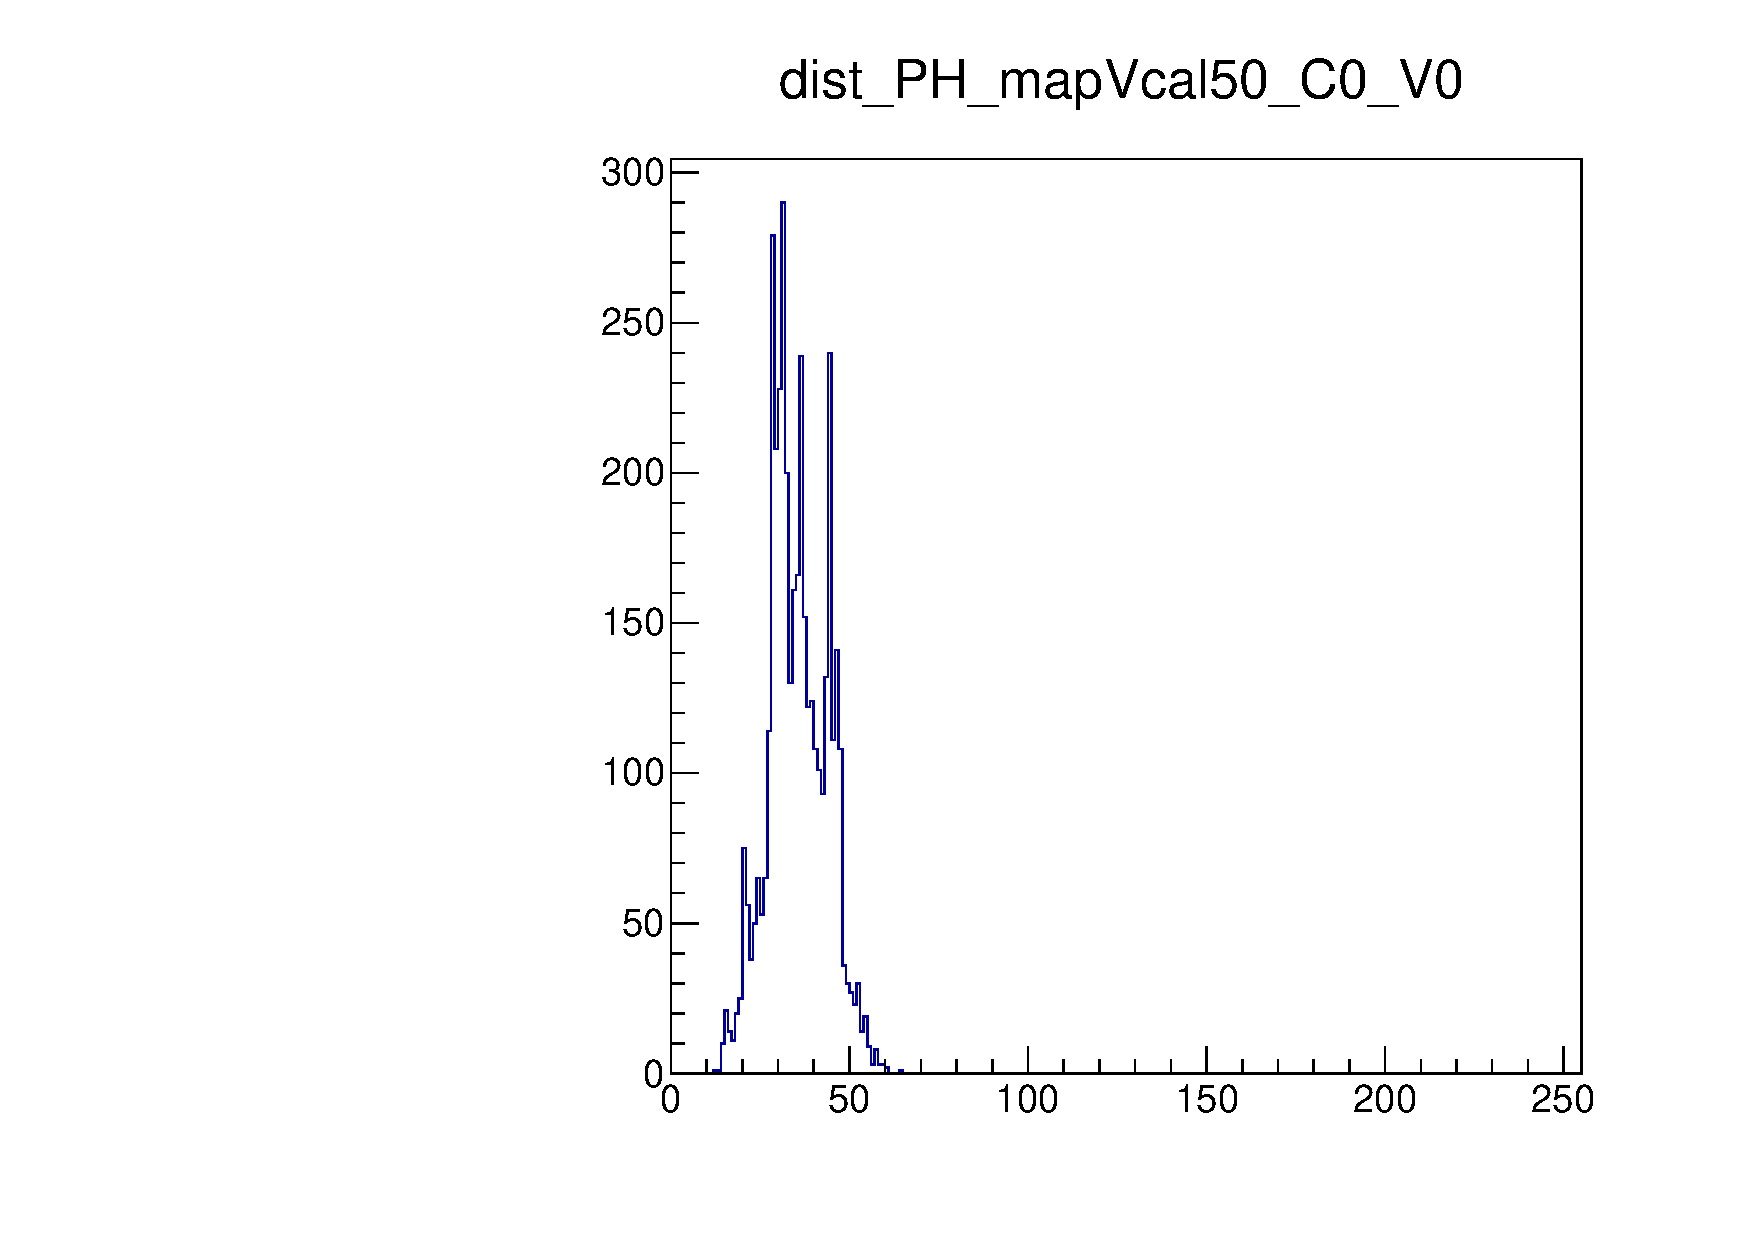
\includegraphics[width=1.0\textwidth]{figures/phopt_dist_PH_mapVcal50.pdf}
  \caption{1D distribution of Figure~\ref{fig:phopt_PH_mapVcal50}.}
  \label{fig:phopt_dist_PH_mapVcal50}
\end{minipage}
\end{figure}

% done at user-defined target saturation Vcal - default 100 (high range)

\begin{figure}[!htp]
\centering
\begin{minipage}{0.45\textwidth}
  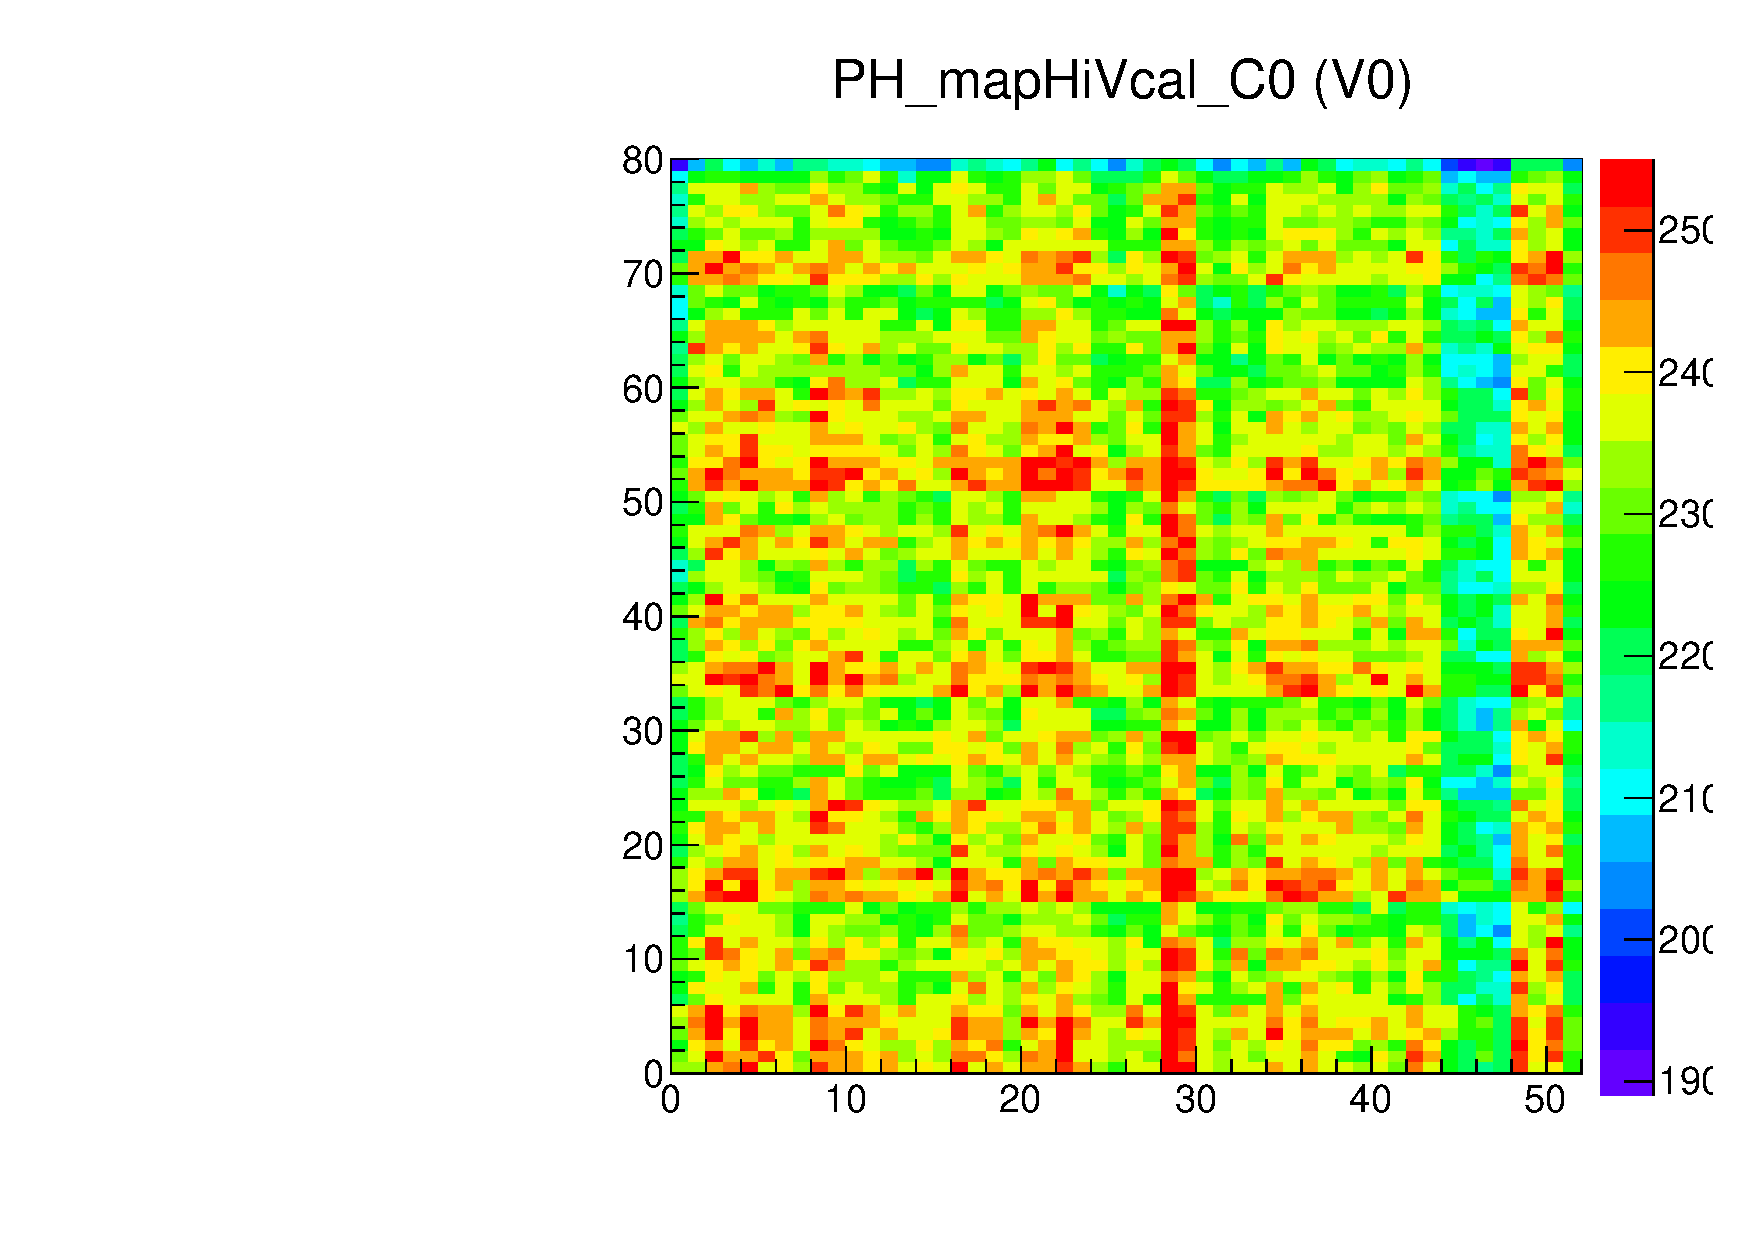
\includegraphics[width=1.0\textwidth]{figures/phopt_PH_mapHiVcal.pdf}
  \caption{\roc map of pulse heights with \vcal set to target ADC saturation point.}
  \label{fig:phopt_PH_mapHiVcal}
\end{minipage}
\hspace{0.3cm}
\begin{minipage}{0.45\textwidth}
  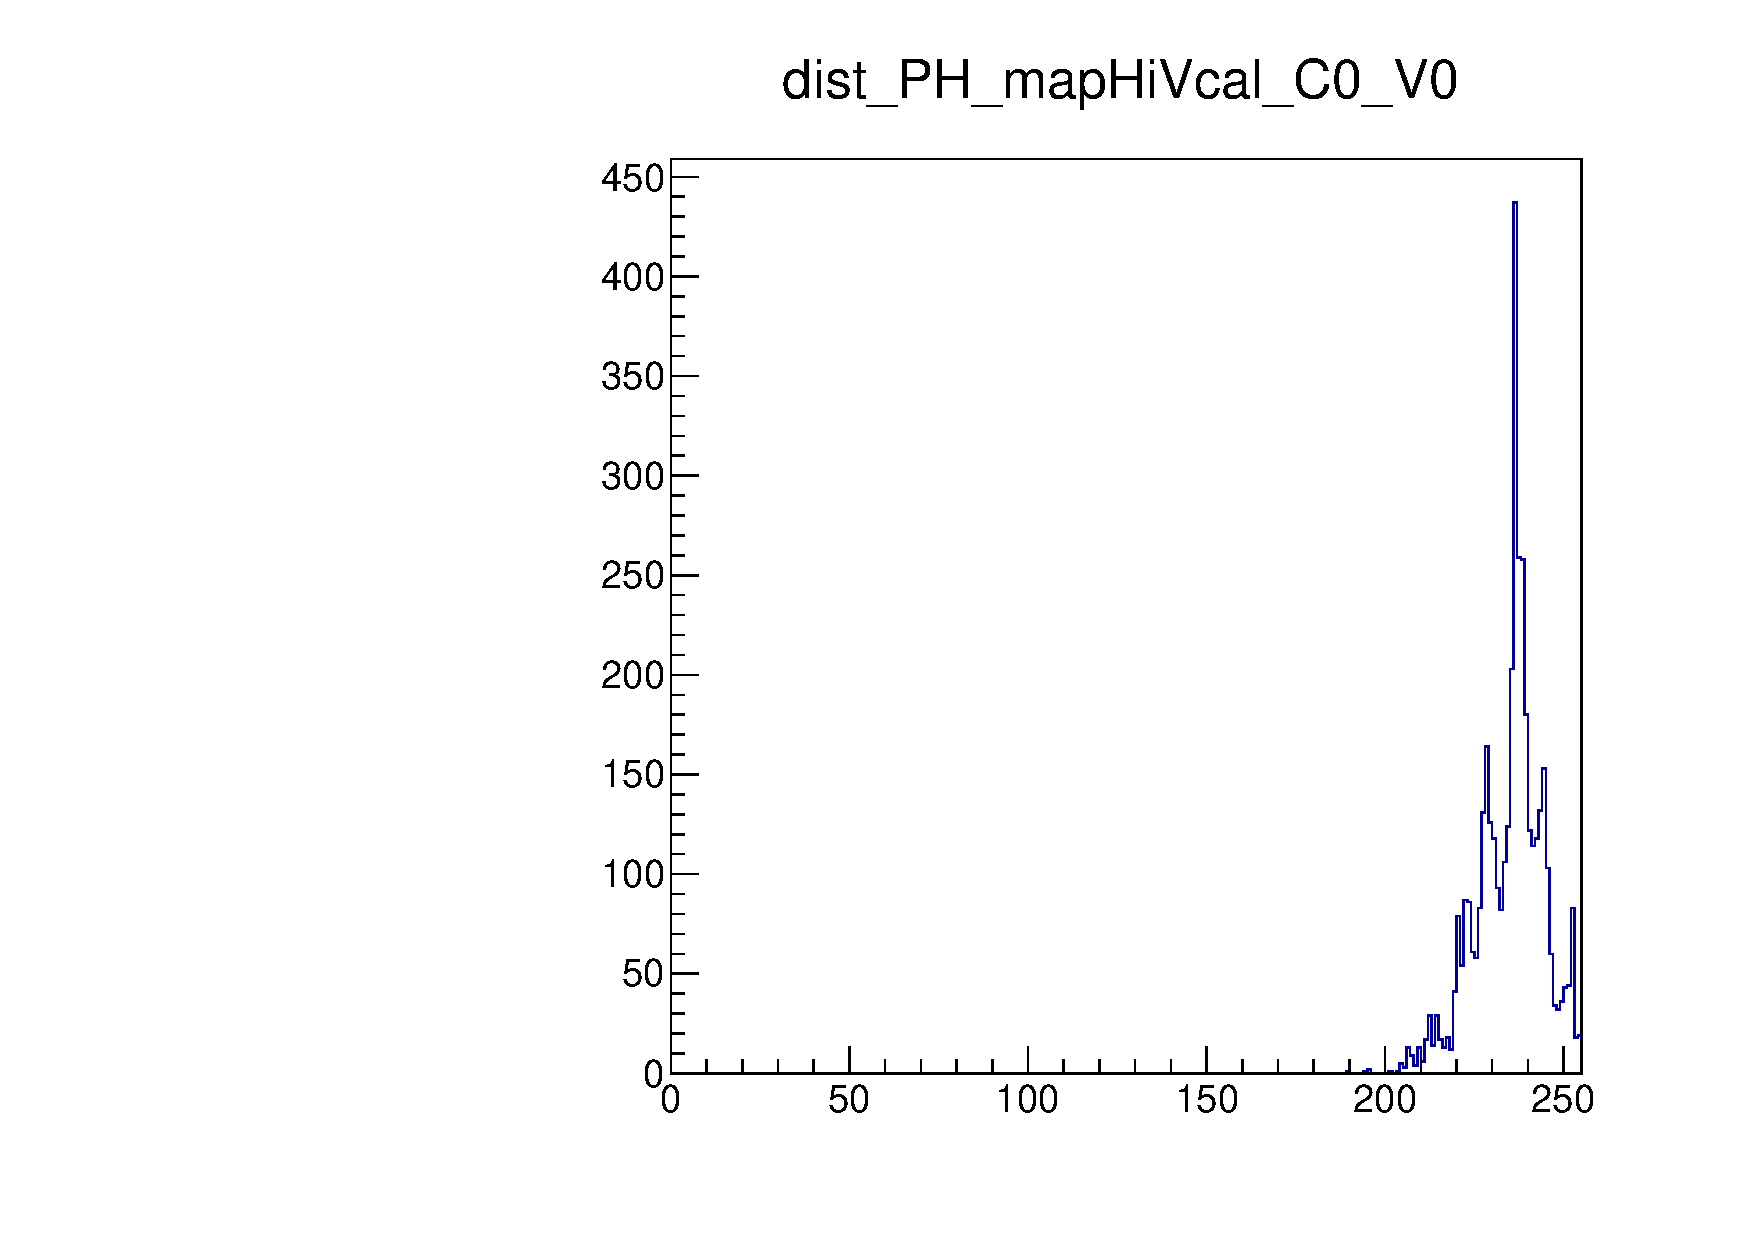
\includegraphics[width=1.0\textwidth]{figures/phopt_dist_PH_mapHiVcal.pdf}
  \caption{1D distribution of Figure~\ref{fig:phopt_PH_mapHiVcal}.}
  \label{fig:phopt_dist_PH_mapHiVcal}
\end{minipage}
\end{figure}



% ----------------------------------------------------------------------

\newpage

\subsection{\gainped Test}
\label{ss:gainped}

\subsubsection{Purpose}

The \gainped test does not alter any \dac parameters,
but merely evaluates the shape of the pulse height vs. \vcal distribution for each pixel.
For each pixel, th distribution is fitted and the fit parameters are stored for later use.
Since variations in gain are expected between pixels in a \roc,
the gain must be measured independantly for each pixel so that the pulse height to be calibrated back to the input signal size, 
in units of the \vcal~\dac (high range).

\subsubsection{\textcolor{red}{Methodology}}
\subsubsection{Output}

\begin{figure}[!Hp]
\centering
\begin{minipage}{0.45\textwidth}
  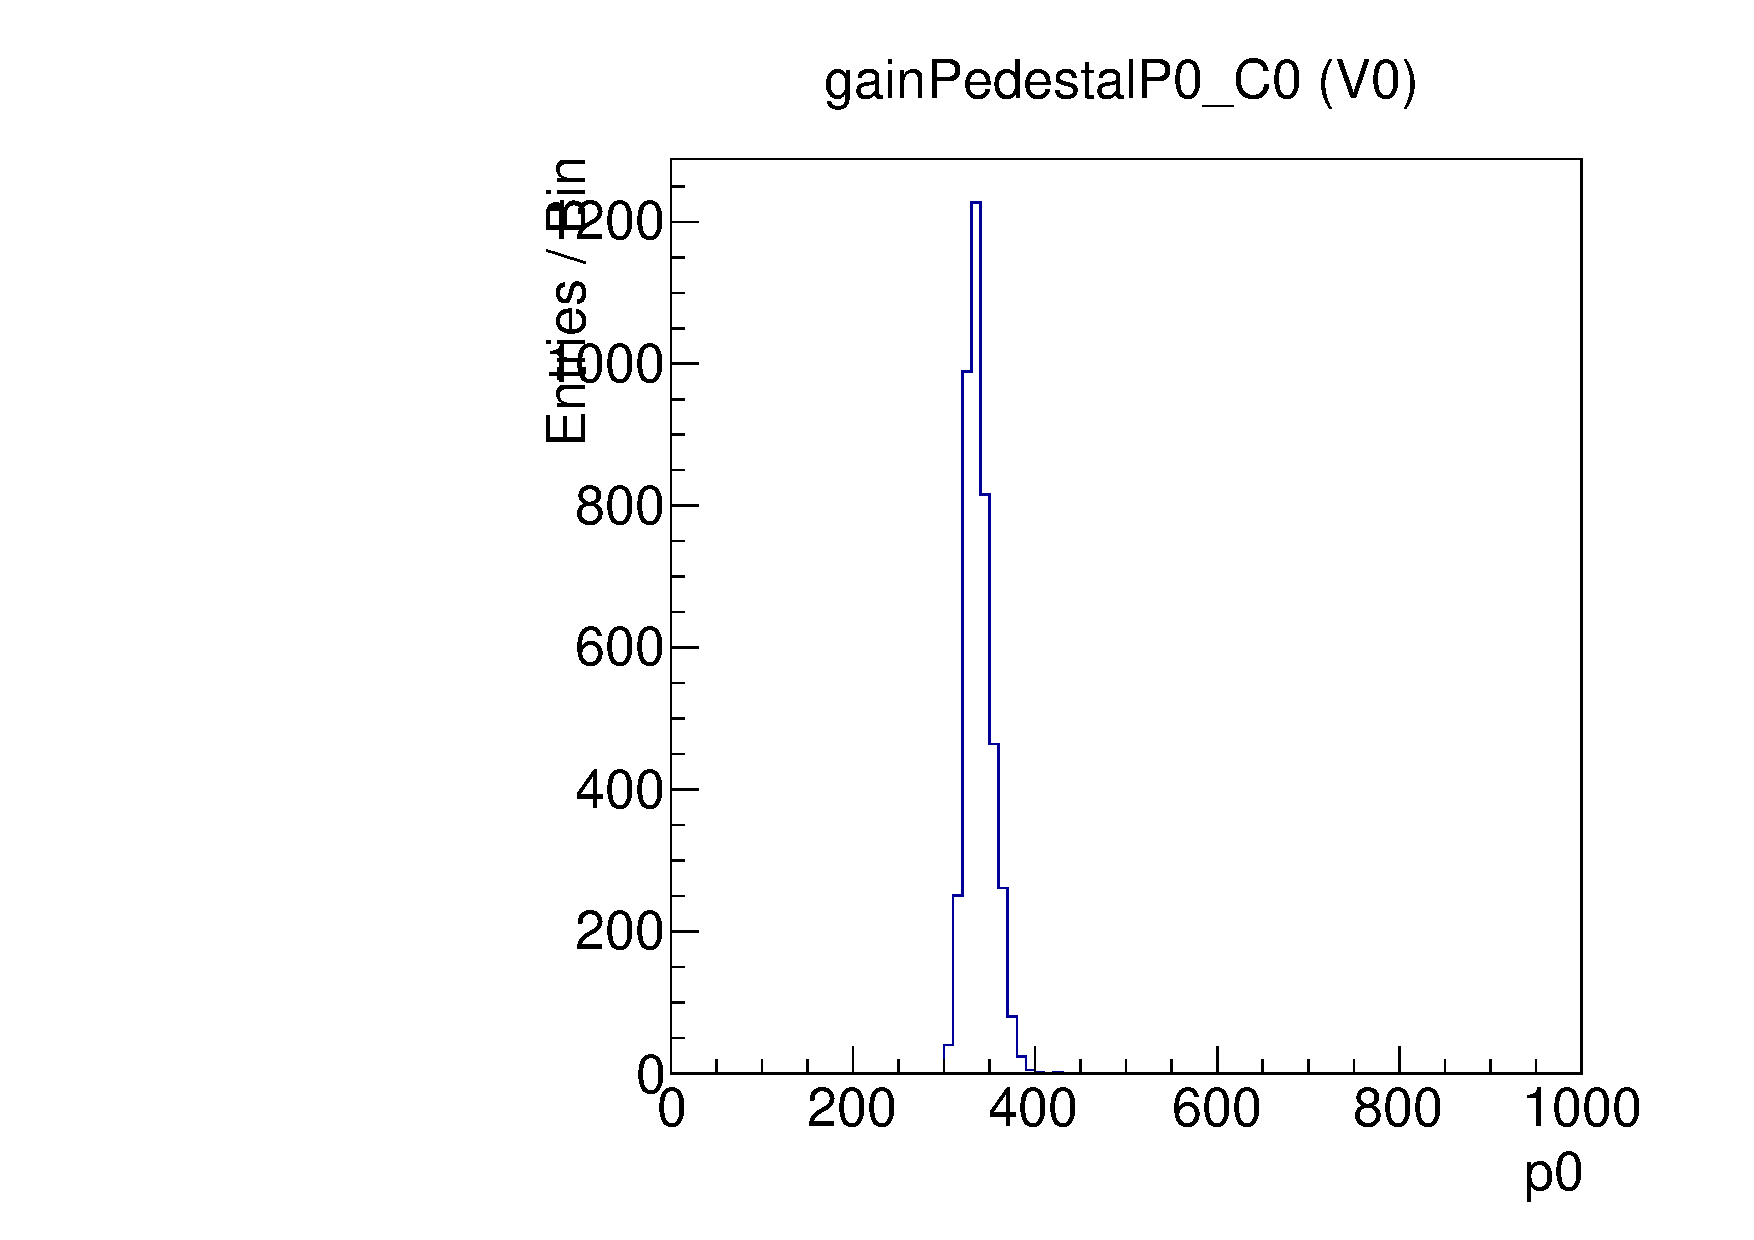
\includegraphics[width=1.0\textwidth]{figures/gainped_gainPedestalP0.pdf}
  \caption{}
  \label{fig:gainped_gainPedestalP0}
\end{minipage}
\hspace{0.3cm}
\begin{minipage}{0.45\textwidth}
  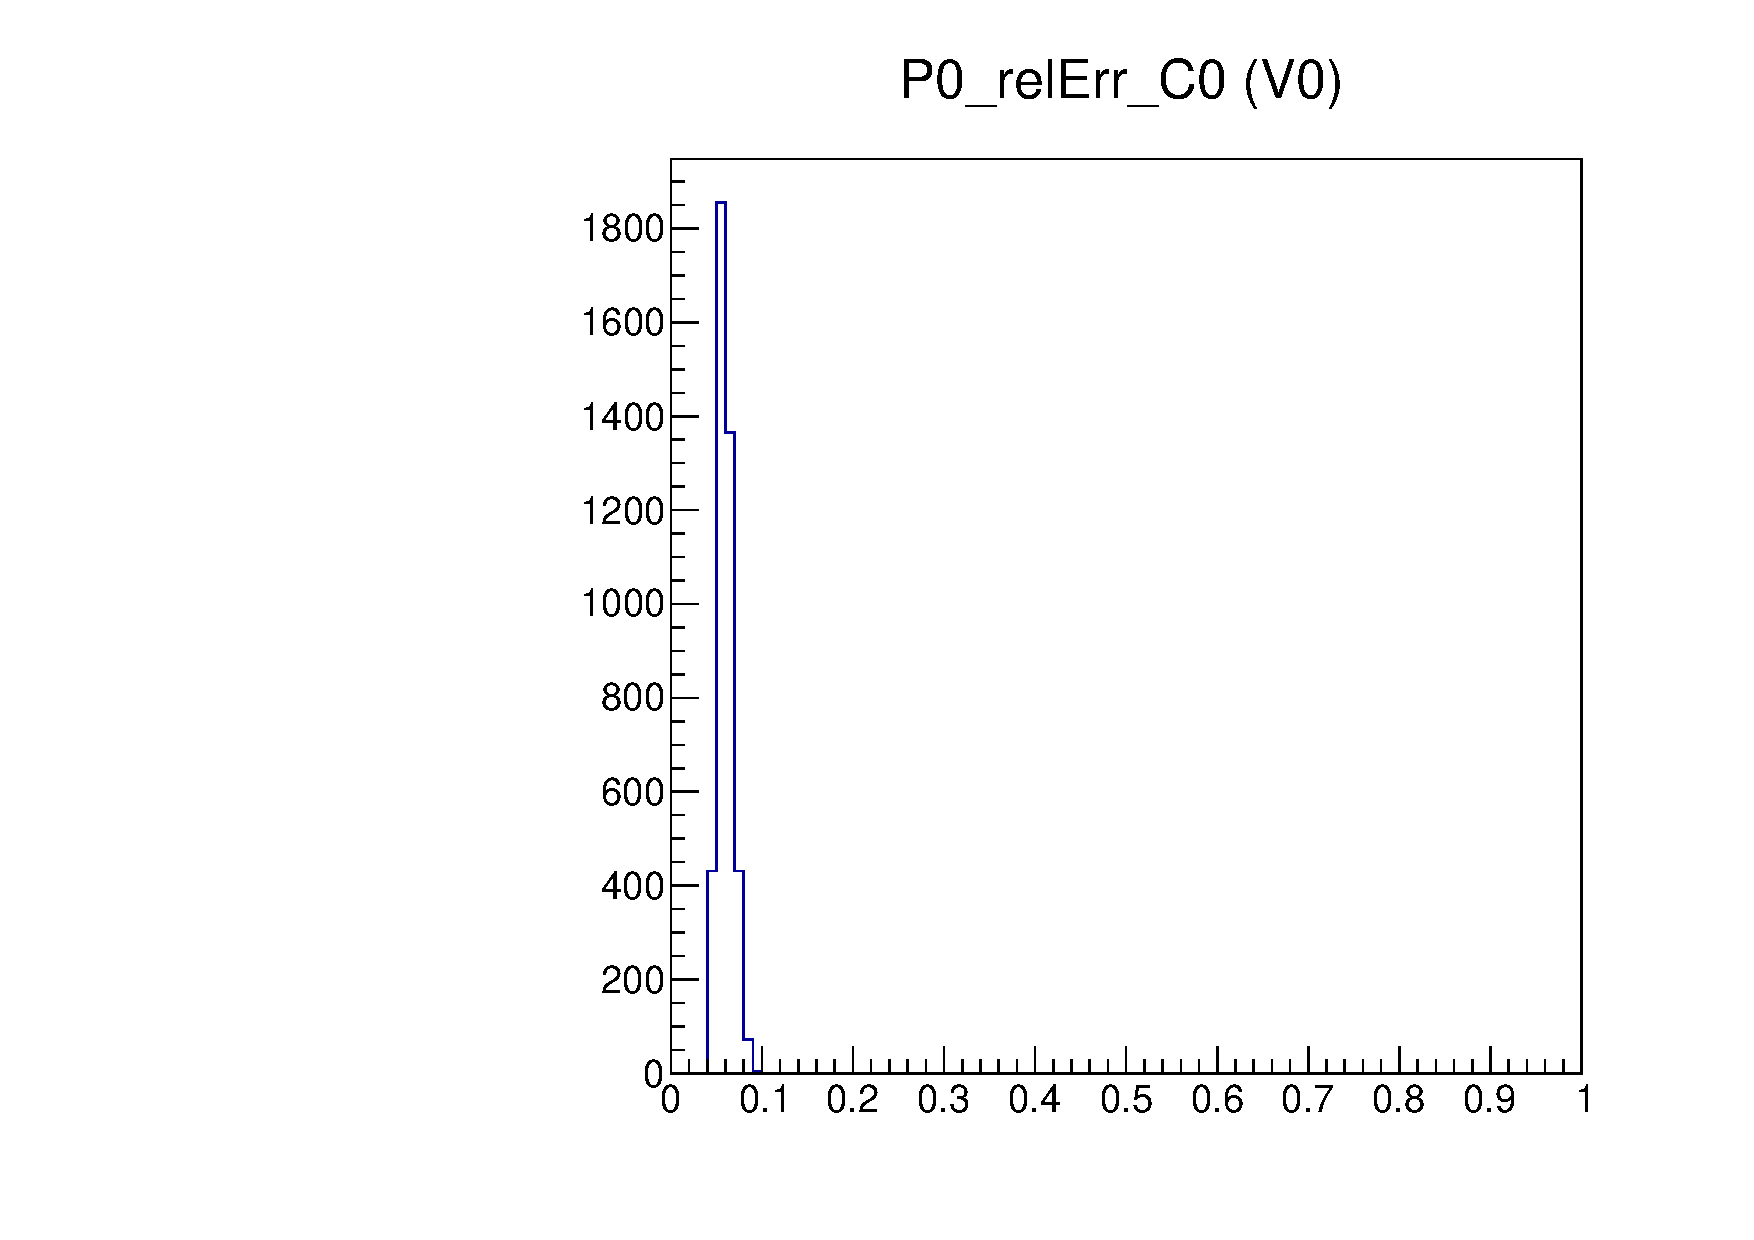
\includegraphics[width=1.0\textwidth]{figures/gainped_P0_relErr.pdf}
  \caption{}
  \label{fig:gainped_P0_relErr}
\end{minipage}
\end{figure}

\begin{figure}[!Hp]
\centering
\begin{minipage}{0.45\textwidth}
  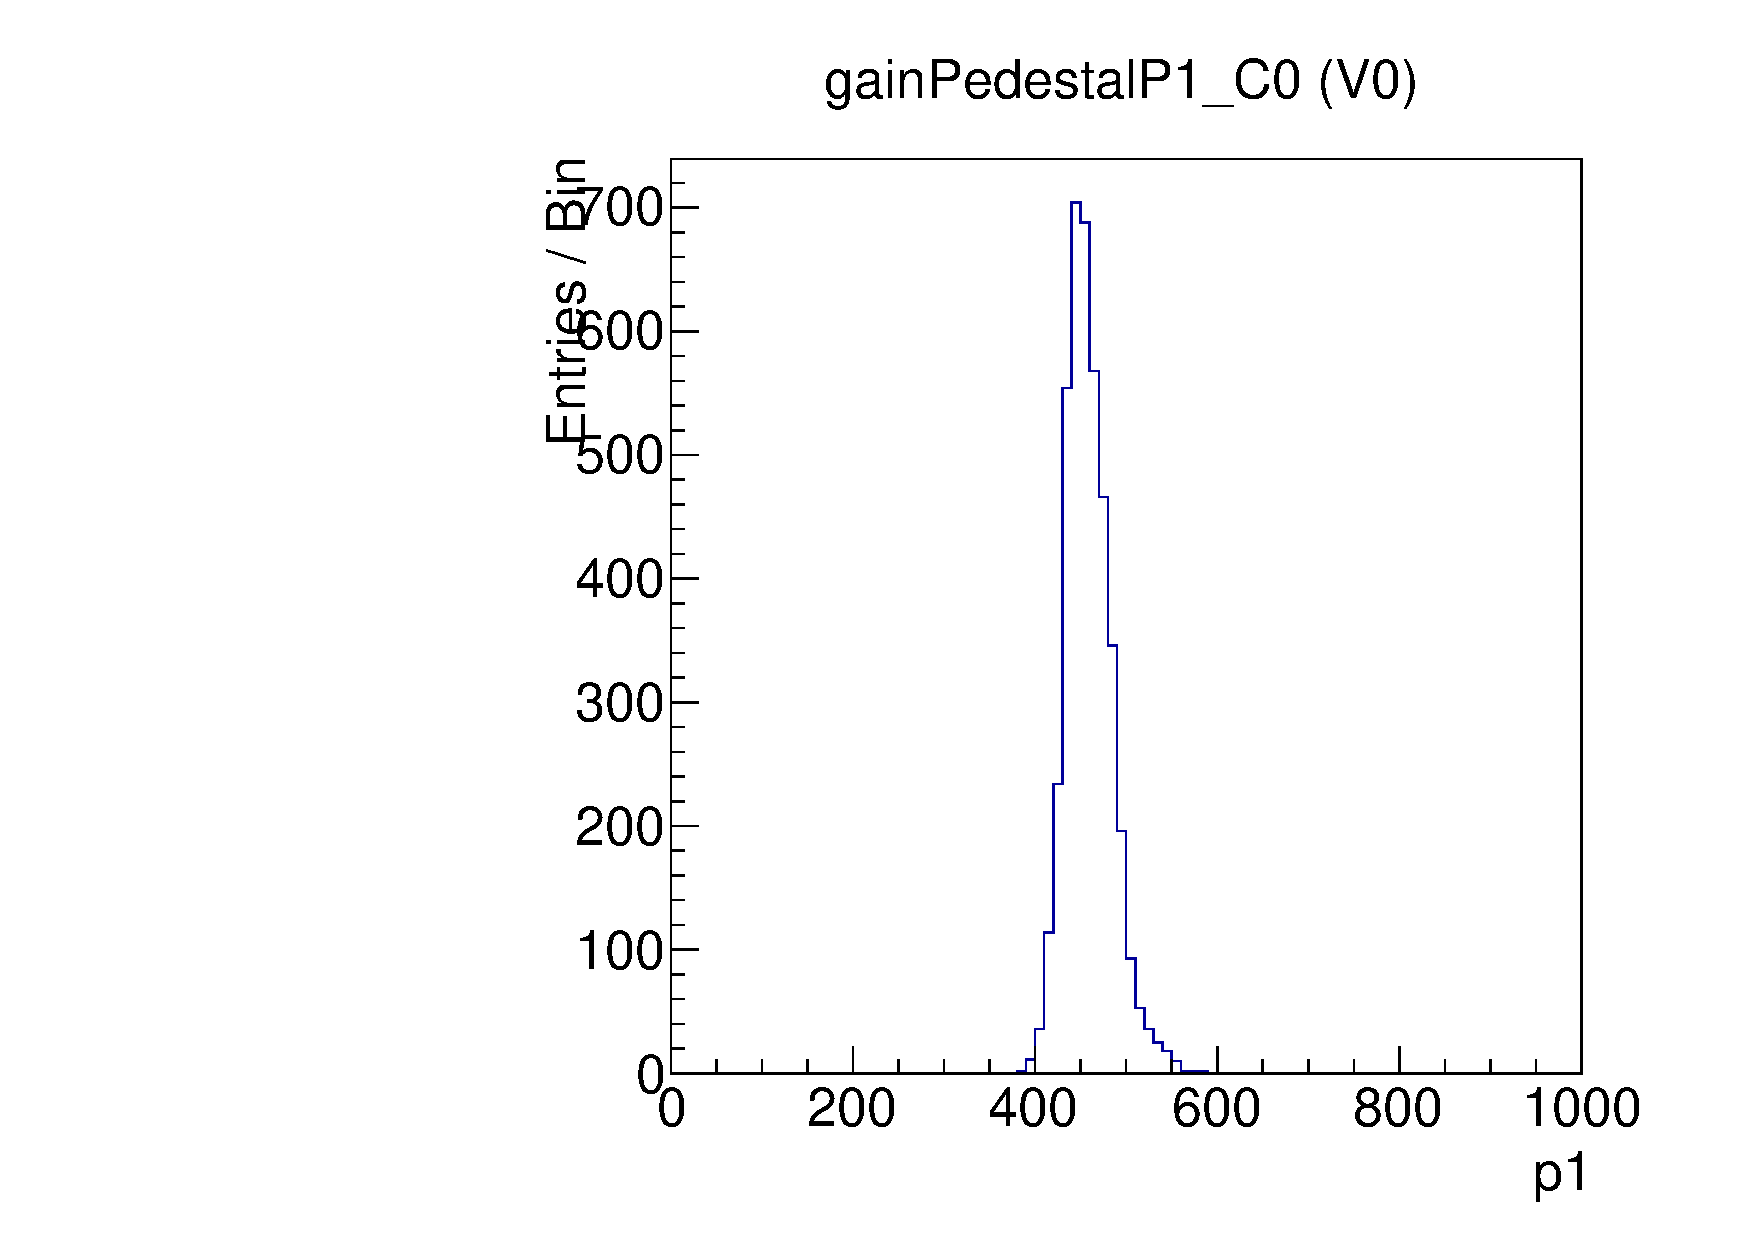
\includegraphics[width=1.0\textwidth]{figures/gainped_gainPedestalP1.pdf}
  \caption{}
  \label{fig:gainped_gainPedestalP1}
\end{minipage}
\hspace{0.3cm}
\begin{minipage}{0.45\textwidth}
  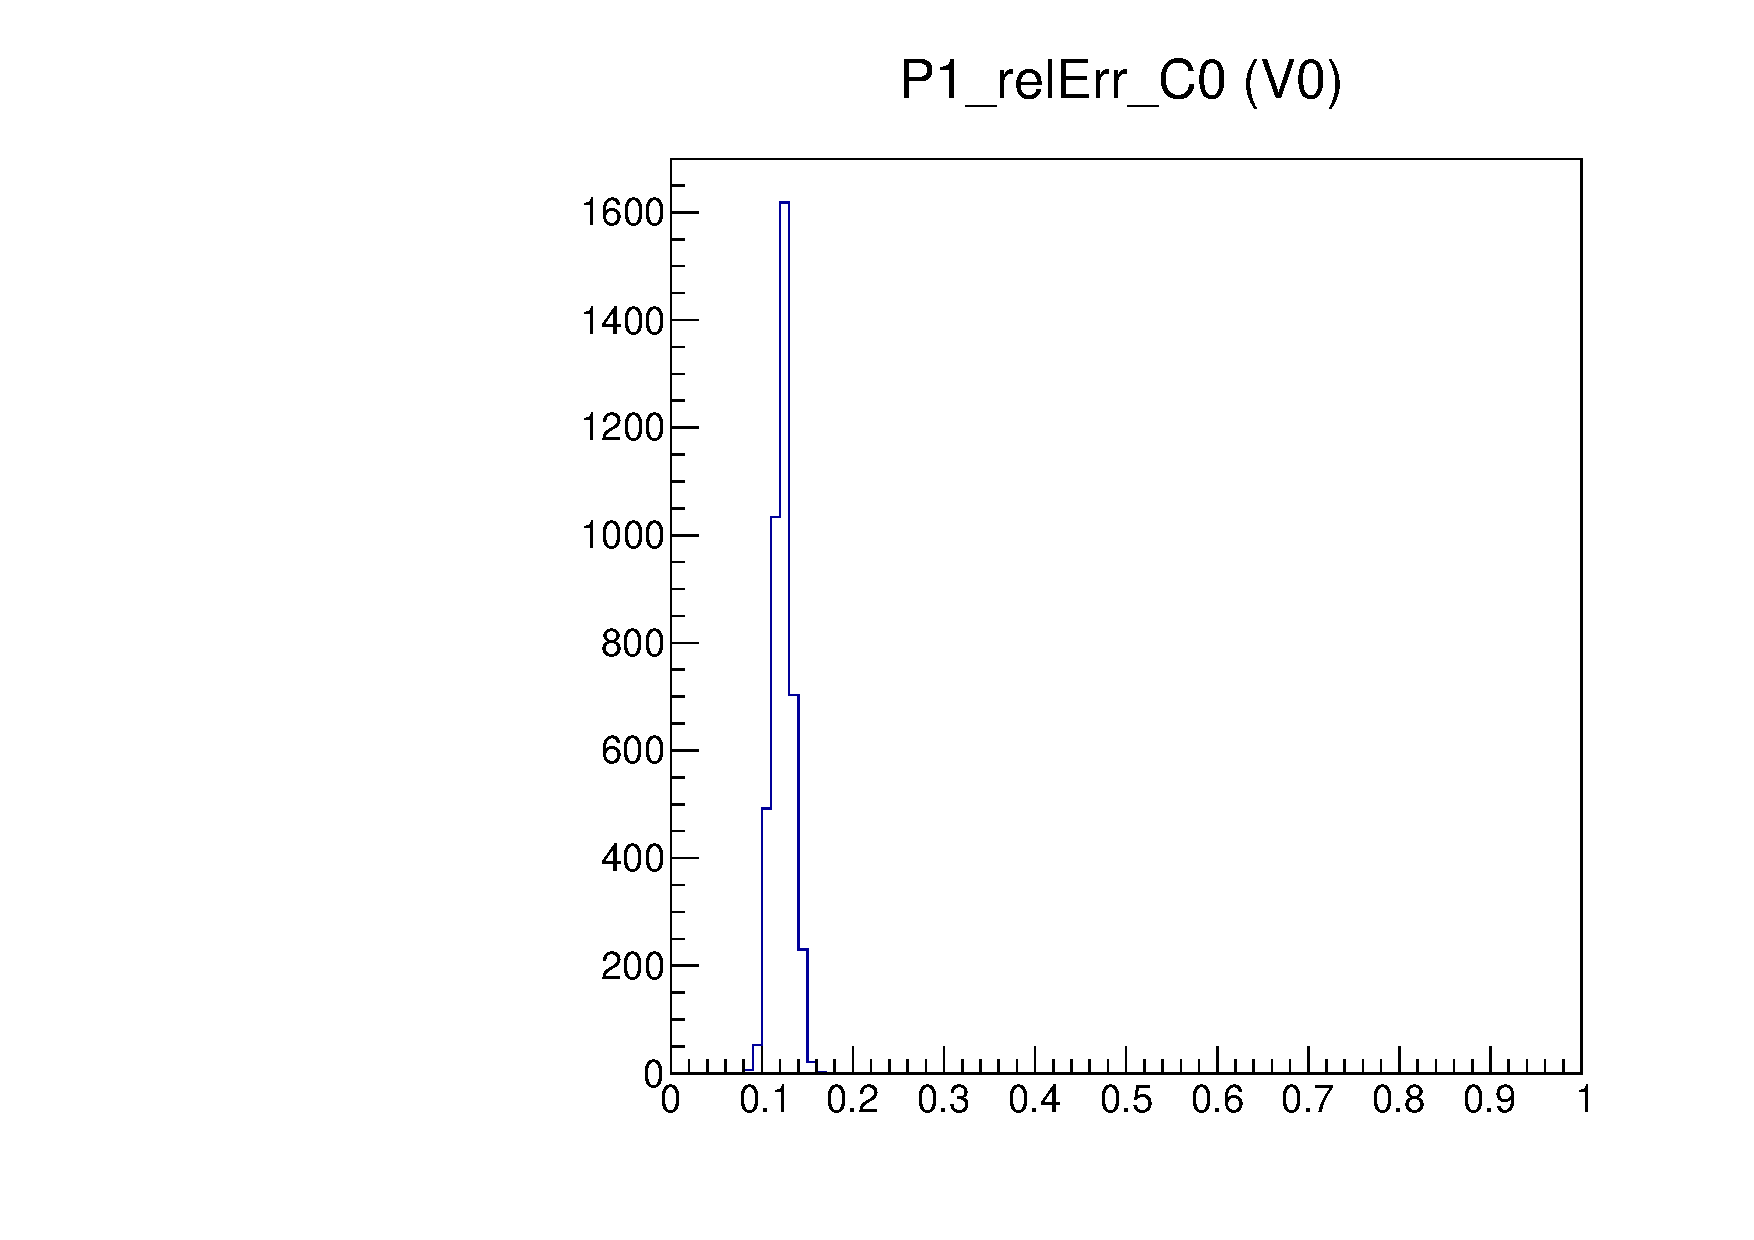
\includegraphics[width=1.0\textwidth]{figures/gainped_P1_relErr.pdf}
  \caption{}
  \label{fig:gainped_P1_relErr}
\end{minipage}
\end{figure}

\begin{figure}[!Hp]
\centering
\begin{minipage}{0.45\textwidth}
  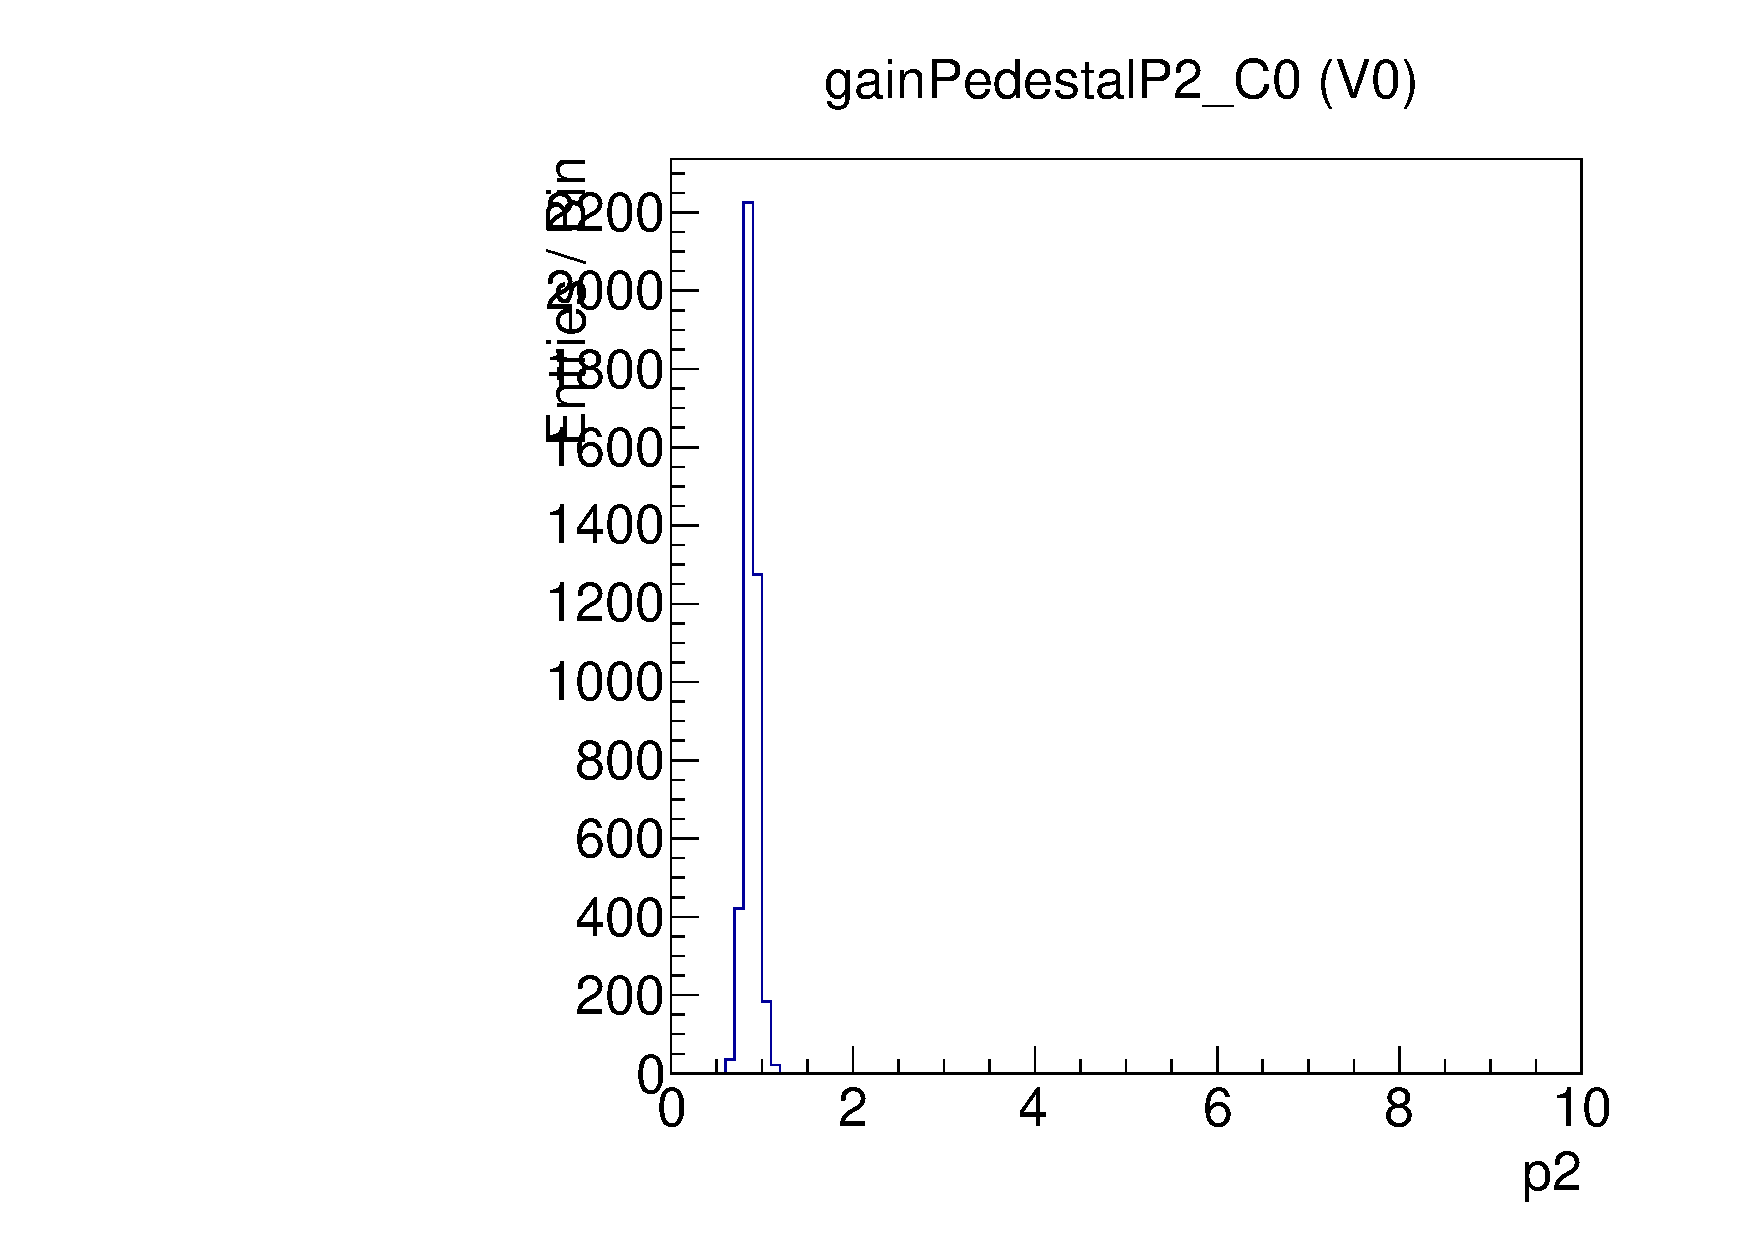
\includegraphics[width=1.0\textwidth]{figures/gainped_gainPedestalP2.pdf}
  \caption{}
  \label{fig:gainped_gainPedestalP2}
\end{minipage}
\hspace{0.3cm}
\begin{minipage}{0.45\textwidth}
  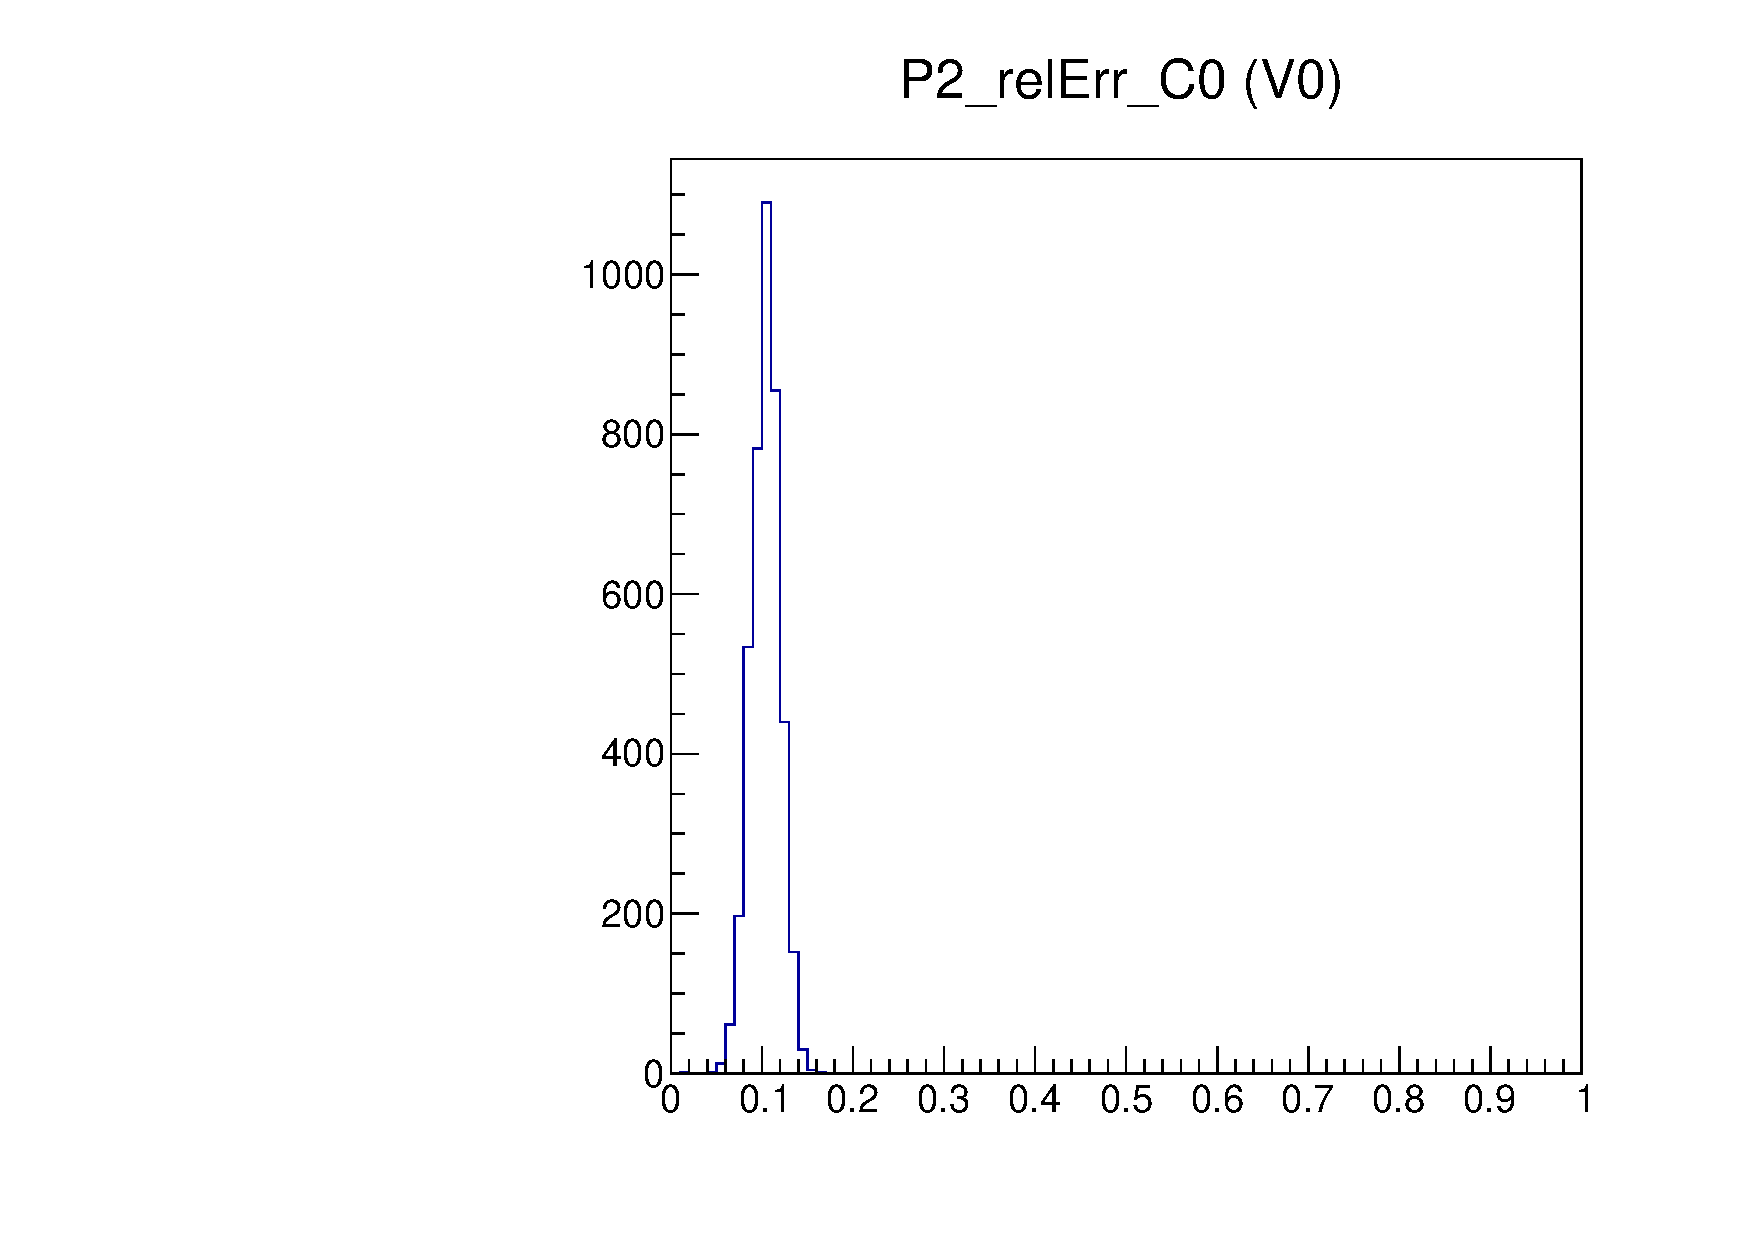
\includegraphics[width=1.0\textwidth]{figures/gainped_P2_relErr.pdf}
  \caption{}
  \label{fig:gainped_P2_relErr}
\end{minipage}
\end{figure}

\begin{figure}[!Hp]
\centering
\begin{minipage}{0.45\textwidth}
  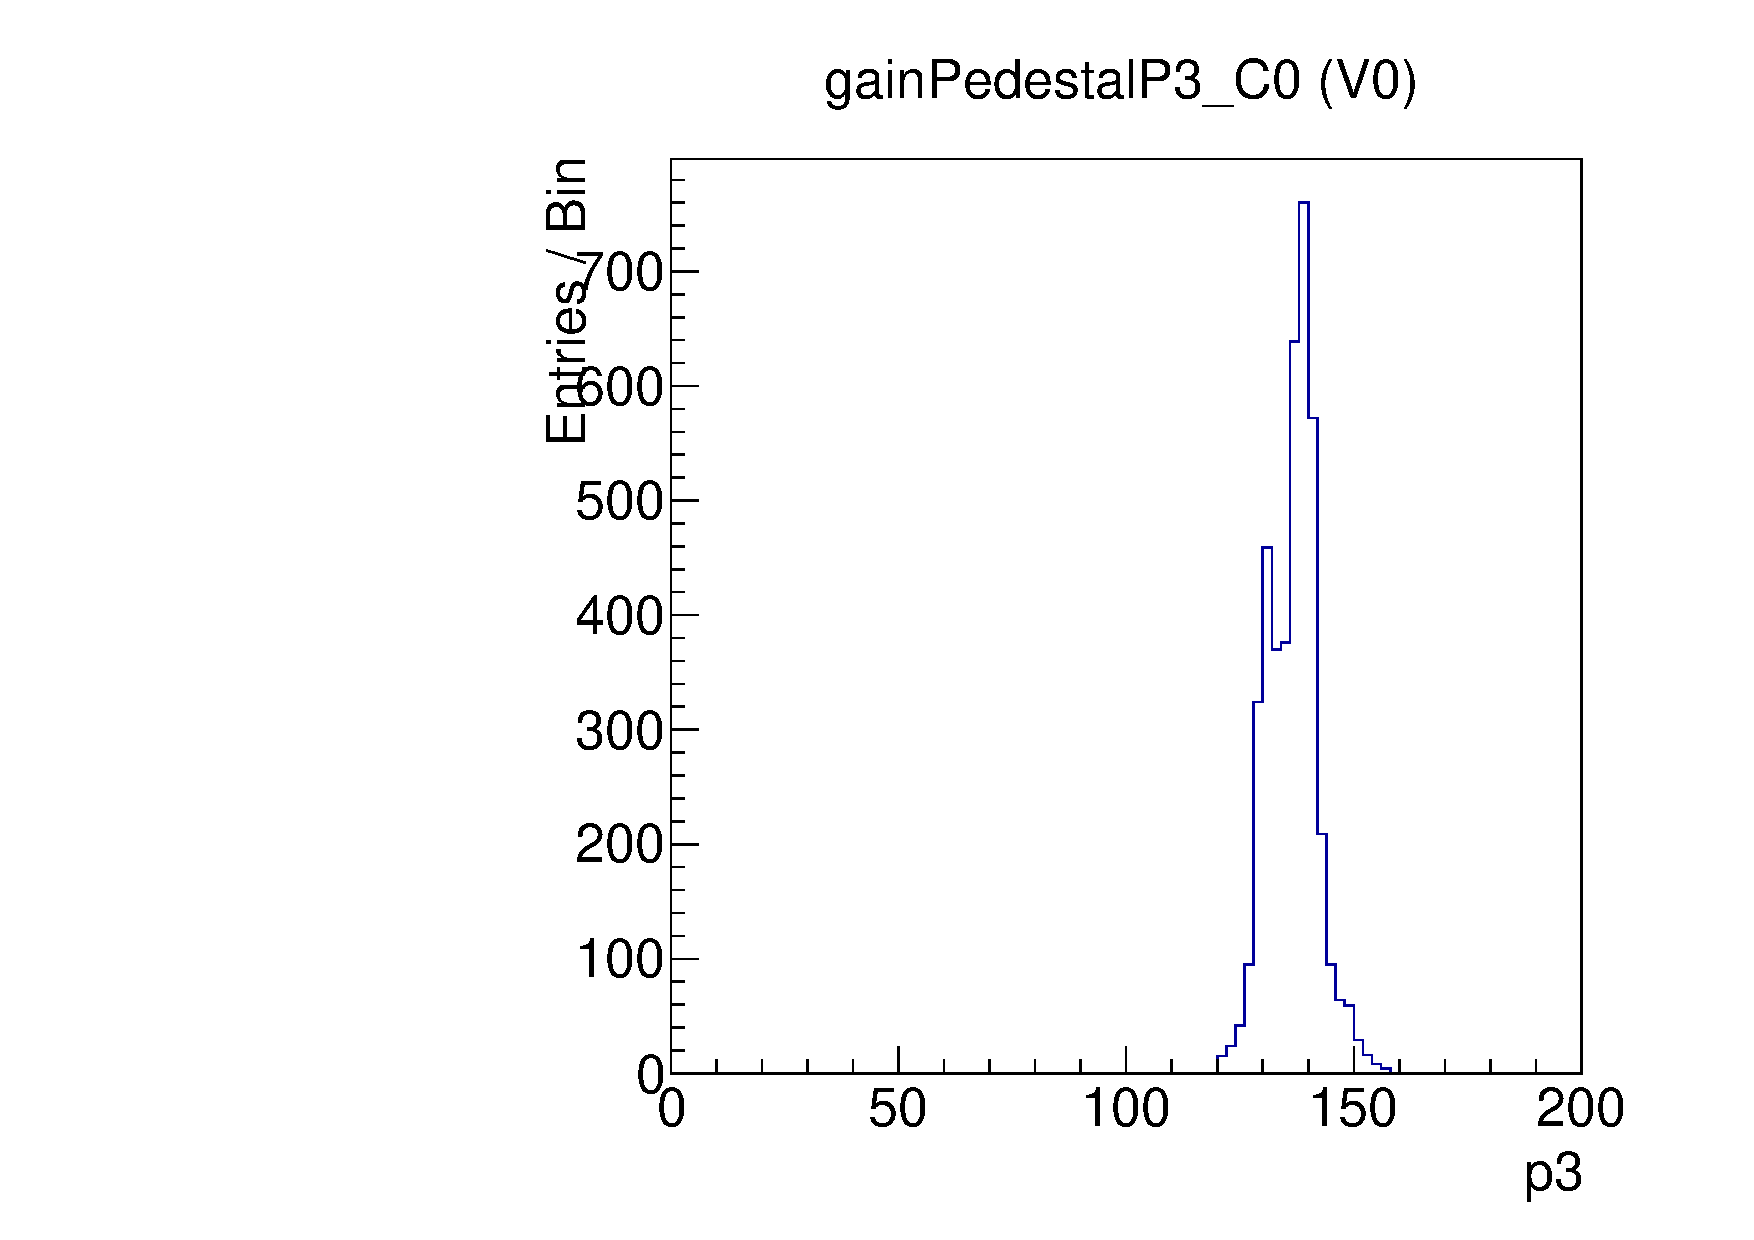
\includegraphics[width=1.0\textwidth]{figures/gainped_gainPedestalP3.pdf}
  \caption{}
  \label{fig:gainped_gainPedestalP3}
\end{minipage}
\hspace{0.3cm}
\begin{minipage}{0.45\textwidth}
  \includegraphics[width=1.0\textwidth]{figures/gainped_P3_relErr.pdf}
  \caption{}
  \label{fig:gainped_P3_relErr}
\end{minipage}
\end{figure}

\begin{figure}[!Hp]
\centering
\begin{minipage}{0.45\textwidth}
  \includegraphics[width=1.0\textwidth]{figures/gainped_gainPedestalNonLinearity.pdf}
  \caption{}
  \label{fig:gainped_gainPedestalNonLinearity}
\end{minipage}
\end{figure}


% ----------------------------------------------------------------------

\newpage

\subsection{\scurves Test}
\label{ss:scurves}

\subsubsection{Purpose}

The \scurves test as configured for FPix module testing has two primary purposes.
First, it evaluates the efficacy of the \trimming test.
Secondly, it measures the noise present in each pixel and can potentially flag abnormally noisy pixels.
Both of these goals are achieved by fitting the curve of efficiency vs. \vcal for each pixel.
The test gets its name from the shape of the error function used to fit the measured curve.

\subsubsection{Methodology}

An \scurves test is a generic type of test that measures a pixel's efficiency as a function of a chosen \dac.
Assuming the pixel will not respond at low values of the \dac in question and will be fully efficient at some higher value of the \dac,
the efficiency curve should have a region of zero efficiency, 
a transition region with increasing efficiency, and a plateau region with 100\% efficiency.
The shape of this curve mildly resembles the letter ``S''.
If no noise is present in the system the turn-on curve will be a simple step function, 
with the horizontal floor and plateau connected by a vertical line.
However, noise will reduce the slope of the line connecting the floor and plateau.
Using this fact, an estimate of the noise in the system can be extracted from the width of the turn-on curve.

For each pixel, the s-curve is fit with an error function, which is the cumulative distribution function for a Gaussian curve.
From this curve, three parameters are extracted.
The turn-on threshold, defined as the \dac value at which 50\% efficiency is reached, is denoted by the shorthand ``thr''.
The width of the turn-on curve, defined as the width parameter of the fitted error function, is denoted by the shorthand ``sig''.
Finally, the turn-off threshold, 
defined as the point above the turn-on threshold at which efficiency drops back below 50\%, is denoted by the shorthand ``thn''.

For the \scurves test as configured for FPix module testing, 
an \scurves test is performed over \vcal, in a \vcal range window around the target threshold for the \trimming test.
This is because, post-trimming, the expected region of the turn-on of the s-curve is known.
The number of triggers is configurable, but in order to extract accurate width values, 
a large number of triggers (default is 200) should be used.

\subsubsection{Output}

Figures~\ref{fig:scurves_thr_scurveVcal_Vcal}-\ref{fig:scurves_dist_thn_scurveVcal_Vcal} 
show the output of the \scurves test as used in the \fulltest for FPix module qualification.
\roc maps and 1D distributions of the three parameters measured by the test are saved in the output file: 
the turn-on ``thr'' (Figures~\ref{fig:scurves_thr_scurveVcal_Vcal},~\ref{fig:scurves_dist_thr_scurveVcal_Vcal}),
the width ``sig'' (Figures~\ref{fig:scurves_sig_scurveVcal_Vcal},~\ref{fig:scurves_dist_sig_scurveVcal_Vcal}),
and the turn-off ``thn'' (Figures~\ref{fig:scurves_thn_scurveVcal_Vcal},~\ref{fig:scurves_dist_thn_scurveVcal_Vcal}).
For s-curves with respect to \vcal, no turn-off is expected (it's mainly useful for \vthrcomp s-curves).
When no turn-off is observed, the test returns the maximum value of the \dac in question that is tested.

\begin{figure}[!htp]
\centering
\begin{minipage}{0.45\textwidth}
  \includegraphics[width=1.0\textwidth]{figures/scurves_thr_scurveVcal_Vcal.pdf}
  \caption{\roc map of the \vcal s-curve turn-on thresholds.
  Values should be near the trim target (default 35).}
  \label{fig:scurves_thr_scurveVcal_Vcal}
\end{minipage}
\hspace{0.3cm}
\begin{minipage}{0.45\textwidth}
  \includegraphics[width=1.0\textwidth]{figures/scurves_dist_thr_scurveVcal_Vcal.pdf}
  \caption{1D distribution of Figure~\ref{fig:scurves_thr_scurveVcal_Vcal}.
  [original range 0-255]}
  \label{fig:scurves_dist_thr_scurveVcal_Vcal}
\end{minipage}
\end{figure}

\begin{figure}[!htp]
\centering
\begin{minipage}{0.45\textwidth}
  \includegraphics[width=1.0\textwidth]{figures/scurves_sig_scurveVcal_Vcal.pdf}
  \caption{\roc map of the \vcal s-curve turn-on widths.  
  This width is proportional to the noise in the system.}
  \label{fig:scurves_sig_scurveVcal_Vcal}
\end{minipage}
\hspace{0.3cm}
\begin{minipage}{0.45\textwidth}
  \includegraphics[width=1.0\textwidth]{figures/scurves_dist_sig_scurveVcal_Vcal.pdf}
  \caption{1D distribution of Figure~\ref{fig:scurves_sig_scurveVcal_Vcal}.}
  \label{fig:scurves_dist_sig_scurveVcal_Vcal}
\end{minipage}
\end{figure}

\begin{figure}[!htp]
\centering
\begin{minipage}{0.45\textwidth}
  \includegraphics[width=1.0\textwidth]{figures/scurves_thn_scurveVcal_Vcal.pdf}
  \caption{\roc map of the \vcal s-curve turn-off thresholds.  
  For s-curves with respect to \vcal, no turn off is expected.
  Therefore this plot should be uniformly distributed at the maximum value of \vcal considered by the test.}
  \label{fig:scurves_thn_scurveVcal_Vcal}
\end{minipage}
\hspace{0.3cm}
\begin{minipage}{0.45\textwidth}
  \includegraphics[width=1.0\textwidth]{figures/scurves_dist_thn_scurveVcal_Vcal.pdf}
  \caption{1D distribution of Figure~\ref{fig:scurves_thn_scurveVcal_Vcal}.}
  \label{fig:scurves_dist_thn_scurveVcal_Vcal}
\end{minipage}
\end{figure}




% ----------------------------------------------------------------------

\newpage

\subsection{\bb Test}
\label{ss:bb}

\subsubsection{Purpose}

The \bb test is meant to flag any problems with the bump bonds that connect the sensor to the ROCs
and form the path for the charge generated in the silicon sensor to be recorded by the ROCs.
This test takes advantage of a parallel route designed for the calibration signal in the ROC.
This route can be seen at the top left of Figure~\ref{fig:puc}, 
connecting the source of the \vcal calibration pulse to the ``top metal pad'' 
by closing the switch labeled ``sensor calib'' instead of the standard ``calib'' switch.
The ``top metal pad'' is located near the edge of the \roc on the side facing the sensor.
The calibration pulse can pass via capacitive coupling from this pad, 
across the \roc-sensor air gap, and into the silicon sensor.
The calibration pulse then makes its way back into the \roc via the bump bond and can be read out as normal.
Using this signal path that contains the bump bond, 
the presence of the bump and the quality of the electrical connection it establishes between the sensor and the \roc can be tested.

Currently in pXar there are four variants of bump bonding tests, optimized to different module types.  
For FPix modules, the standard test is the {\tt BB3} test.
This document focuses on this specific \bb test version.

\subsubsection{Methodology}

The \bb test is essentially an \scurves test with respect to \vthrcomp, 
with the calibration signal routed through the sensor instead of directly to the readout electronics.
\vcal is configurable and by default is set to 250 (high range).
In any case, \vcal should be set quite high since a large signal loss is expected going through the air gap from \roc to sensor.
The number of triggers used is also configurable (default is 5).
From the \vthrcomp s-curve for each pixel, the turn on value is extracted, 
defined as the value of \vthrcomp for which the efficiency surpasses 50\%.
For pixels with good bump bonds, these thresholds should be distributed normally, i.e.~as a Gaussian curve.
The distribution of the \vthrcomp turn-on is fitted to a Gaussian, the mean and width of which are recorded.
In this fit, peaks near 0 or 255 are excluded, since these most likely come from dead pixels.
Since variations in the mean of this turn-on are observed in odd and even columns, 
this fitting is done separately for the odd/even columns in the \roc.
Pixels that turn on at much higher than average \vthrcomp values have higher than average signal loss.
Leveraging this fact, pixels with turn-on values more than $5\times\sigma$ above the mean are flagged as bad.

\subsubsection{Output}

Output from the \bb test is shown in Figures~\ref{fig:bb3_thr_calSMap_VthrComp}-\ref{fig:bb3_dist_rescaledThr}.
Figure~\ref{fig:bb3_thr_calSMap_VthrComp} shows a \roc map of the raw turn-on values extracted from the \vthrcomp s-curve for each pixel.
Figures~\ref{fig:bb3_dist_thr_calSMap_VthrComp_EvenCol} and \ref{fig:bb3_dist_thr_calSMap_VthrComp_OddCol} 
show the 1D distributions of the even and odd columns in Figure~\ref{fig:bb3_thr_calSMap_VthrComp}, 
along with their best-fit curves and arrows located $5\times\sigma$ above the mean of the curve.
The means of these distributions are noticeably different, which is why these two distributions are fit separately.
These distributions are then recombined, but since they have different means and widths,
it doesn't make sense to combine them directly.
Instead, each entry is scaled to represent the number of standard deviations it is away from the mean.
We refer to this scaled value as the fit ``residual''.
Figures~\ref{fig:bb3_rescaledThr} and \ref{fig:bb3_dist_rescaledThr} show a 2D \roc map and a 1D distribution of these fit residuals, respectively.
Any pixels above the black arrow in Figure~\ref{fig:bb3_dist_rescaledThr} are flagged as anomalous bumps.

\begin{figure}[!htp]
\centering
\begin{minipage}{0.45\textwidth}
  \includegraphics[width=1.0\textwidth]{figures/bb3_thr_calSMap_VthrComp.pdf}
  \caption{\roc map of the raw \vthrcomp turn-on values when passing the calibration pulse through the sensor.}
  \label{fig:bb3_thr_calSMap_VthrComp}
\end{minipage}
\end{figure}

\begin{figure}[!htp]
\centering
\begin{minipage}{0.45\textwidth}
  \includegraphics[width=1.0\textwidth]{figures/bb3_dist_thr_calSMap_VthrComp_EvenCol.pdf}
  \caption{1D distribution of the even columns in Figure~\ref{fig:bb3_thr_calSMap_VthrComp}.
  The red curve is a Gaussian fit to the data.
  The black arrow corresponds to 5$\sigma$ above the fitted peak.
  [original range 0-255]}
  \label{fig:bb3_dist_thr_calSMap_VthrComp_EvenCol}
\end{minipage}
\hspace{0.3cm}
\begin{minipage}{0.45\textwidth}
  \includegraphics[width=1.0\textwidth]{figures/bb3_dist_thr_calSMap_VthrComp_OddCol.pdf}
  \caption{1D distribution of the odd columns in Figure~\ref{fig:bb3_thr_calSMap_VthrComp}.
  The red curve is a Gaussian fit to the data.
  The black arrow corresponds to 5$\sigma$ above the fitted peak.
  [original range 0-255]}
  \label{fig:bb3_dist_thr_calSMap_VthrComp_OddCol}
\end{minipage}
\end{figure}

\begin{figure}[!htp]
\centering
\begin{minipage}{0.45\textwidth}
  \includegraphics[width=1.0\textwidth]{figures/bb3_rescaledThr.pdf}
  \caption{\roc map of the residuals of the \vthrcomp turn-on values, 
  calculated separately for even and odd columns.}
  \label{fig:bb3_rescaledThr}
\end{minipage}
\hspace{0.3cm}
\begin{minipage}{0.45\textwidth}
  \includegraphics[width=1.0\textwidth]{figures/bb3_dist_rescaledThr.pdf}
  \caption{1D distribution of \roc map in Figure~\ref{fig:bb3_rescaledThr}.
  Pixels with turn-on values more than 5$\sigma$ above the \roc mean 
  (marked by the black arrow) are flagged as faulty.
  The first (last) bin of the plot contains the underflow (overflow) entries.}
  \label{fig:bb3_dist_rescaledThr}
\end{minipage}
\end{figure}



% ----------------------------------------------------------------------

\newpage

\subsection{\iv Test}
\label{ss:iv}

\subsubsection{Purpose}

The \iv test is unique in that it doesn't directly utilize the read-out functionality of the \roc.
In fact, this test can be performed on a sensor before it's even bump-bonded onto a set of \rocs.
In principle, the silicon sensor acts like a diode, 
allowing current to flow in the ``forward'' direction but not in the ``reverse'' direction.
A potential difference is created across the sensor, in the plane transverse to the sensor face,
by applying a ``reverse bias'' voltage.
This potential difference is what draws the electrons created by a charged particle passing through the sensor 
towards the bump-bond to be collected.
For a given sensor, the reverse bias has an operating range.
If the bias is too small, the sensor will not be depleted of free electrons and will not operate properly.
If the bias is too large, the sensor will break down and start acting like a resistor instead of a diode.
The \iv test is meant to determine the operating range of the sensor, 
bounded by the depletion voltage (lower limit) and the breakdown voltage (upper limit).

\subsubsection{Methodology}

This test is exceedingly simple, it merely performs a scan over a range of bias voltages
and records the current draw of the system at each point.
During the test, control is taken over the HV supply in order to effect a voltage sweep.
The user can configure the range of voltages to scan (default is 0V-600V),
the step size between measurements (default 10V), 
and the amount of time between measurements to allow the system to react to the voltage change (default is 1s).
To protect the module from damage due to excessively high voltages, a compliance current is set (default is 100 $\mu$A).
If the current reaches this compliance level, the scan is aborted and the voltage turned off.
The single output from this test is a plot of the current draw as a function of the bias voltage
as shown in Figure~\ref{fig:iv_IVcurve}.
The module in question has an operating plateau from roughly -100V to -200V.

\subsubsection{Output}

\begin{figure}[!htp]
\centering
\begin{minipage}{0.45\textwidth}
  \includegraphics[width=1.0\textwidth]{figures/iv_IVcurve.pdf}
  \caption{Current draw in the module as a function of (reverse) bias voltage.
The module shown is fully depleted by -100V and shows a breakdown voltage near -200V.}
  \label{fig:iv_IVcurve}
\end{minipage}
\end{figure}


% ----------------------------------------------------------------------                                                                          

\newpage

\subsection{\fulltest}
\label{ss:fulltest}

The suite of tests that is run to qualify forward pixel modules is called the
\fulltest. It is a sequential test suite composed of the following tests
that are described in more detail in the previous sections.
\begin{itemize}
  \item \pretest: configures the basic \dacs to ensure that the \roc is in a functioning state.
  \item \alivetest: checks that all pixels respond to an input signal,
  have the correct addresses associated with them, and can be masked. 
  \item \trimming: sets all pixels to turn on with the same input signal strength
  \item \phopt: optimizes the dynamic range of the output pulse heights as calculated by the ADC serializer
  \item \gainped: measures and stores the gain and pedestal of each pixel and checks the linearity of the ADC response
  \item \scurves: measures pixel threshold and noise, validates the trimming
  \item \bb: flags potential issues in bump bond quality
\end{itemize}
In addition to the \fulltest, each module undergoes an \iv test that measures leakage current as a function of the reverse bias voltage.
For technical reasons described in Section~\ref{s:testing}, this test is performed separately from the \fulltest.


% ----------------------------------------------------------------------

%\newpage
% ======================================================================
\section{Module Testing at FNAL}
\label{s:testing}
% ======================================================================

% ----------------------------------------------------------------------

\subsection{Experimental setup}
\label{ss:setup}

All module testing at FNAL takes place at the Silicon Detector laboratory (SiDet).
There are two identical FPix module testing stands at SiDet situated next to each other.
Figure~\ref{fig:setup} shows one such test stand.
Up to four modules can be tested in parallel.
The modules are connected via copper cables to adapter cards with SMK connectors.
The adapter cards convert the data into SCSI format.
A SCSI cable from each adapter card transfers the data to a digital test board (DTB), which is in turn connected via USB to a PC.
There are two power supplies in the setup.
The first provides the bias voltage to the sensors under test by way of a four-way splitter (top box in Figure~\ref{fig:setup}).
The other provides power to the cooling system of the coldbox (bottom box in Figure~\ref{fig:setup}).
The water chiller, vacuum, and coldbox work together to control the temperature of the modules under test.
Each test stand also has a dry air ($\textrm{N}_2$) line that connects to the coldbox to help control the humidity inside it.

\begin{figure*}[hbtp]
\begin{center}
\includegraphics[width=\textwidth]{figures/fnal_test_stand.pdf}
\caption{An annotated photo of one of two identical module testing setups at SiDet.}
\label{fig:setup}
\end{center}
\end{figure*}

\subsection{Safety concerns}
\label{ss:safety}

There are several safety precautions that should be taken to minimize potential damage to the modules.
Generally speaking, there are three sources of potential damage: 
physical damage, electrostatic discharge (ESD), and damage due to condensation.
To avoid these hazards, the following guidelines should be followed whenever modules are involved.
\begin{itemize}
\item The module cover protects the HDI and sensitive wirebonds from mishandling.
Do not remove it under normal testing circumstances.
\item Likewise, the lid of the coldbox protects the modules from the afore-mentioned damages.  
Never open the cover while module testing is taking place.  
In fact, the handle of the coldbox lid will shock you if you touch it during testing, and it will hurt a lot.
Once module testing is complete, wait until the coldbox has reached room temperature before removing the modules.
\item Whenever handling a module, make sure you are grounded via the provided wrist straps and bracelets.
There are also ESD-safe mats on the surface of the test stand table and on the floor underneath the test stand.
\item When not being tested, modules should be placed in the pink ESD-safe sleeves and stored in one of the designated cabinets.
These cabinets are fed with dry air to maintain low humidity.
\end{itemize}

\subsection{Testing procedure}
\label{ss:procedure}

The standard test sequence for modules is the \fulltest, as outlined in Section~\ref{ss:fulltest}, following by an \iv curve.
Each module will be tested once near room temperature ($17^\circ\,$C) 
and once closer to the operating temperature of the FPix in CMS ($-20^\circ\,$C).
The first 100 production-level modules all will undergo X-ray testing in between the \fulltest at $17^\circ\,$C and the \fulltest at $-20^\circ\,$C.
After the first 100, only a subset of modules (roughly 10\%) will undergo X-ray testing.

The {\tt elComandante} software package is used to facilitate parallel module testing.
More information can be found here: 
\begin{center}
https://twiki.cern.ch/twiki/bin/viewauth/CMS/ElComandante
\end{center}
This package allows simultaneous control of all the dynamic elements of the test setup (four DTBs, HV supply, and coldbox).
Once modules are installed in the coldbox, 
the water chiller is turned on (default water temperature is 10 C) and the coldbox is cooled to the desired temperature.
Once the temperature has stabilized, 
the standard procedure is to run the \fulltest in parallel on four modules, followed by four individual \iv curves.
The \iv test doesn't directly use the DTB, it simply reads the current directly from the power supply.
Since the same HV supply is used for all modules under test, parallel \iv scans are not possible.
When all tests have finished, the coldbox automatically heats (if necessary) until room temperature is reached.
At this point the modules can be safely removed from the coldbox and placed in storage.

Specific instructions for the shifters who will be testing modules can be found here:
\begin{center}
https://twiki.cern.ch/twiki/bin/viewauth/CMS/FPIXUpgradeShifterInstructions.
\end{center}

% ======================================================================
\section{Test Result Databases}
\label{s:uploading}
% ======================================================================


% ----------------------------------------------------------------------

Once a module has been tested, the resulting information is uploaded onto two remote servers:
One for visualization and one for documentation.
The shifters will execute provided scripts that format the test results appropriately 
and upload them to both of these servers.
The visualization is achieved via the {\tt MoReWeb} software package which processes the test results
and creates a set of html pages to help nagivate through the results of a given module.
This server can be accessed here: 
\\
http://www.physics.purdue.edu/cmsfpix/MoReWeb/Results/Overview.html
\\
The documenting of test results and grading of modules is done by the Purdue FPix database, found here: 
\\
http://www.physics.purdue.edu/cmsfpix/Submission\_p/index.php
\\
This database tracks module components from their origins through their inclusion in FPix modules.
It also stores all the configuration files and output root files generated during module testing.  
It has the functionality to search through the entire set of constructed modules, filtering on grade, location, etc.



% ======================================================================
\section{Module Grading Scheme}
\label{s:grading}
% ======================================================================


% ----------------------------------------------------------------------

Each FPix phase 1 upgrade module is given a grade based on various aspects of the testing results.
The current grading scheme is preliminary and expected to evolve through the production process
to account for specific component failure modes seen during production.
\\\\
The current scheme is based on two categories (\iv performance and single pixel defects)
although it can be expanded to include X-ray results and many of the other \fulltest measurements.
\\\\
The \iv performance criteria are two-fold.  
First, the module is graded on the amount of leakage current at the expected operating bias (-150V).
Modules must have $\textrm{I}_{-150\textrm{V}} < 2 \mu \textrm{A}$ to receive an A
or $\textrm{I}_{-150\textrm{V}} < 10 \mu \textrm{A}$ to receive a B.
Modules with $\textrm{I}_{-150\textrm{V}} > 10 \mu \textrm{A}$ receive a C.
Secondly, the breakdown voltage for the module should be higher (more negative) than -150V.
This is determined by looking at the ratio $\textrm{I}_{-150\textrm{V}}/\textrm{I}_{100\textrm{V}}$.
If the module has not reached the breakdown voltage by -150V, this ratio should be small, 
otherwise it should be large.
Modules with $\textrm{I}_{-150\textrm{V}}/\textrm{I}_{100\textrm{V}} < 2$ receive an A for this criteria,
all other modules receive a C.
The overall \iv grade for the module is the worse of these two assigned grades (leakage current and breakdown voltage).
\\\\
Single pixel defects are identified using the results of the \alivetest and \bb tests.
A sum per \roc is calculated of all pixels flagged as faulty by either of these tests.
If this sum is less than 1\% of pixels in the \roc, the \roc receives an A grade.
Otherwise, if the sum is less than 4\% of pixels in the \roc, the \roc receives an B grade.
If not, the \roc receives a C grade.
The module grade for single pixel defects is assigned as the grade of the worst \roc.
\\\\
The final module grade is assigned as the worse of the \iv grade and the pixel defect grade.
In this way, each module is given either an A, B, or C grade that is recorded in the documentation server.


%\newpage
%\printglossaries

%\newpage
%\clearpage
%\phantomsection
%\addcontentsline{toc}{chapter}{References}
%\addcontentsline{toc}{section}{References}
%\begin{thebibliography}{99}
%  \input{usermanual/references.tex}
%\end{thebibliography}  


\end{document}
